% Compile:
%   pdflatex report.tex
%   pdflatex report.tex
% or:
%   latexmk -pdf report.tex

\documentclass[11pt]{article}

\usepackage[margin=1in]{geometry}
\usepackage[T1]{fontenc}
\usepackage{lmodern}
\usepackage{microtype}

\usepackage{graphicx}
\usepackage{booktabs}
\usepackage{tabularx}
\usepackage{float}
\usepackage{subcaption}
\usepackage{hyperref}

\hypersetup{
  colorlinks=true,
  linkcolor=blue,
  urlcolor=blue,
  citecolor=blue
}

\graphicspath{{outputs/}}

\title{Global Food Trade Network Analysis\\\large Networks and Complex Systems Course Report}
\author{Chaitanya Attanti \\ Avinash Reddy}
\date{21 April 2026}

\begin{document}
\maketitle

\begin{abstract}
We analyze the global food trade system as a directed, weighted network in which nodes are countries and edges represent bilateral export flows. The goal is to characterize concentration, identify critical corridors and countries, and assess robustness under random failures and targeted disruptions. Results indicate a hub-dominated, heavy-tailed structure: a small subset of countries and routes accounts for a large share of connectivity and trade value, producing efficiency in normal operation but fragility under targeted removal.
\end{abstract}

\section{Introduction: Global Food Trade as a Network}
\subsection{Project overview}
This report models global food trade as a directed weighted graph with $N=198$ countries (nodes) and $M=18{,}242$ directed trade routes (edges). Edge direction follows exporter $\rightarrow$ importer and edge weight captures trade value. The analysis aims to identify concentration, structural bottlenecks, and robustness properties relevant to systemic risk and food security.

\subsection{Dataset foundation}
\begin{itemize}
  \item \textbf{Input edge list:} a pre-built directed edge list (CSV) of country-to-country food flows.
  \item \textbf{Network construction:} directed graph where source$\rightarrow$receiver represents export flow.
  \item \textbf{Edge weights:} trade value used for weighted centralities and damage curves.
  \item \textbf{Geographic data:} country coordinates used for world map visualizations.
\end{itemize}

\begin{figure}[H]
  \centering
  \includegraphics[width=0.98\linewidth]{04_core_network.png}
  \caption{Global food trade network visualization (directed, weighted).}
  \label{fig:core-network}
\end{figure}

\begin{figure}[H]
  \centering
  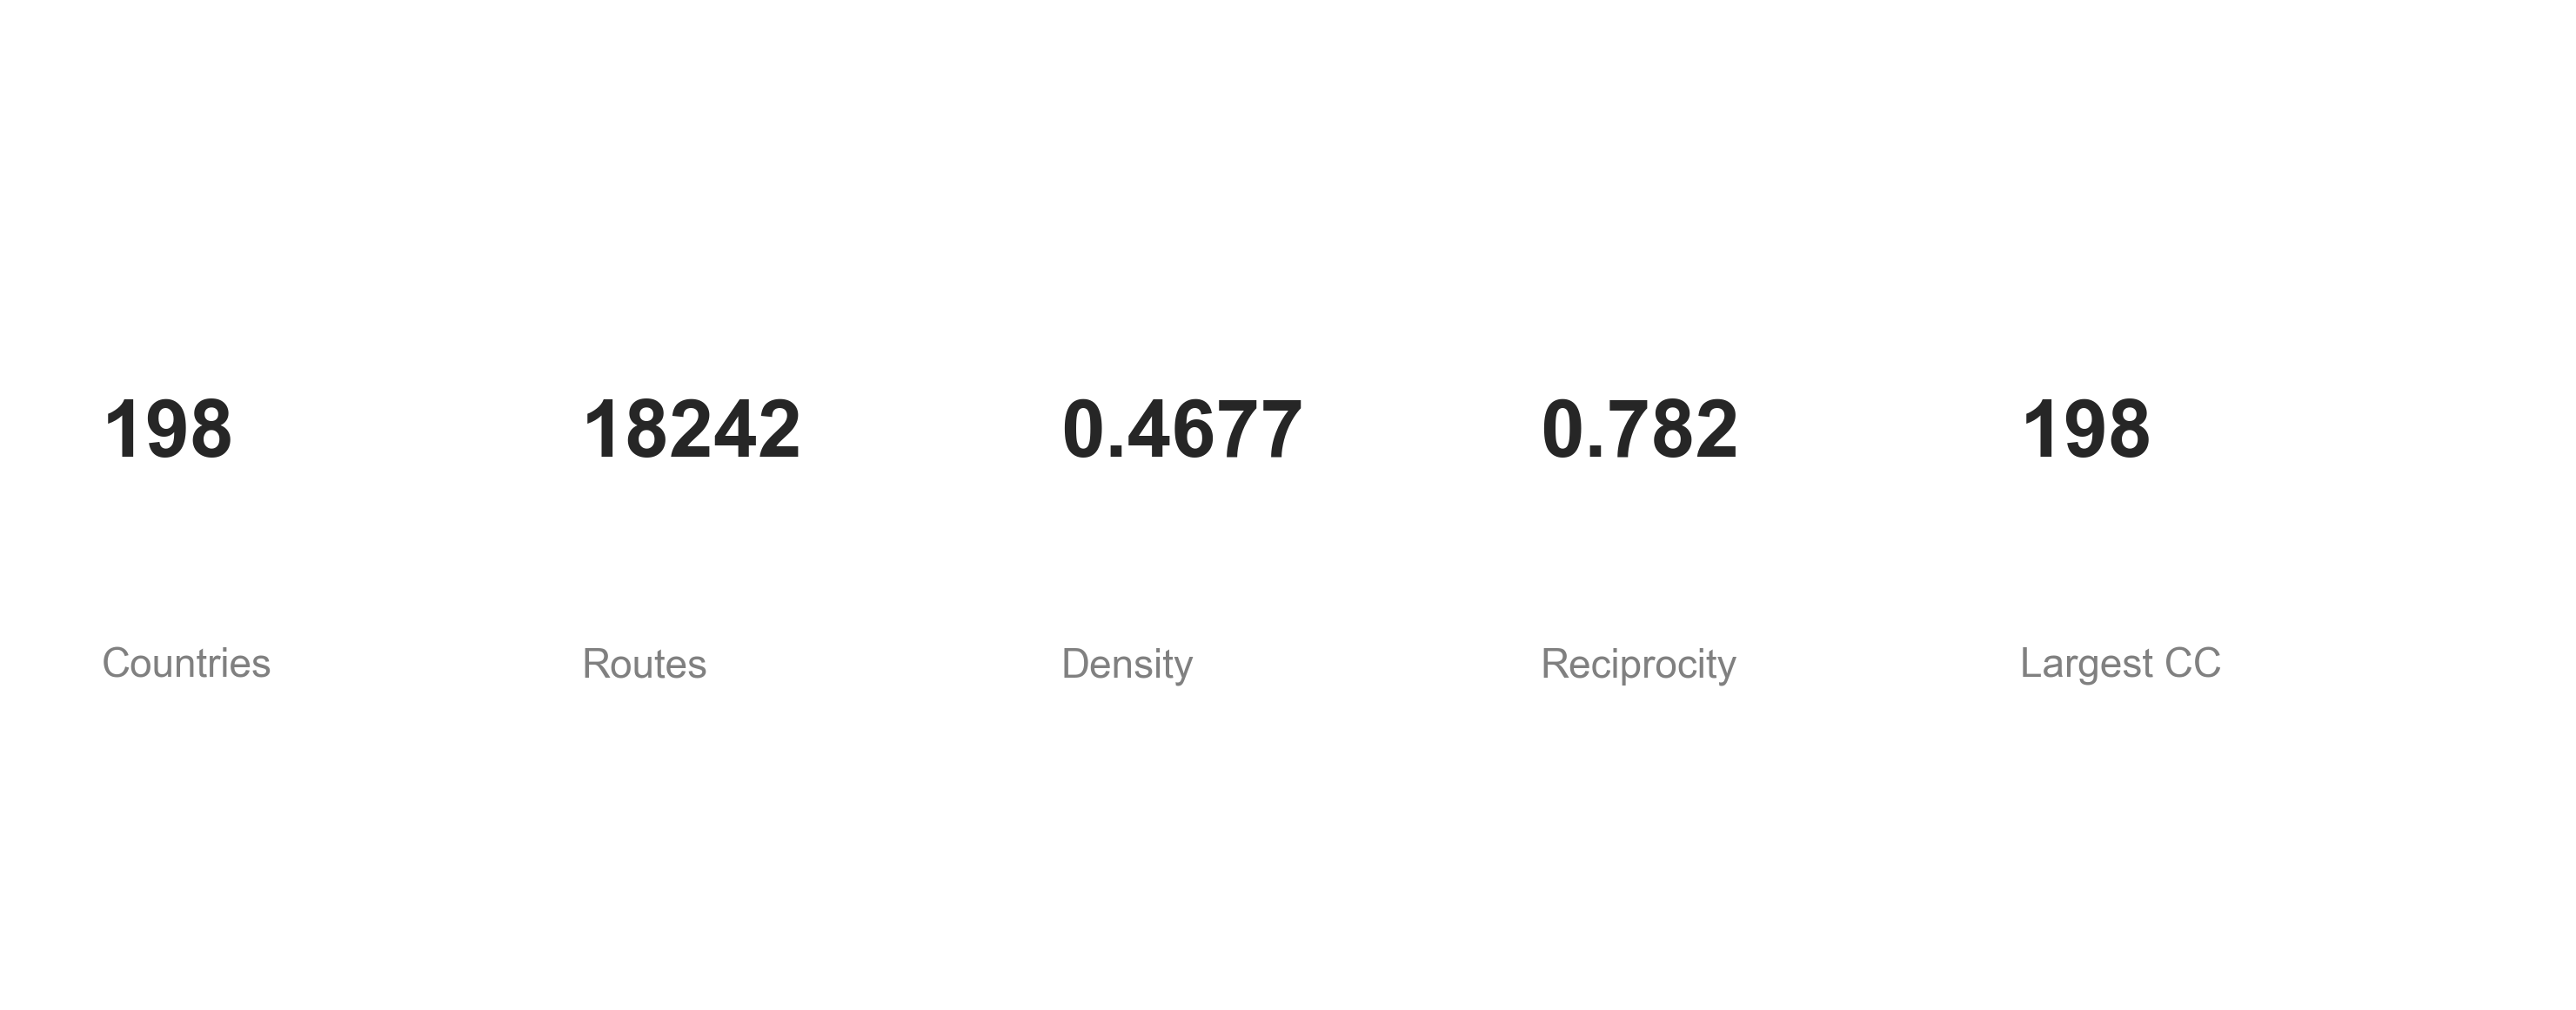
\includegraphics[width=0.98\linewidth]{31_intro_metrics.png}
  \caption{Key network statistics summary used throughout the analysis.}
  \label{fig:intro-metrics}
\end{figure}

\begin{figure}[H]
  \centering
  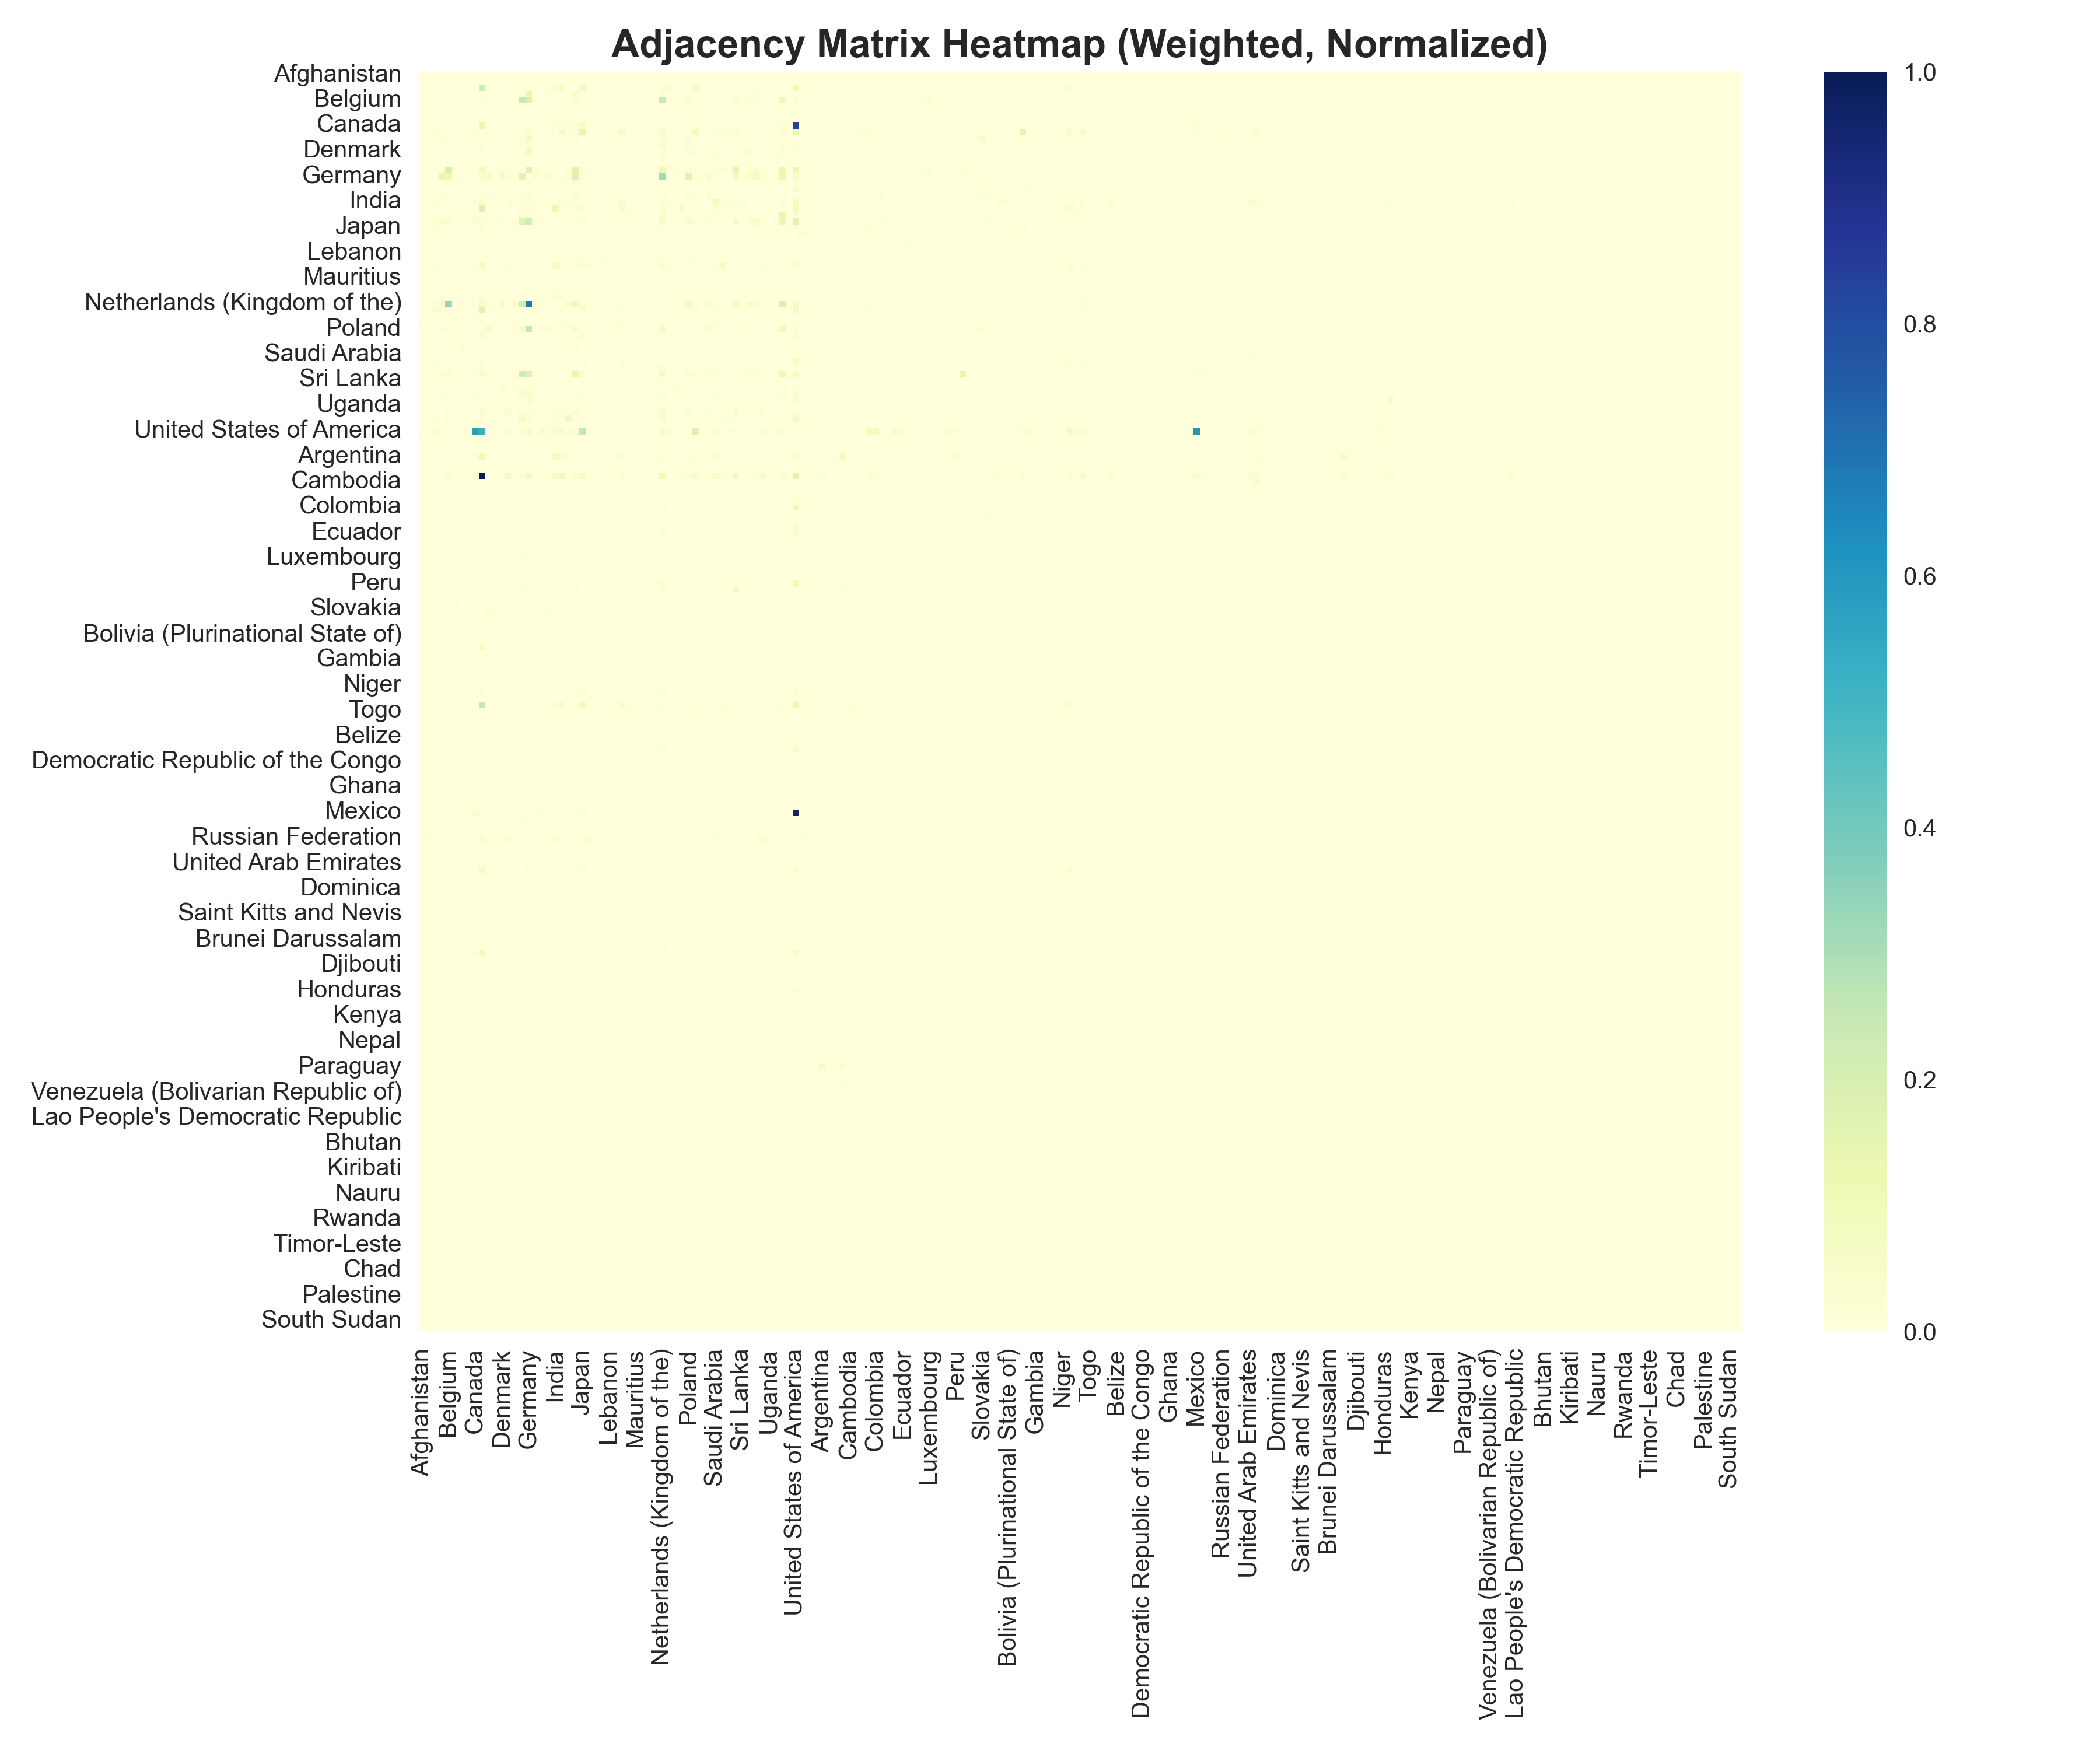
\includegraphics[width=0.98\linewidth]{21_adjacency_heatmap.png}
  \caption{Adjacency matrix heatmap (normalized weights). Strong flows concentrate in limited regions of the country-by-country matrix.}
  \label{fig:adjacency-heatmap}
\end{figure}

\begin{figure}[H]
  \centering
  \begin{subfigure}[t]{0.49\linewidth}
    \centering
    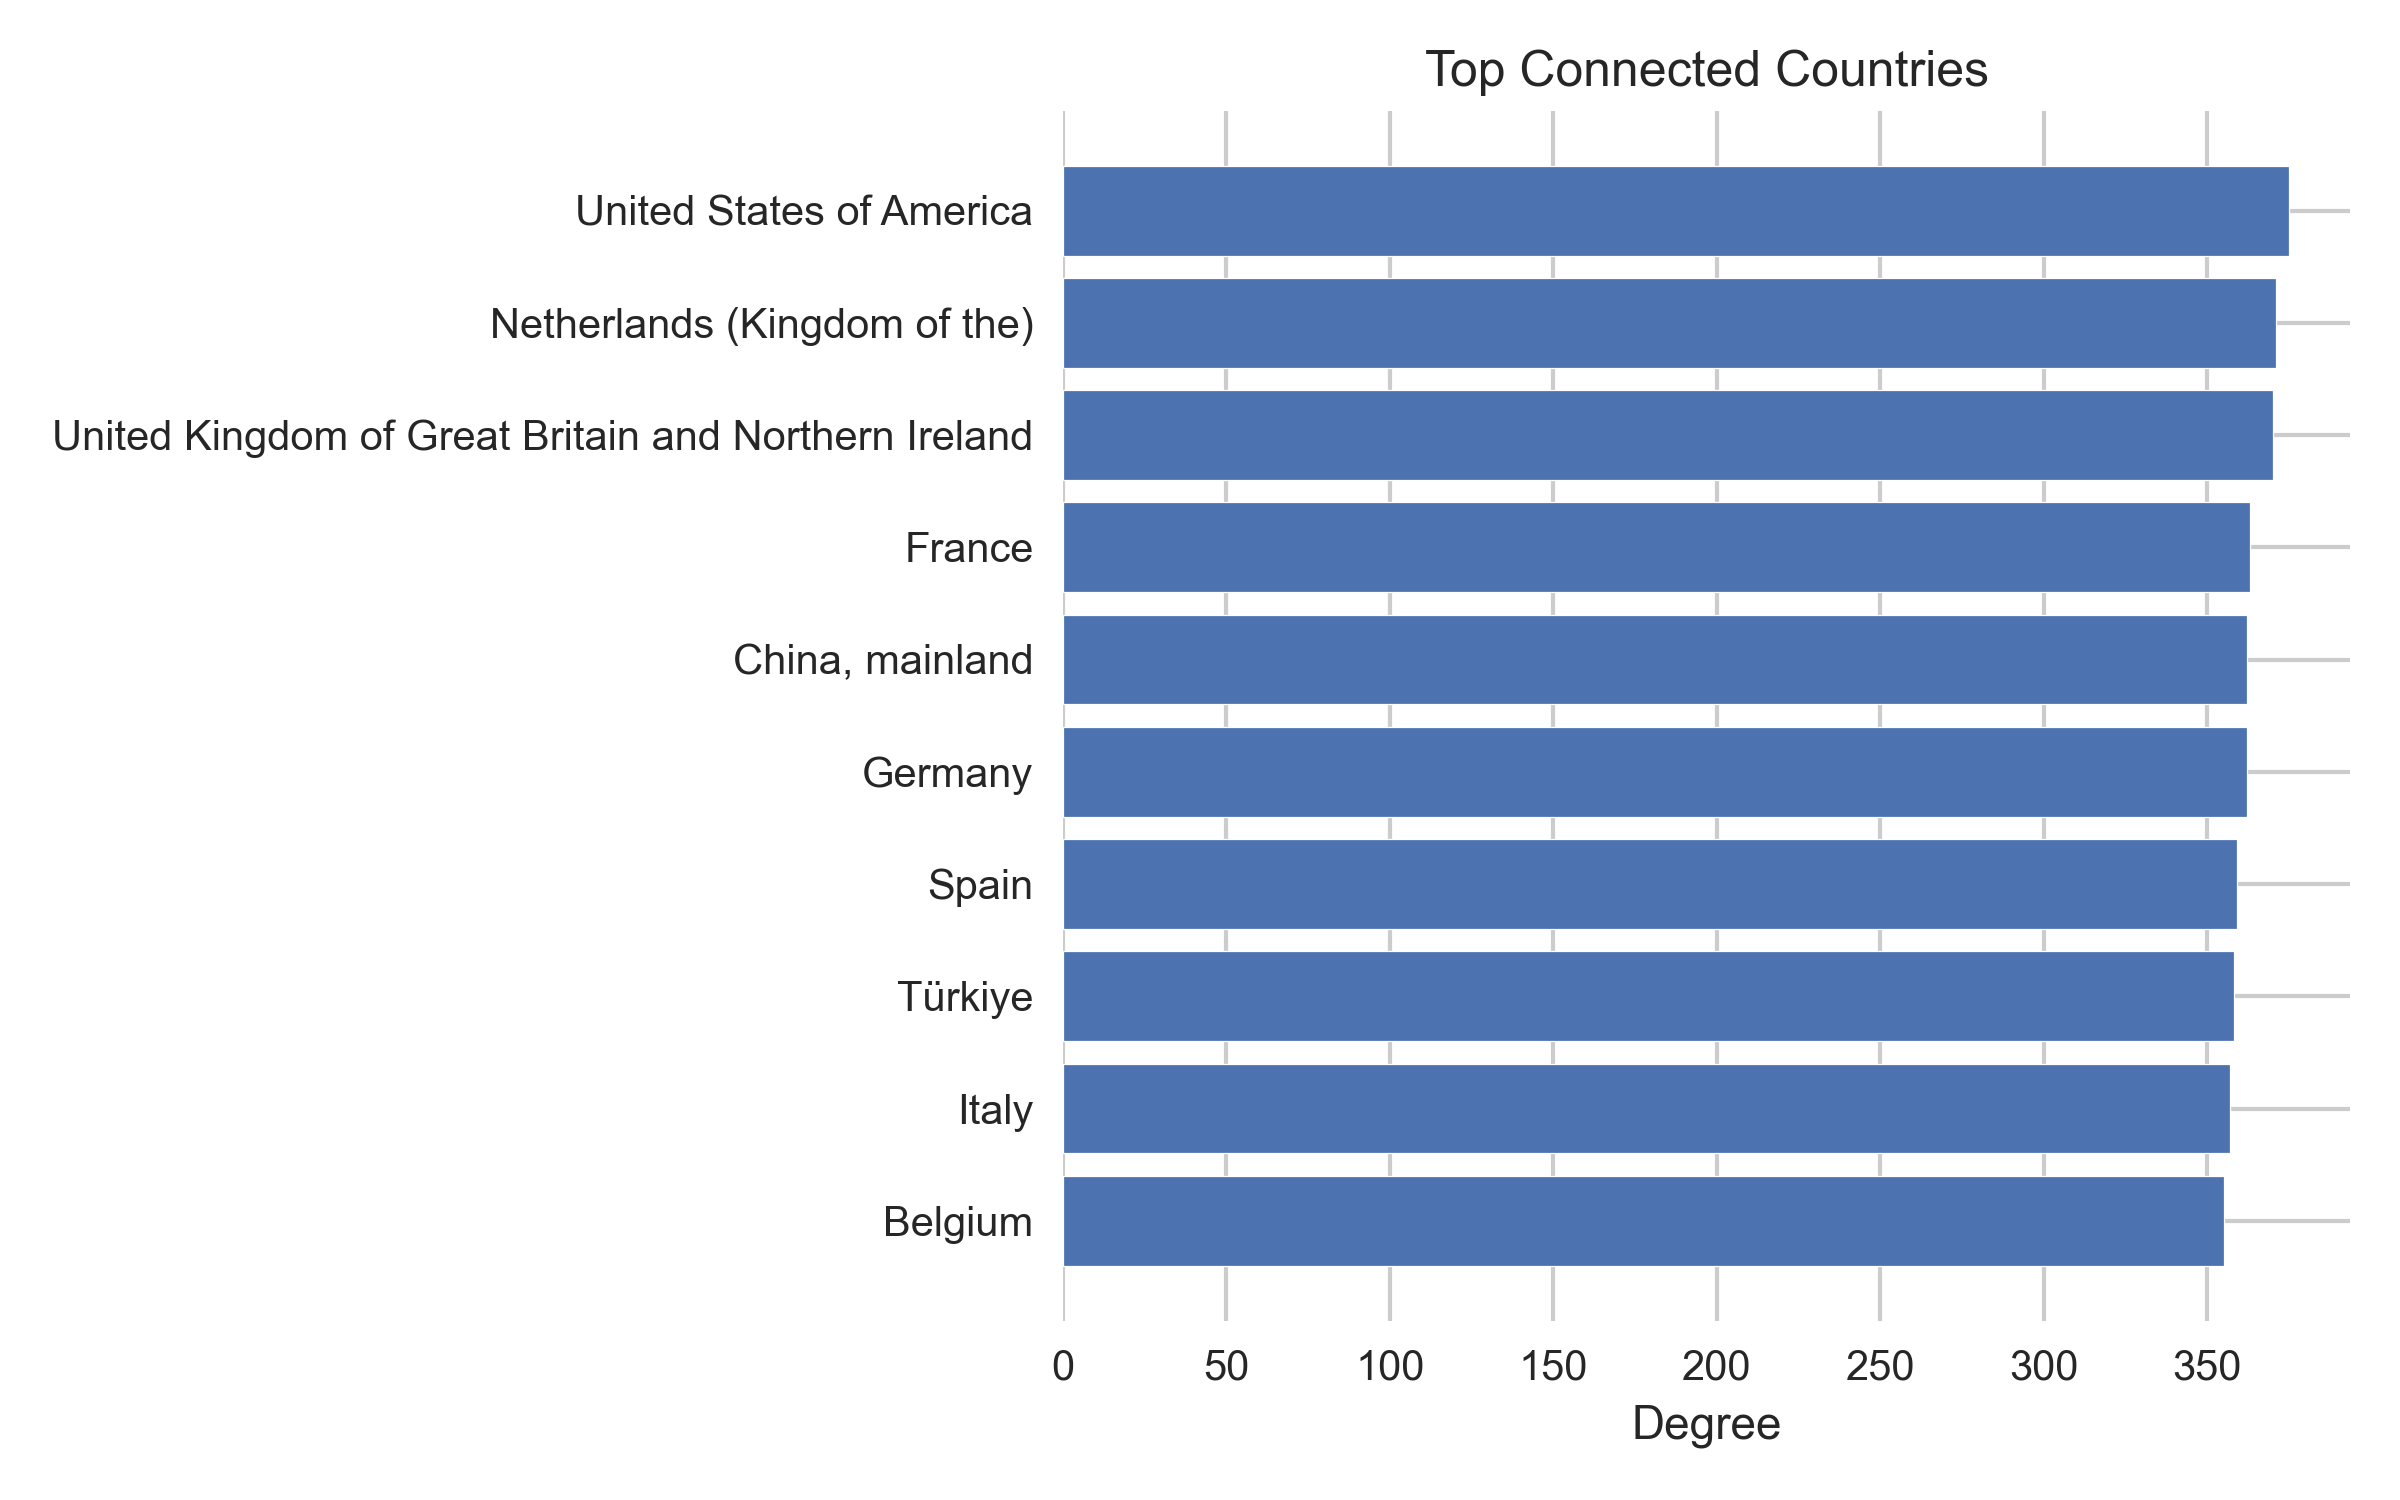
\includegraphics[width=\linewidth]{33_intro_top_connected.png}
    \caption{Most connected countries (highest partner counts).}
  \end{subfigure}
  \hfill
  \begin{subfigure}[t]{0.49\linewidth}
    \centering
    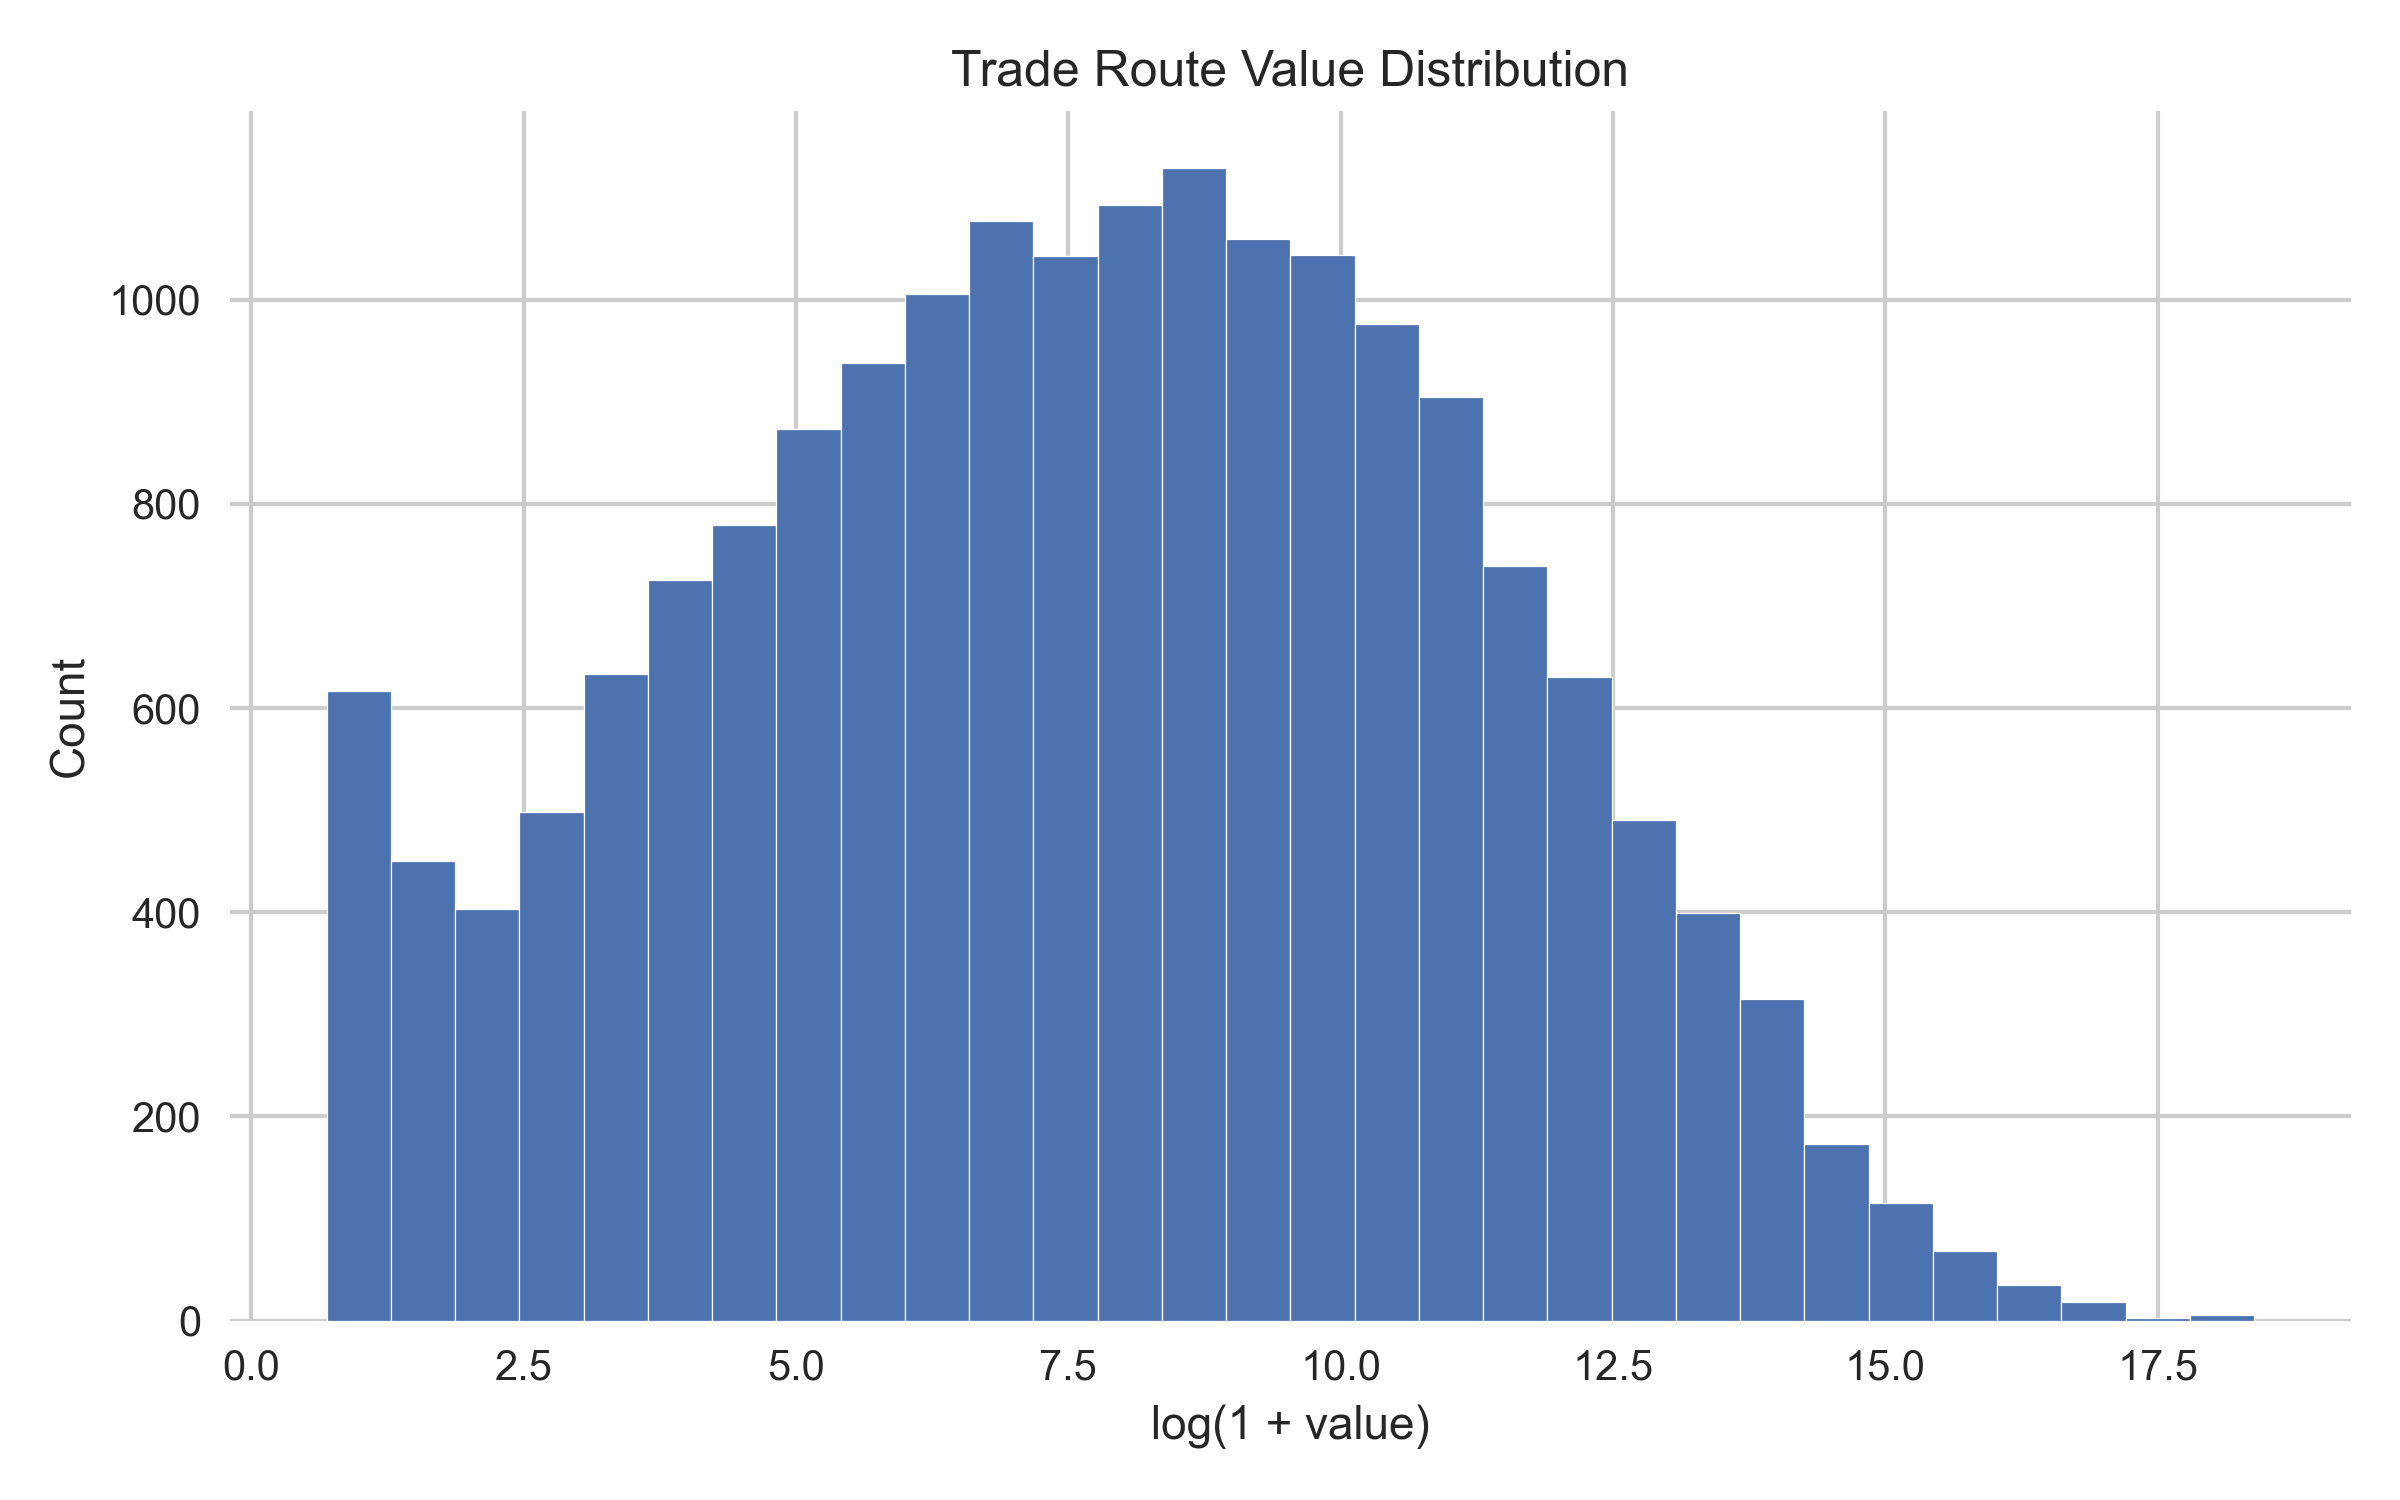
\includegraphics[width=\linewidth]{34_intro_trade_hist.png}
    \caption{Trade-value distribution across routes.}
  \end{subfigure}
  \caption{Introductory views of connectivity and edge-weight distributions.}
  \label{fig:intro-panels}
\end{figure}

\section{Concentration: Few Nodes and Few Links Dominate}
This section evaluates concentration risk: whether connectivity and trade value are broadly distributed or dominated by a small subset of countries and corridors.

\subsection{Heavy-tailed structure}
\begin{figure}[H]
  \centering
  \begin{subfigure}[t]{0.49\linewidth}
    \centering
    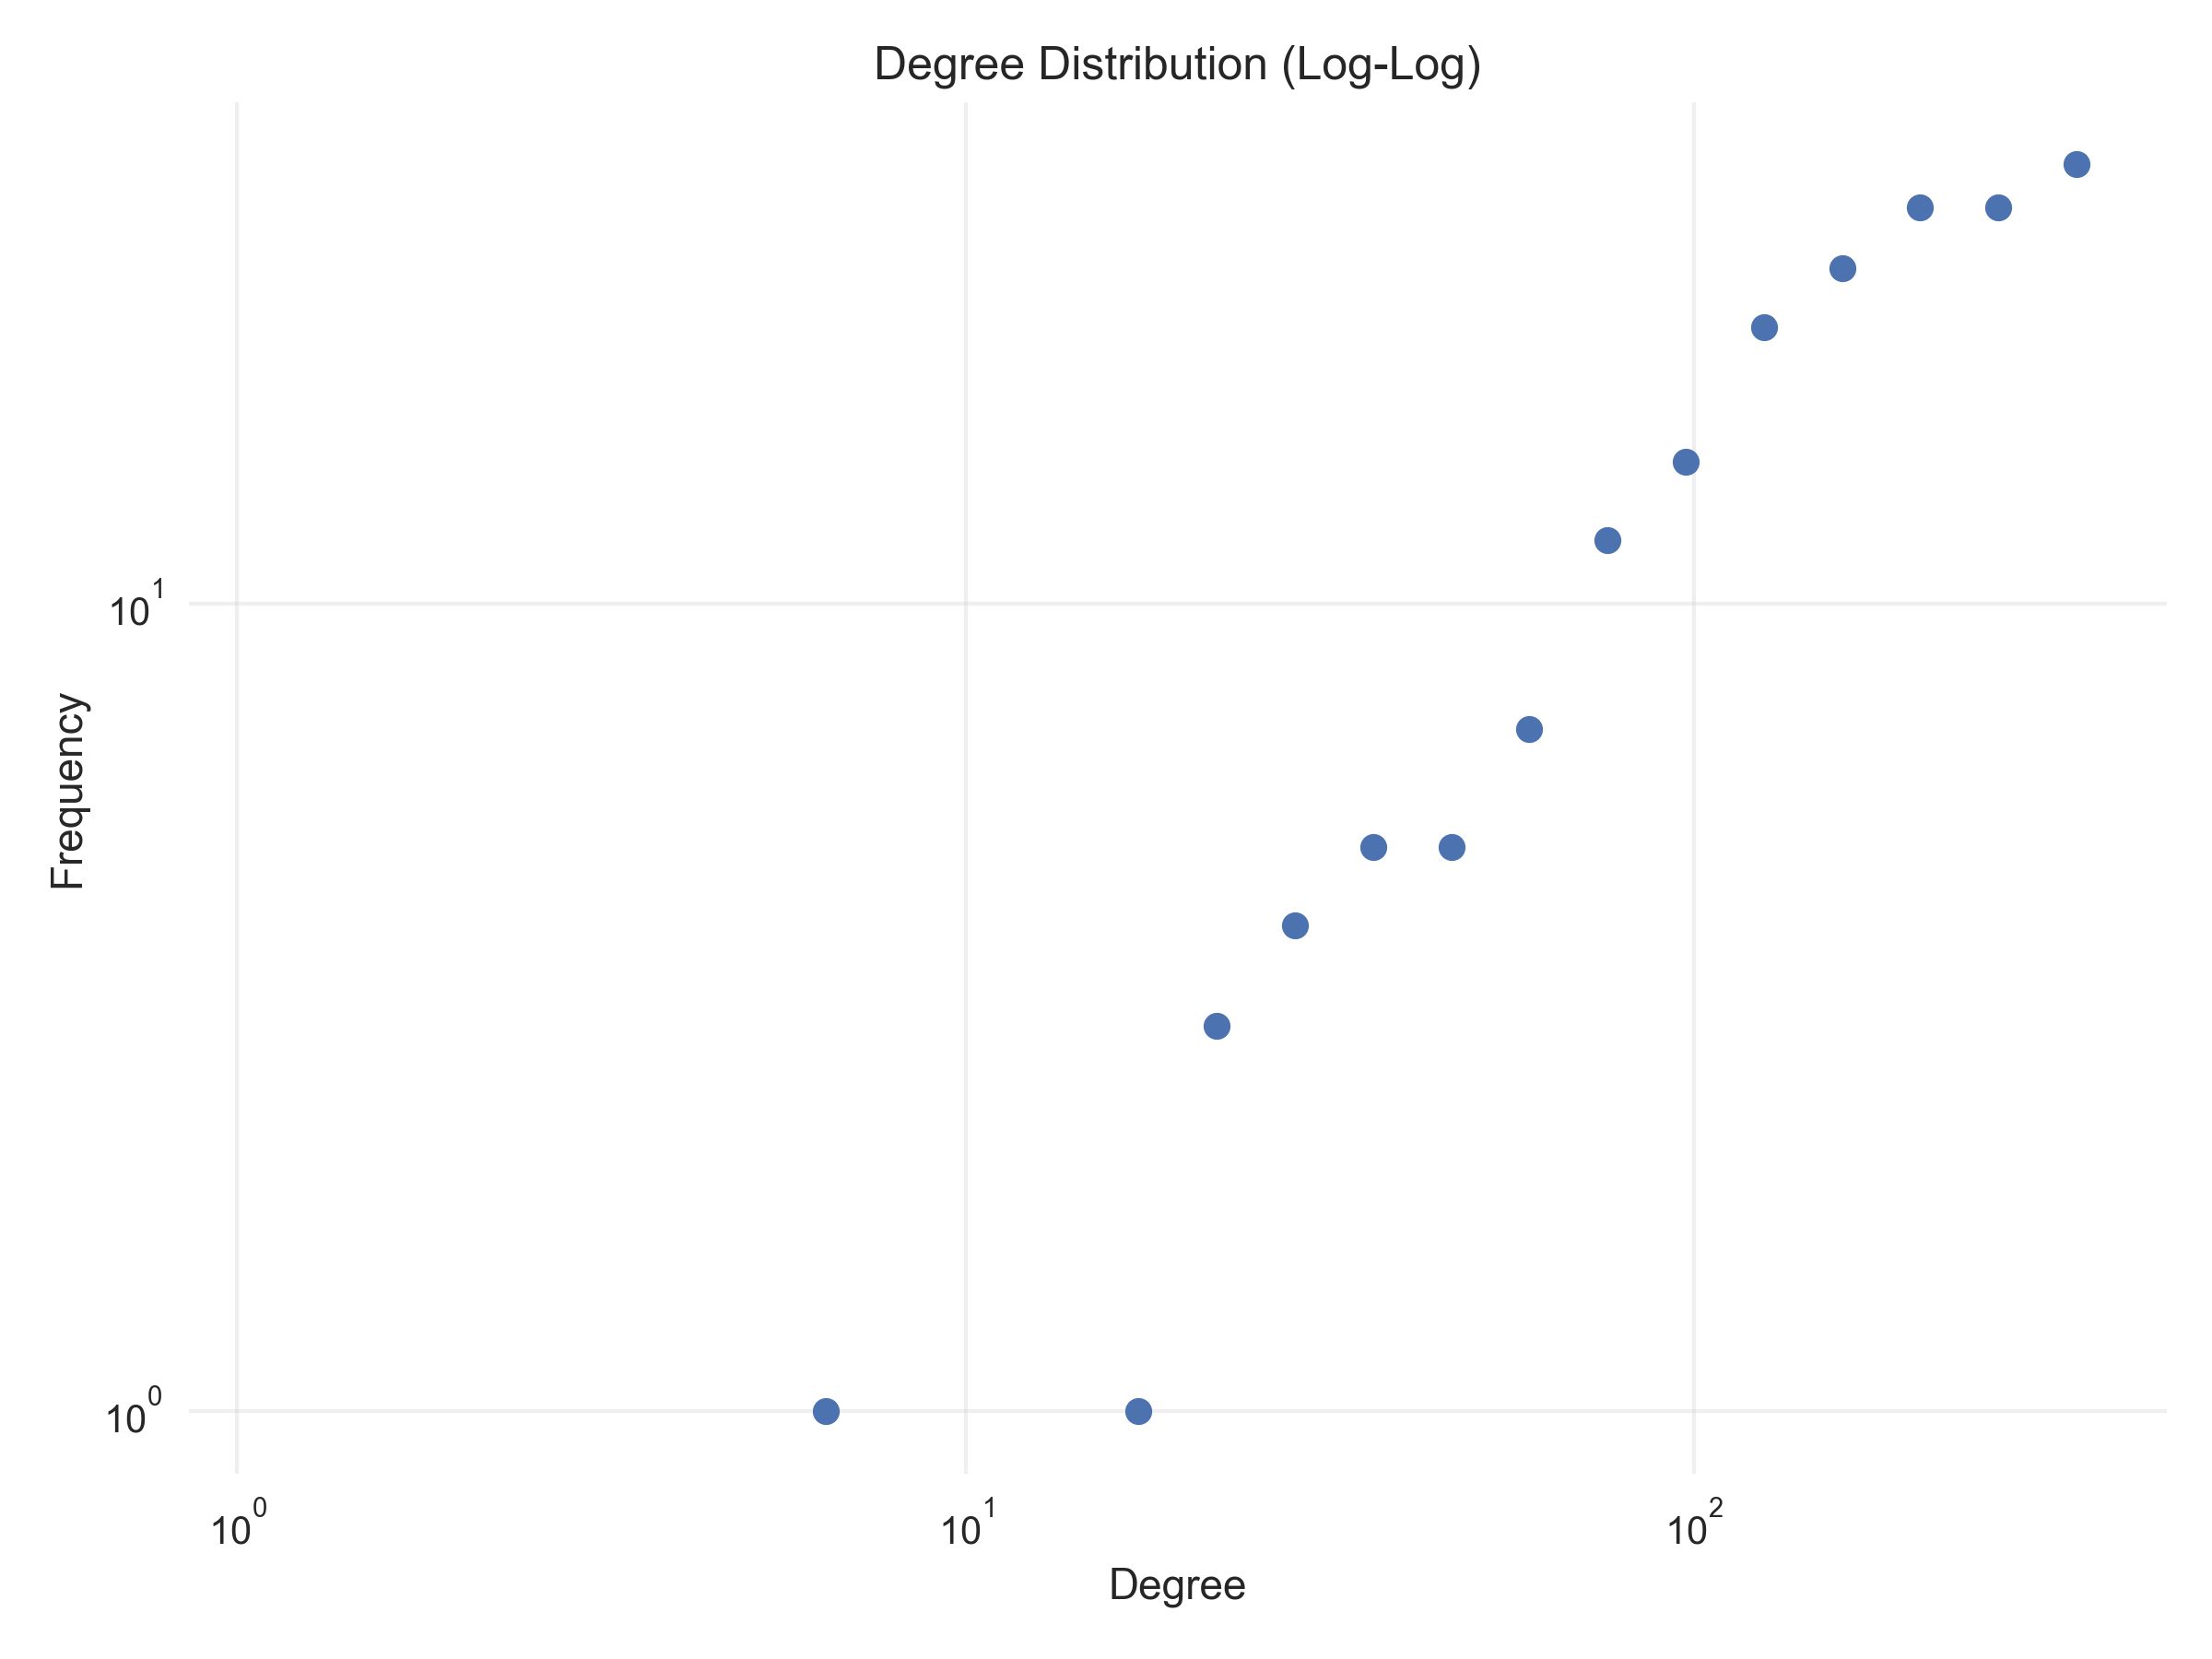
\includegraphics[width=\linewidth]{25_degree_hist_loglog.png}
    \caption{Degree distribution (log--log).}
  \end{subfigure}
  \hfill
  \begin{subfigure}[t]{0.49\linewidth}
    \centering
    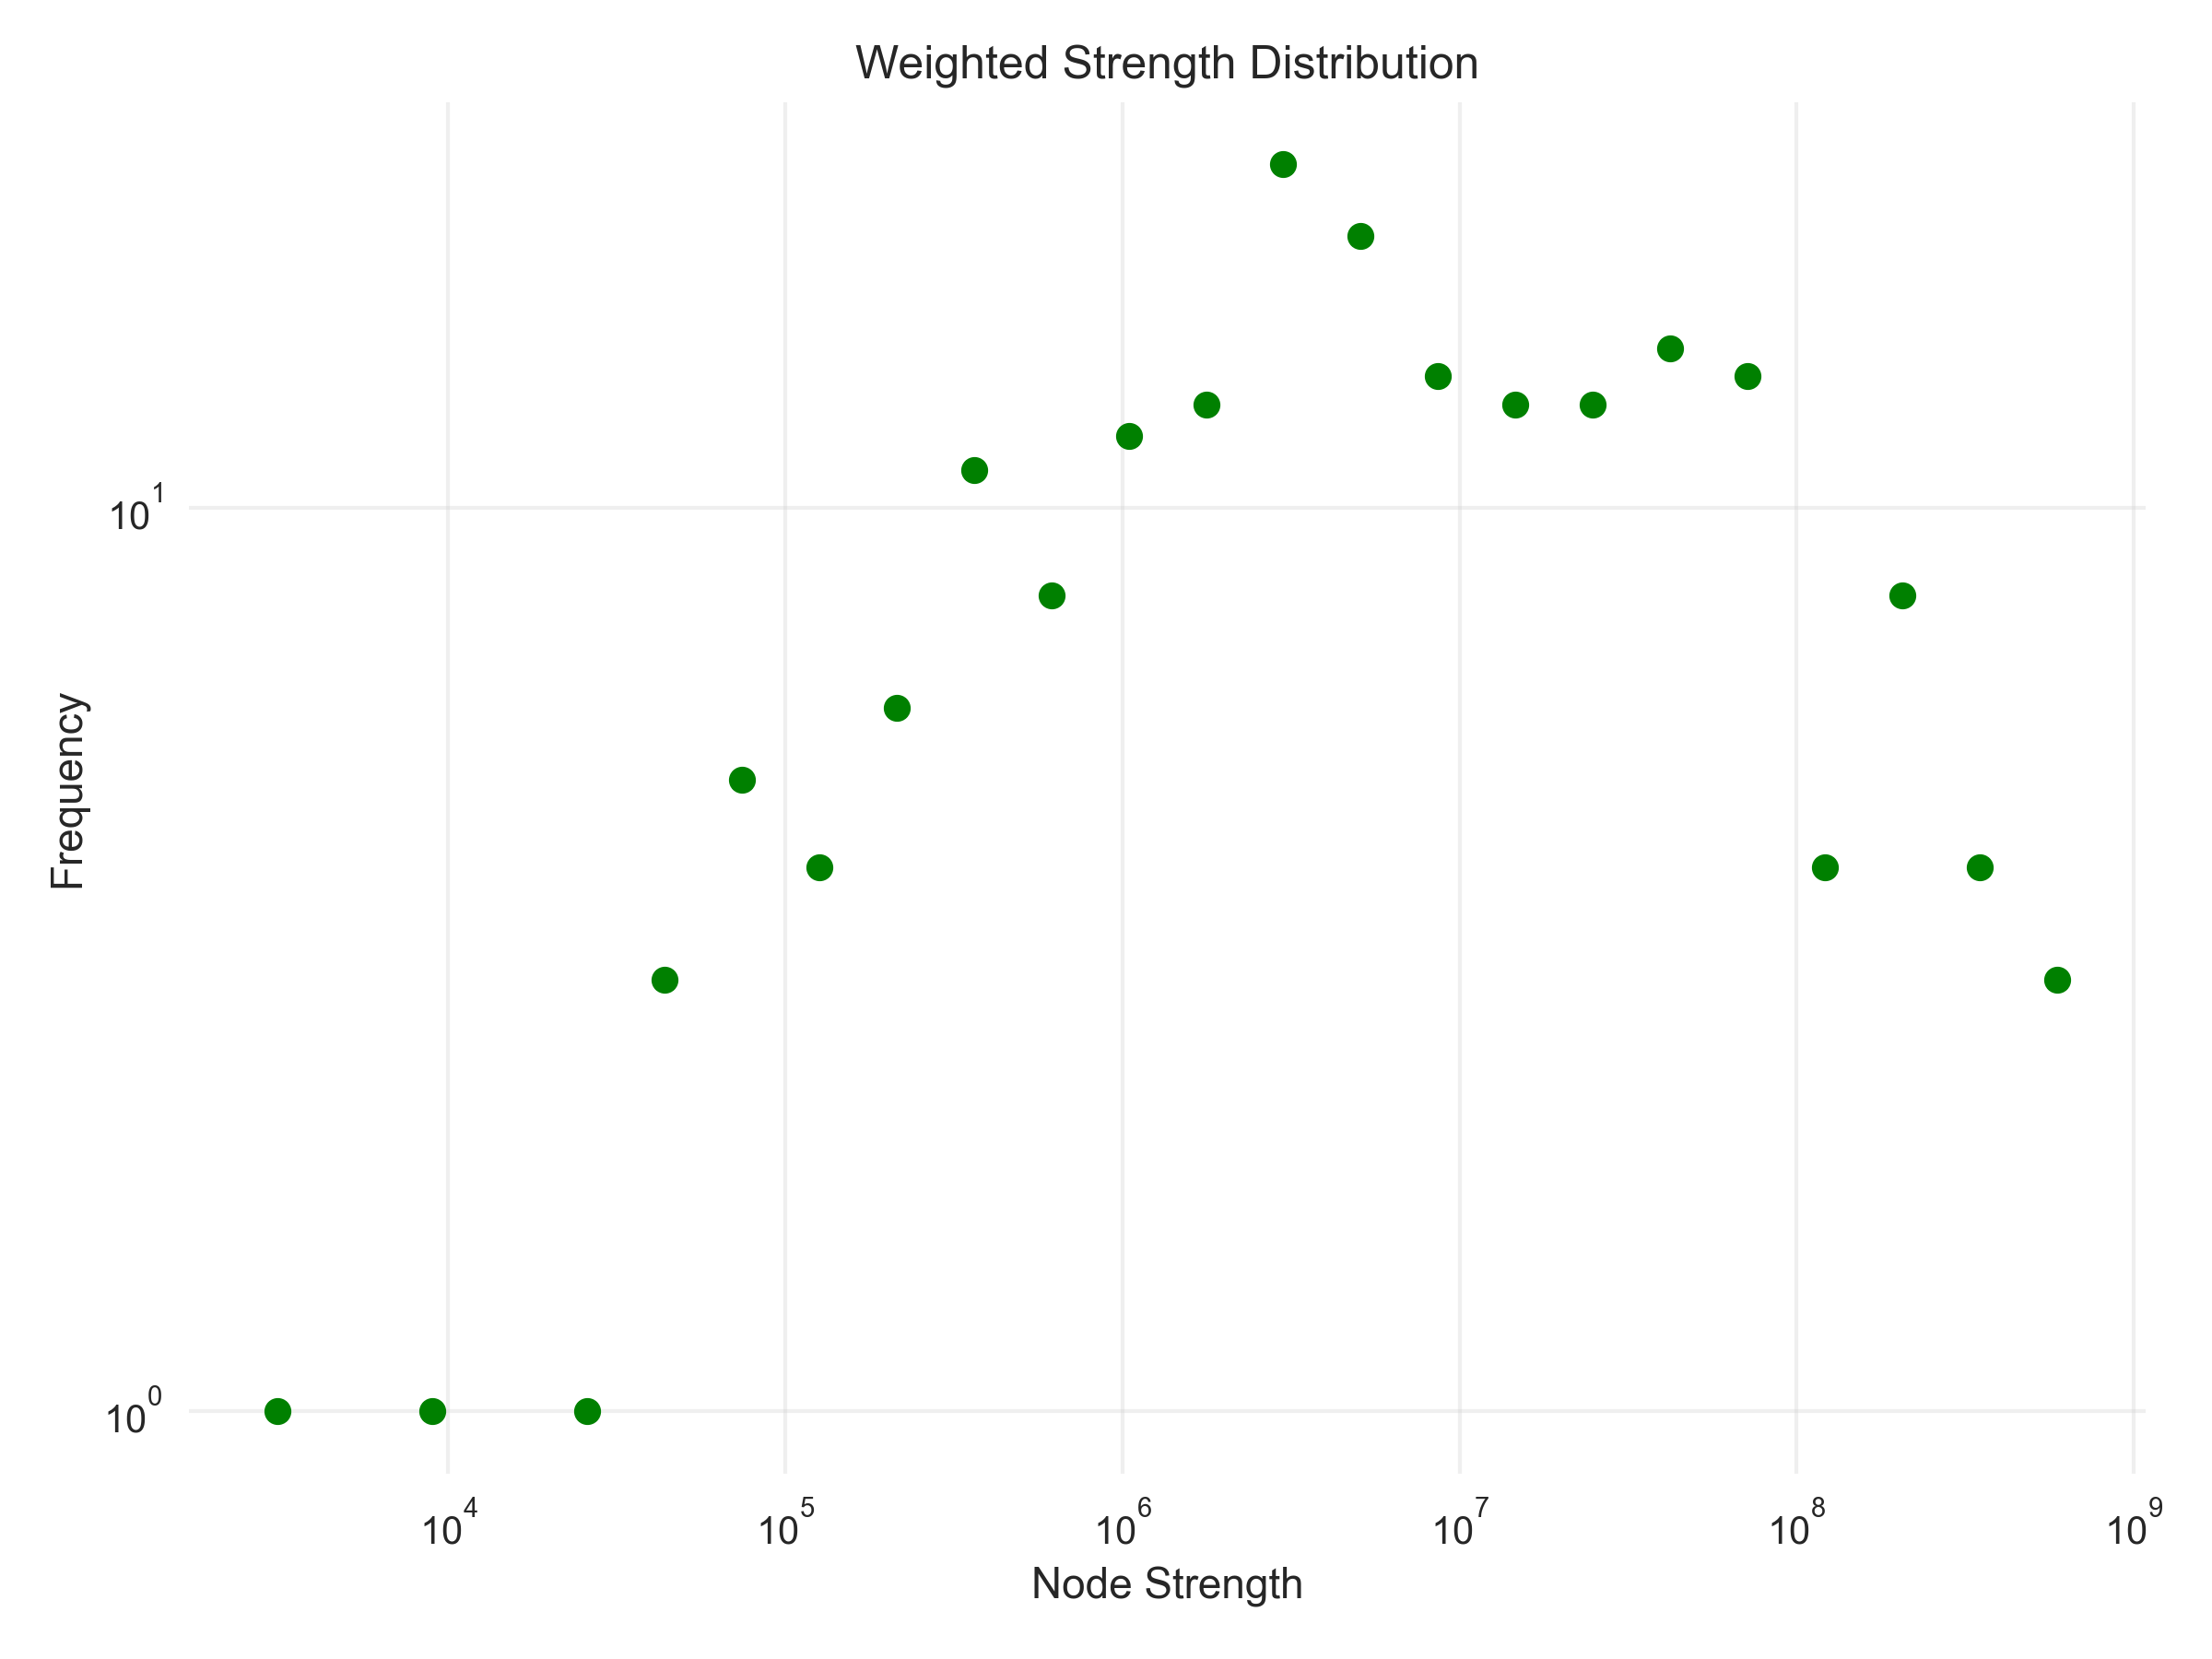
\includegraphics[width=\linewidth]{28_strength_hist_loglog.png}
    \caption{Strength distribution (log--log).}
  \end{subfigure}
  \caption{Connectivity and trade-value strength exhibit heavy tails: most countries are moderate, a small tail is extreme.}
  \label{fig:heavy-tail-hists}
\end{figure}

\begin{figure}[H]
  \centering
  \begin{subfigure}[t]{0.49\linewidth}
    \centering
    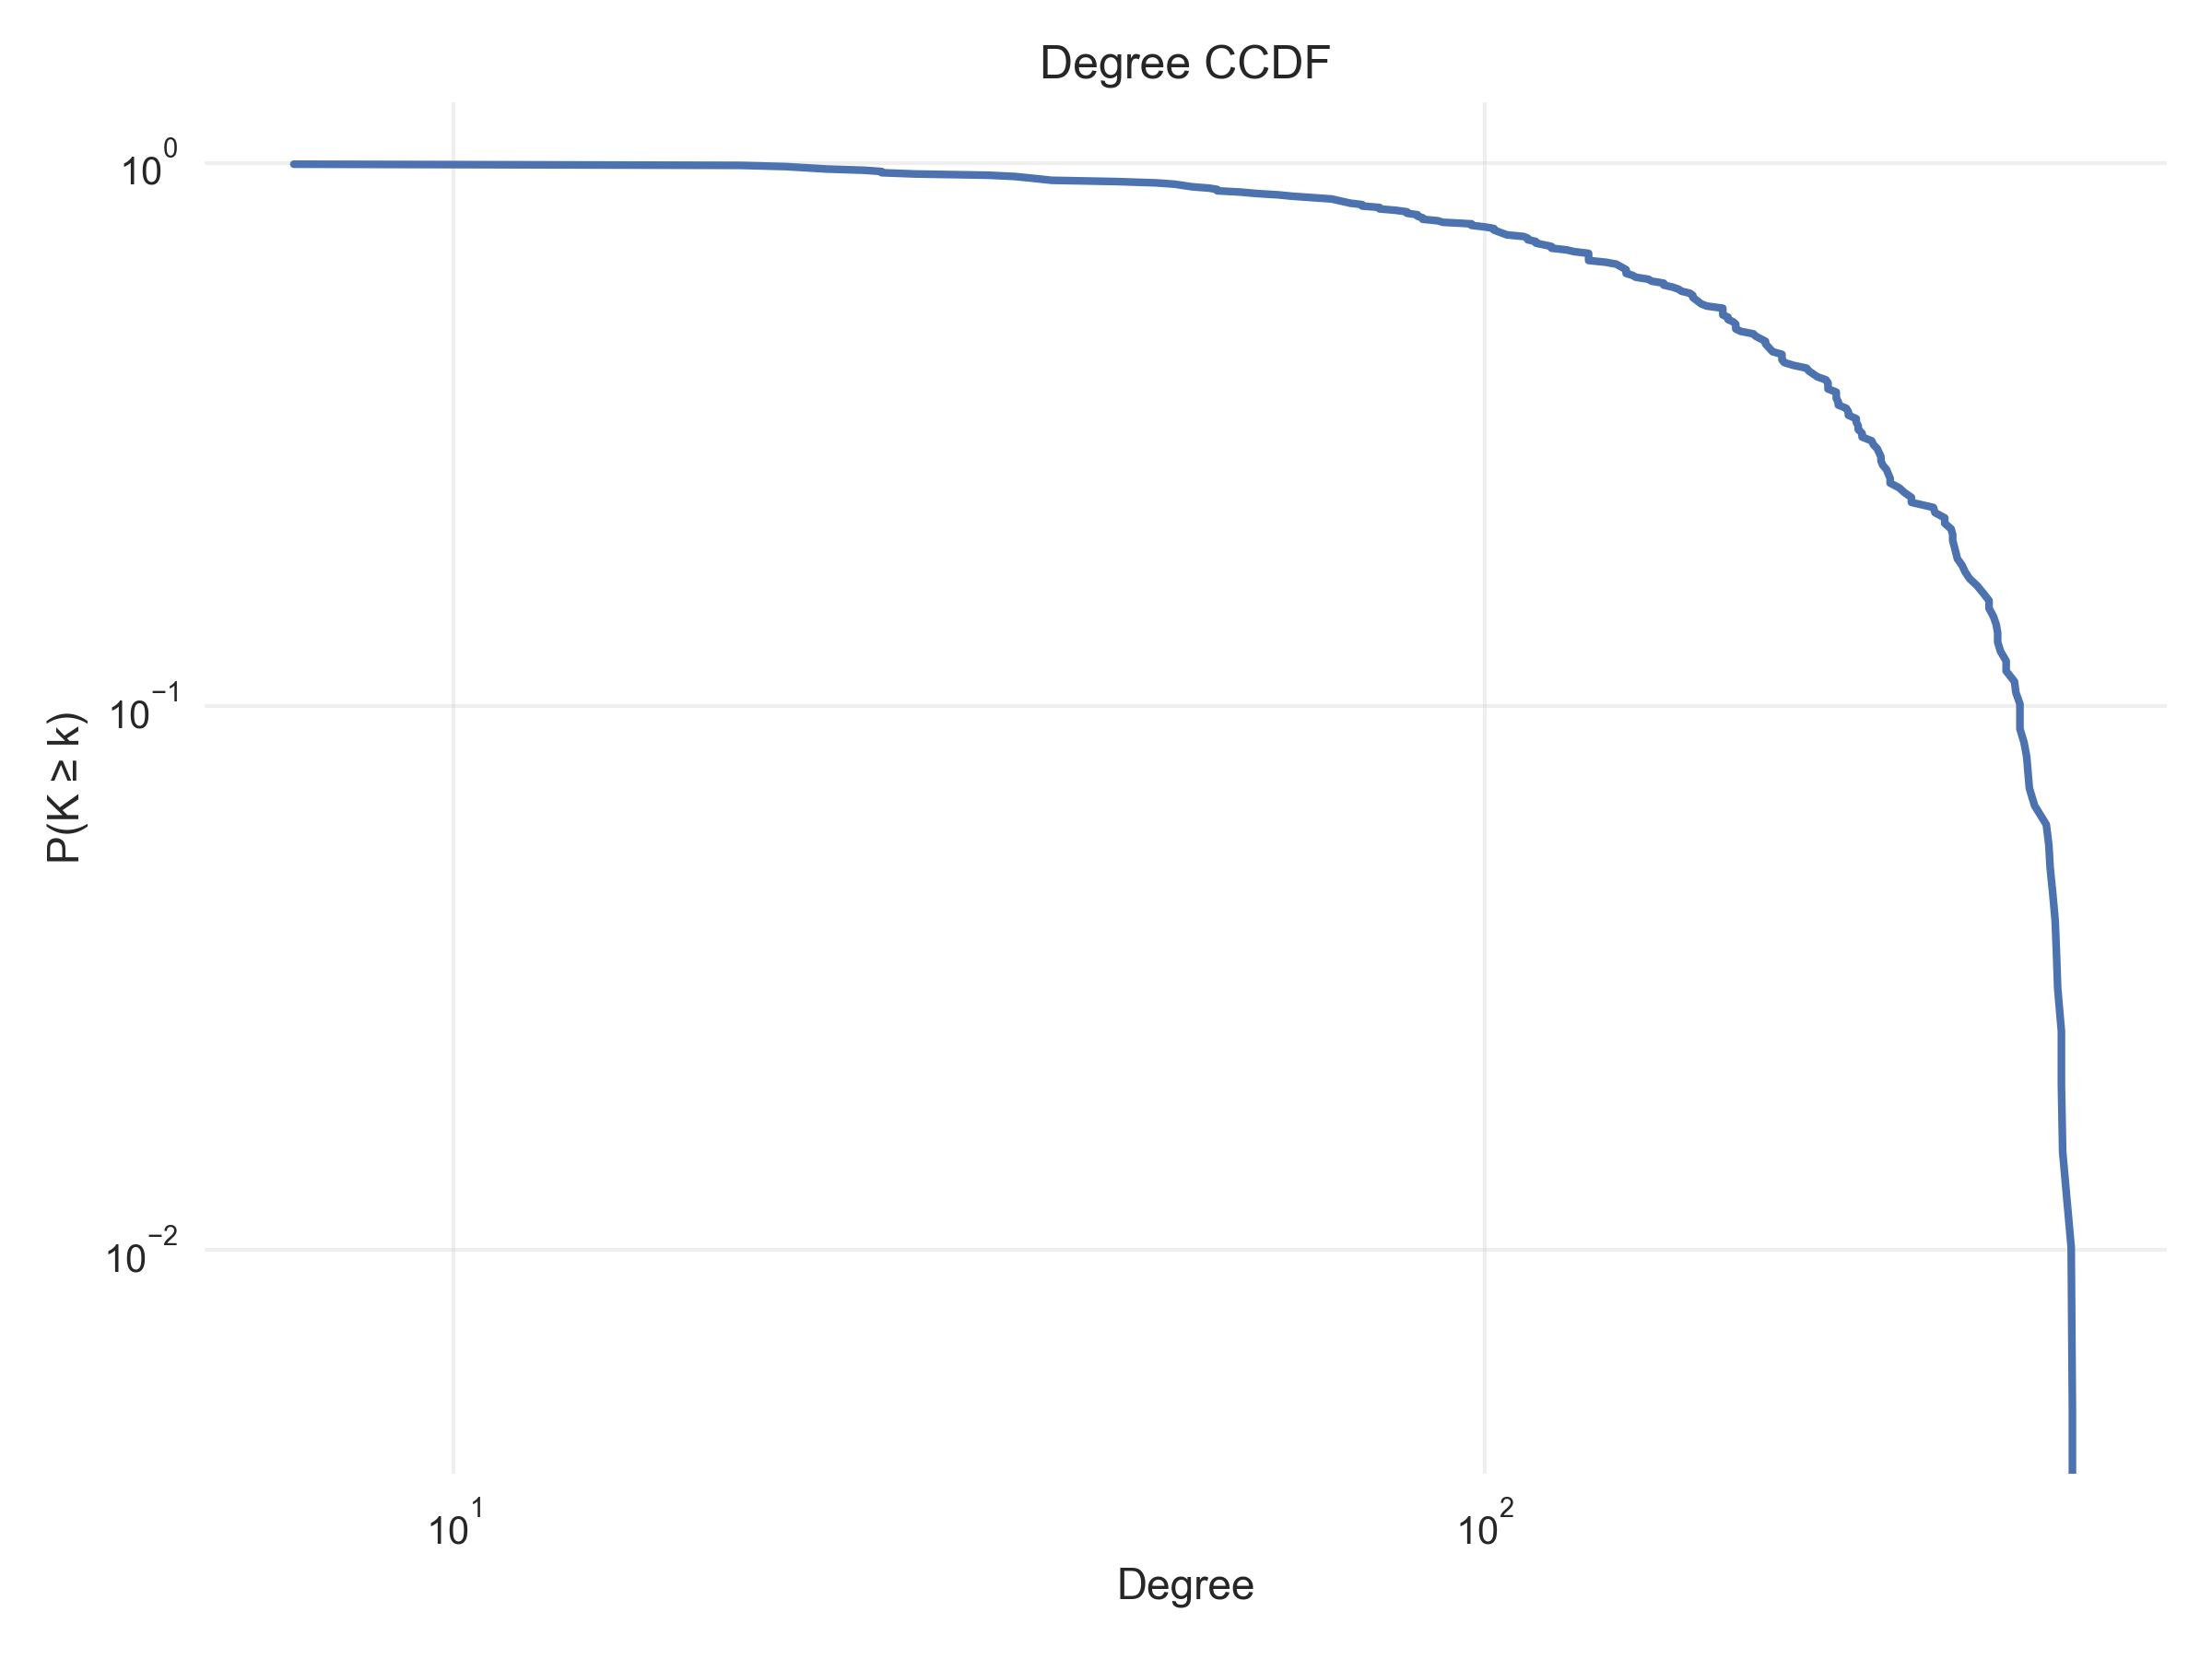
\includegraphics[width=\linewidth]{26_degree_ccdf.png}
    \caption{Degree CCDF (tail probability).}
  \end{subfigure}
  \hfill
  \begin{subfigure}[t]{0.49\linewidth}
    \centering
    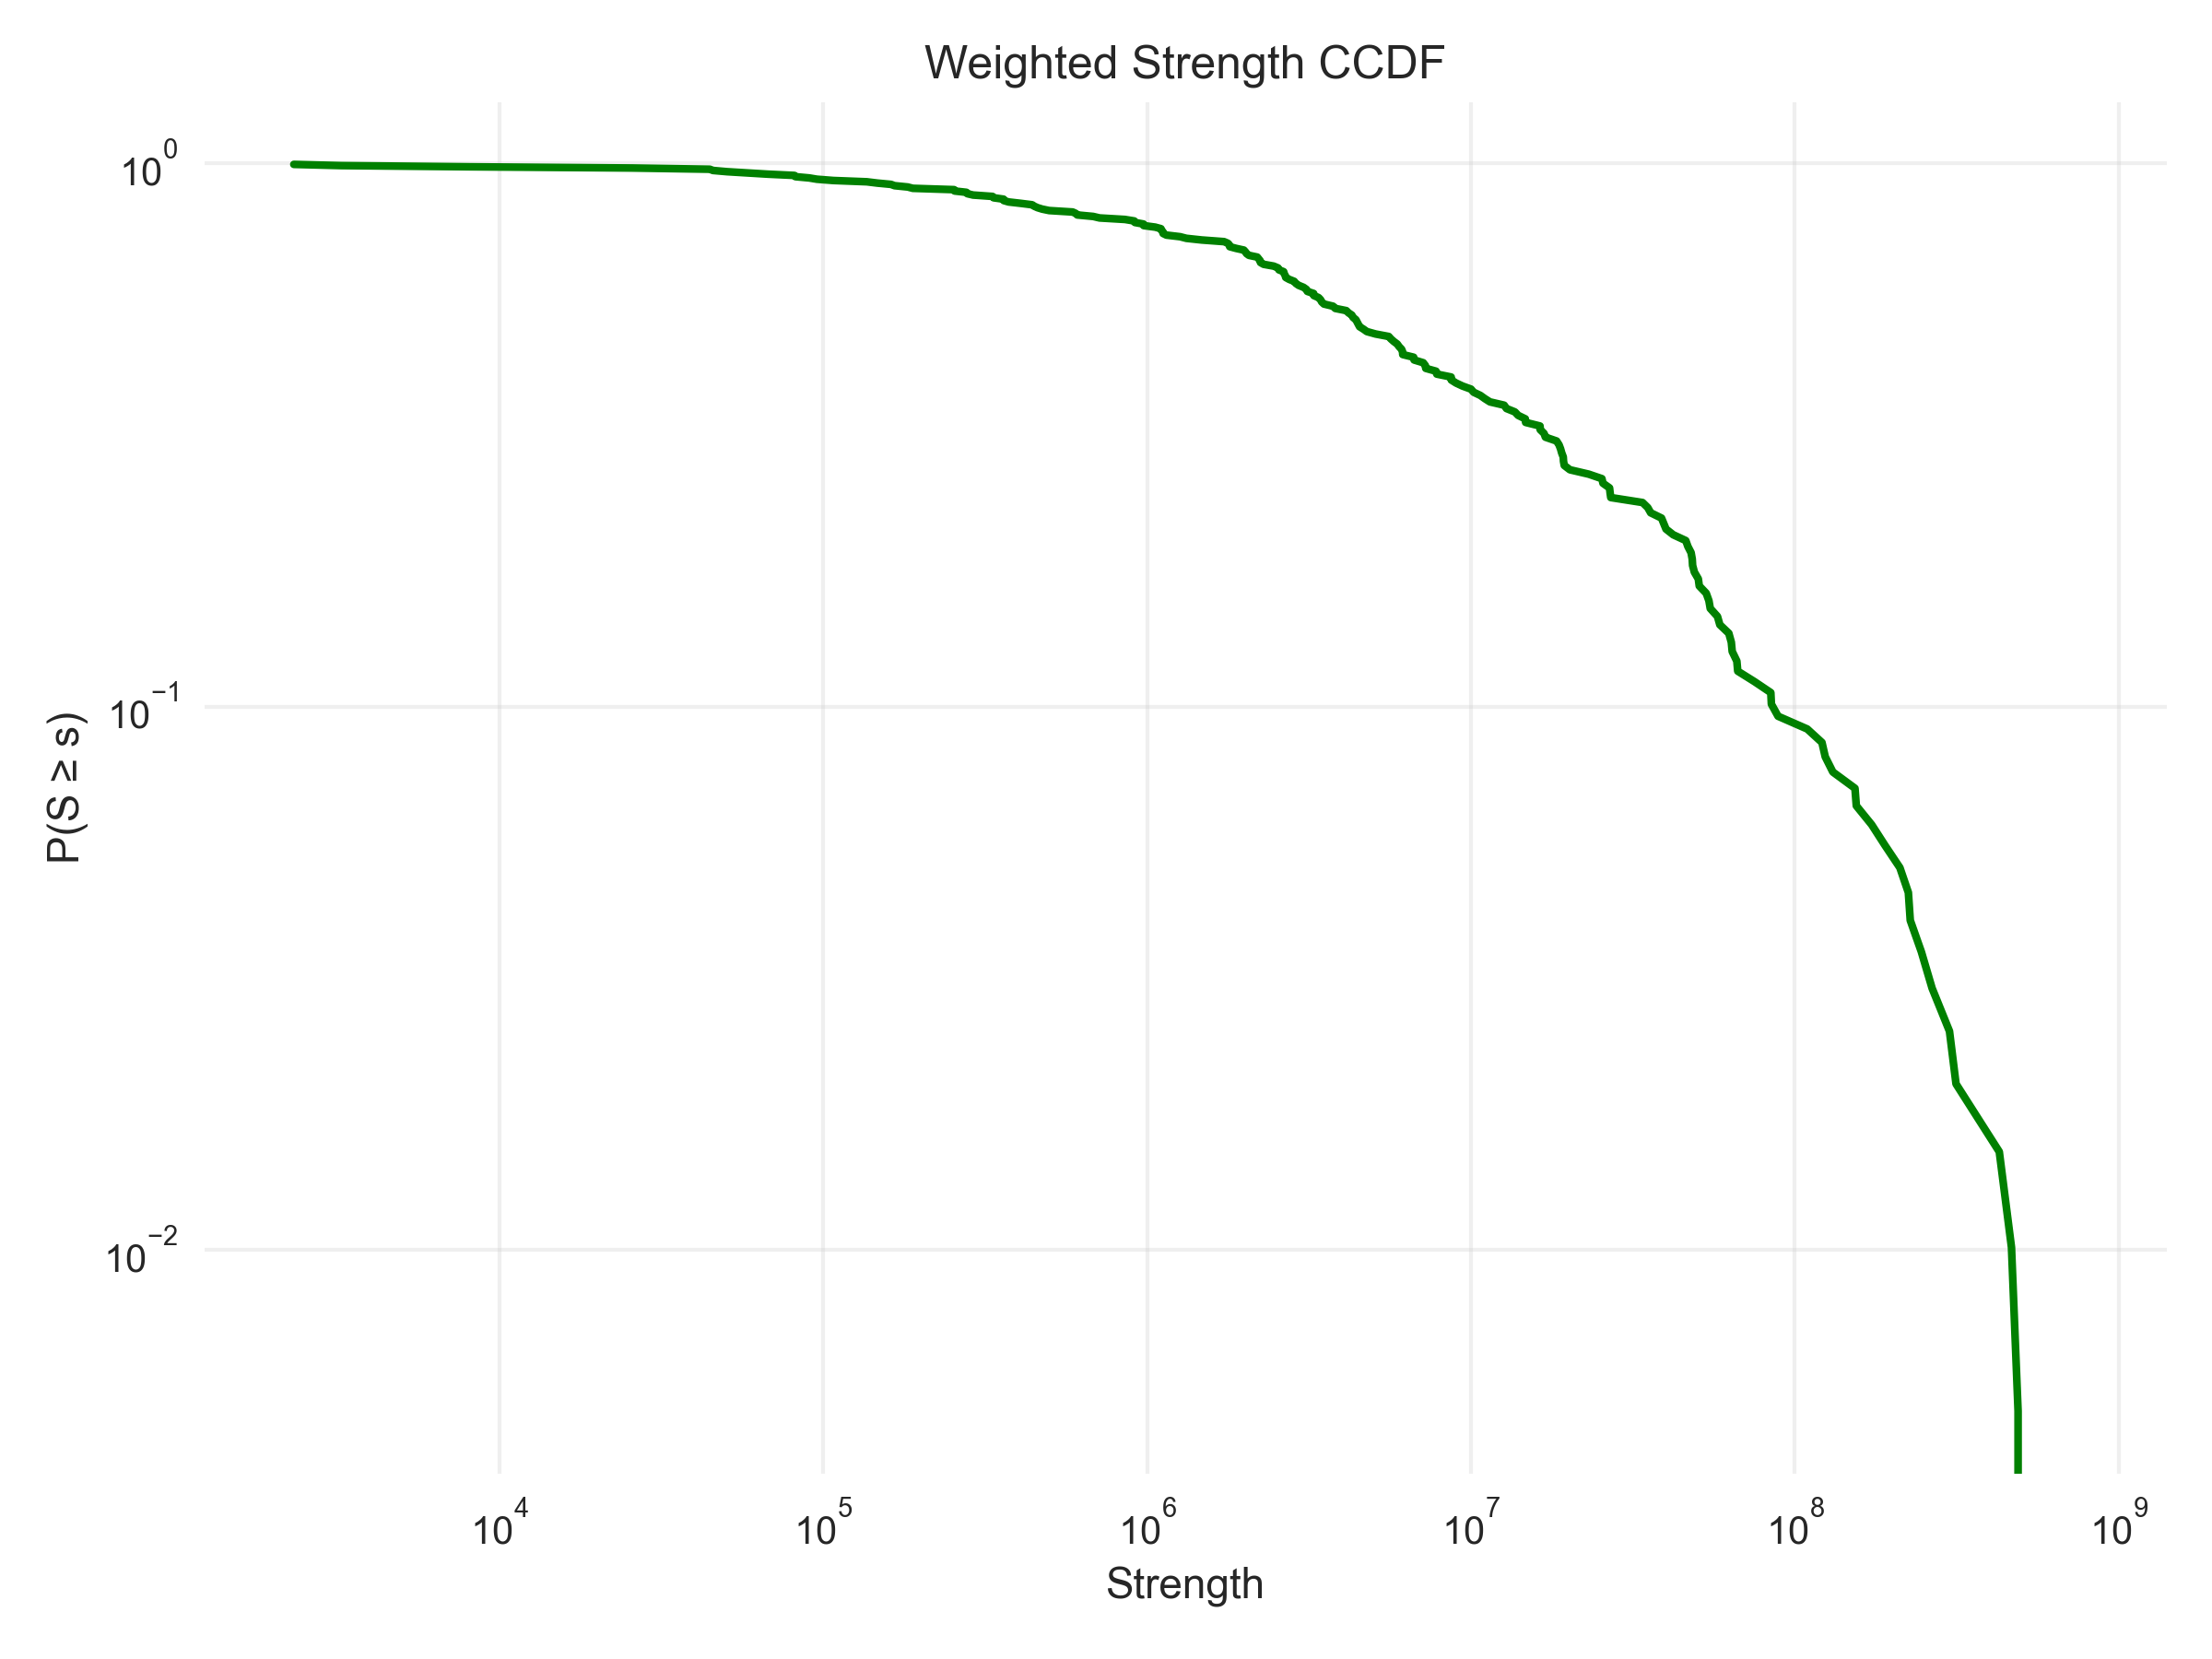
\includegraphics[width=\linewidth]{29_strength_ccdf.png}
    \caption{Strength CCDF (tail probability).}
  \end{subfigure}
  \caption{Complementary CDF views emphasize persistence of extreme hubs and high-flow nodes.}
  \label{fig:ccdfs}
\end{figure}

\subsection{Regional structure (communities)}
Community structure exists but is relatively weak in the unweighted topology (modularity $\approx 0.051$). Weighted communities better reflect high-volume blocs.

\begin{figure}[H]
  \centering
  \begin{subfigure}[t]{0.49\linewidth}
    \centering
    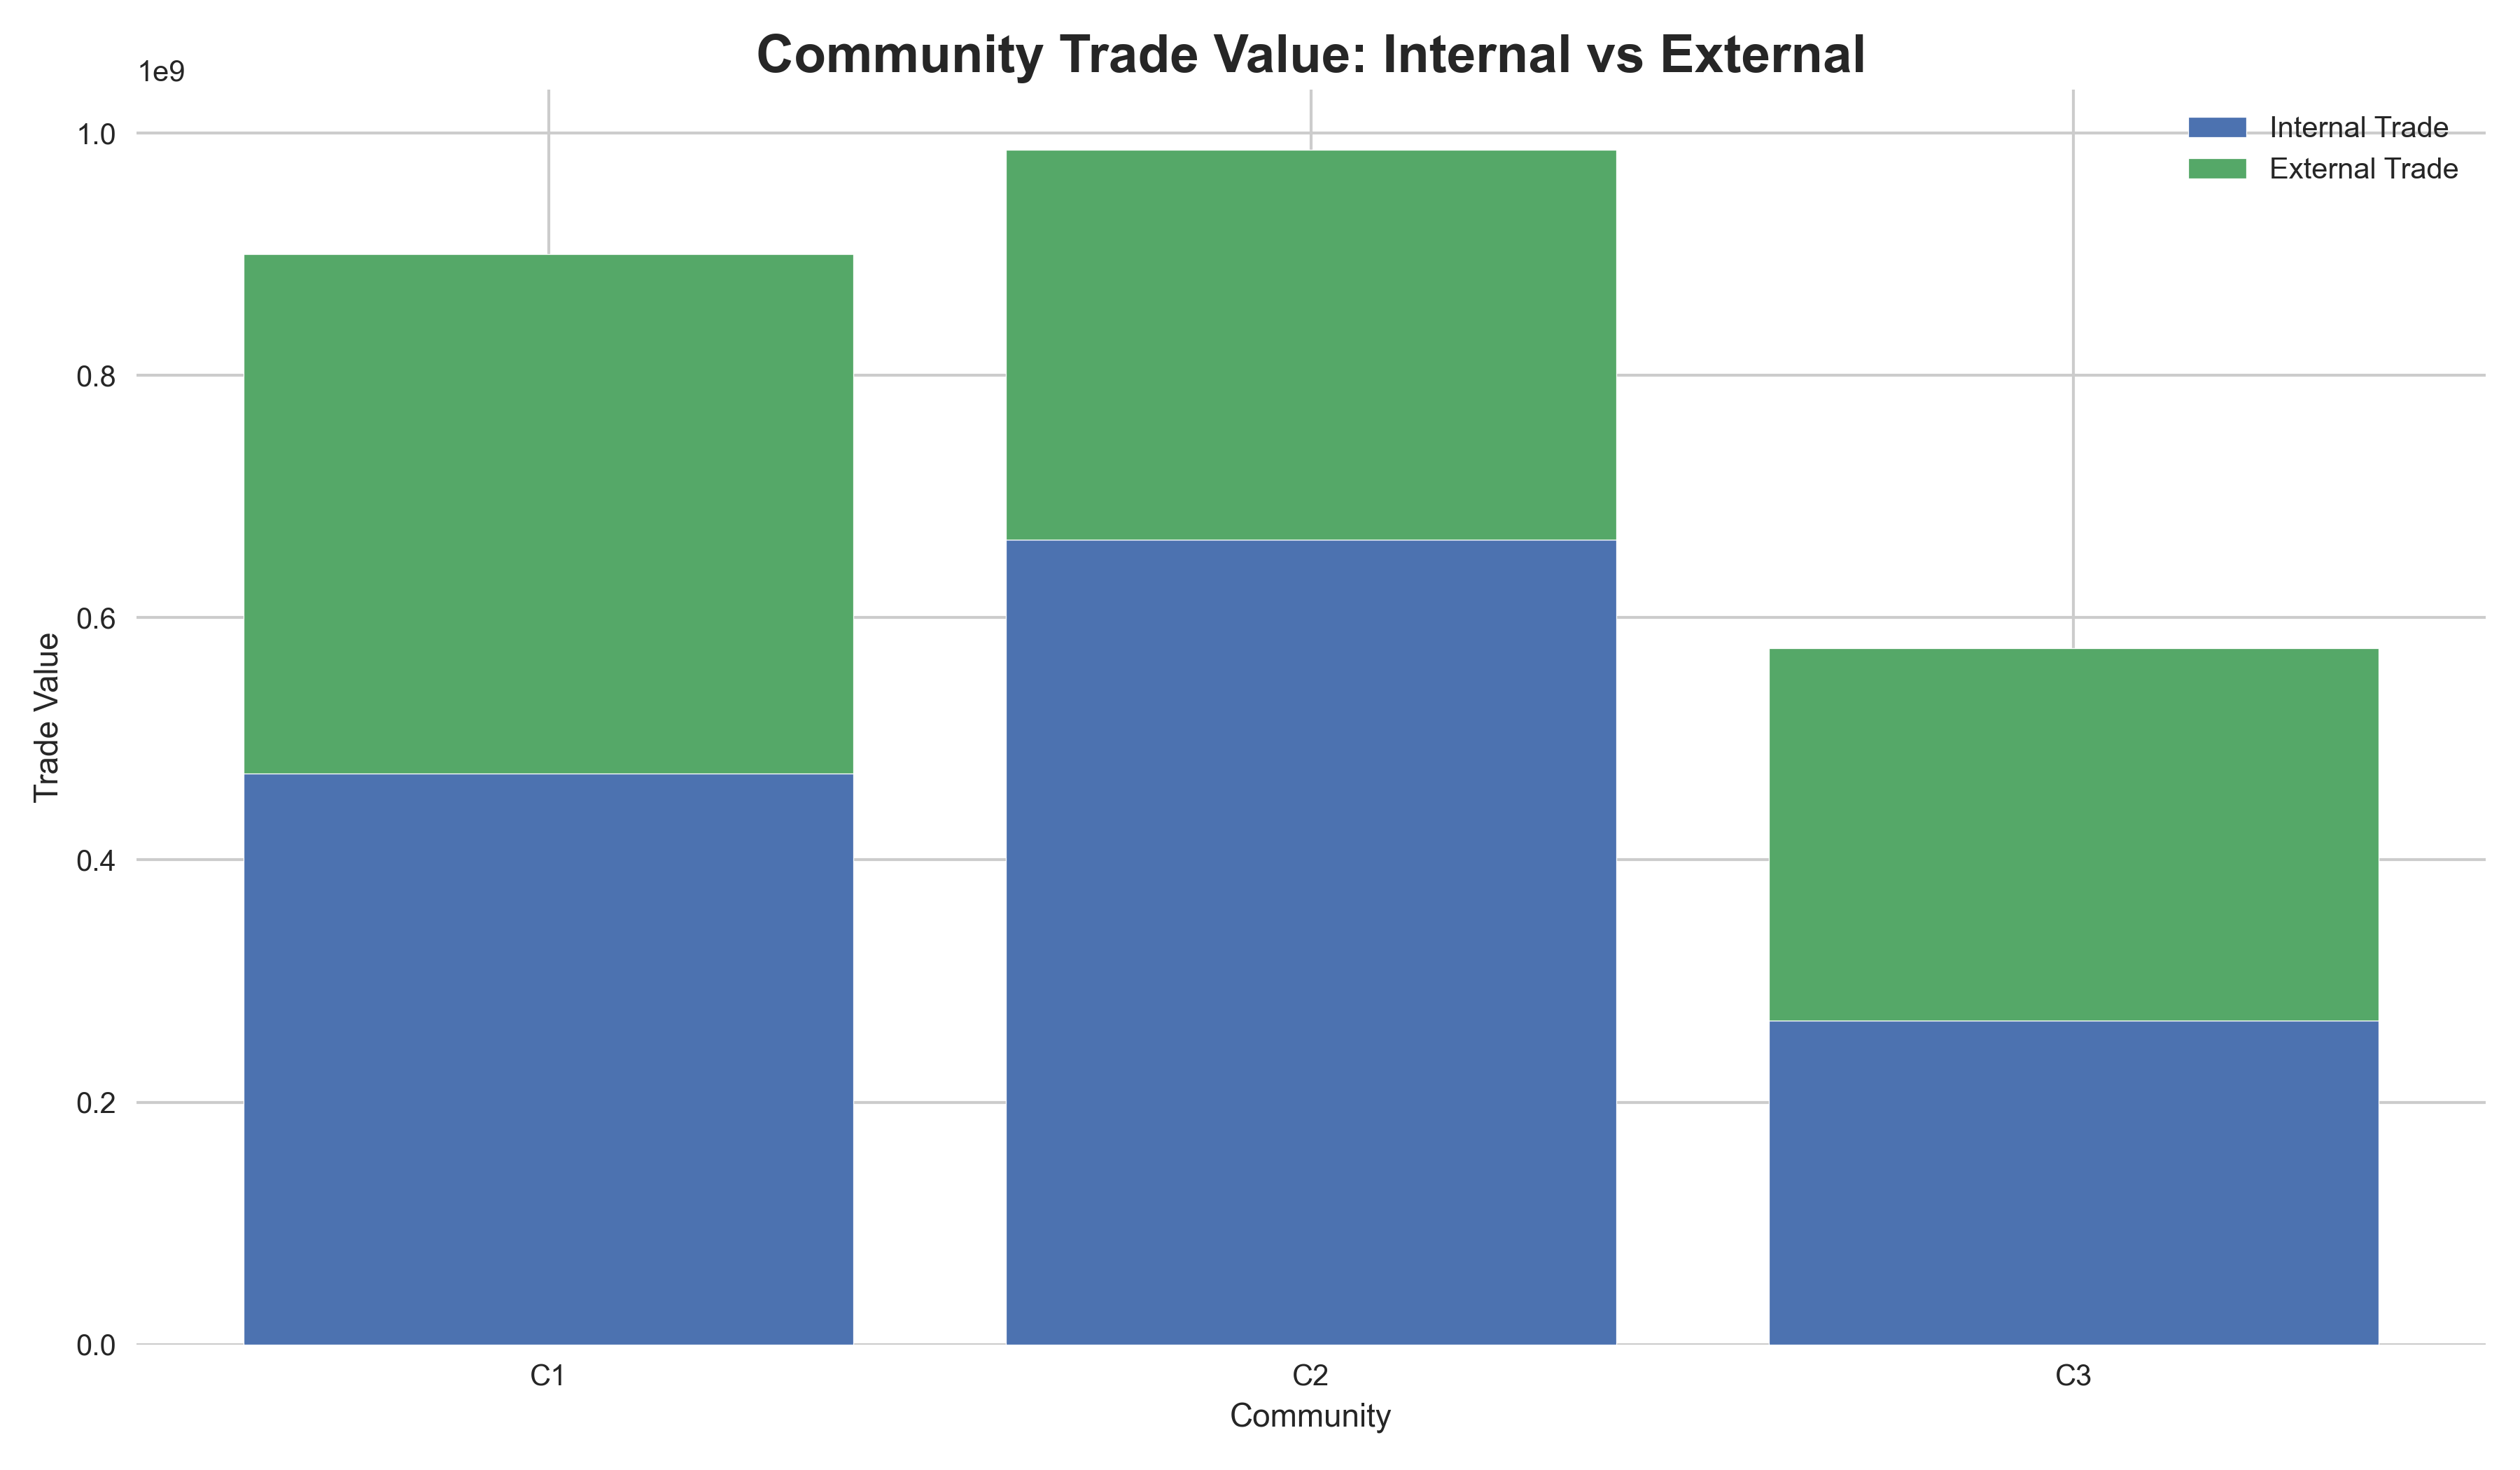
\includegraphics[width=\linewidth]{weighted_community_internal_external.png}
    \caption{Internal vs external trade by weighted communities.}
  \end{subfigure}
  \hfill
  \begin{subfigure}[t]{0.49\linewidth}
    \centering
    \includegraphics[width=\linewidth]{weighted_world_trade_communities_map.png}
    \caption{Weighted communities mapped geographically.}
  \end{subfigure}
  \caption{Volume-based community structure reveals trade blocs and dependency patterns.}
  \label{fig:communities}
\end{figure}

\paragraph{Concentration insights.}
\begin{itemize}
  \item Connectivity and trade value are heavy-tailed: most nodes are not system-defining.
  \item A small set of high-degree/high-strength countries forms the backbone.
  \item Concentration improves efficiency but increases vulnerability to targeted disruption.
\end{itemize}

\section{Critical Edges: High-Value and High-Betweenness Corridors}
This section is edge-centric: which routes carry the most value, and which are structurally irreplaceable for maintaining connectivity.

\begin{figure}[H]
  \centering
  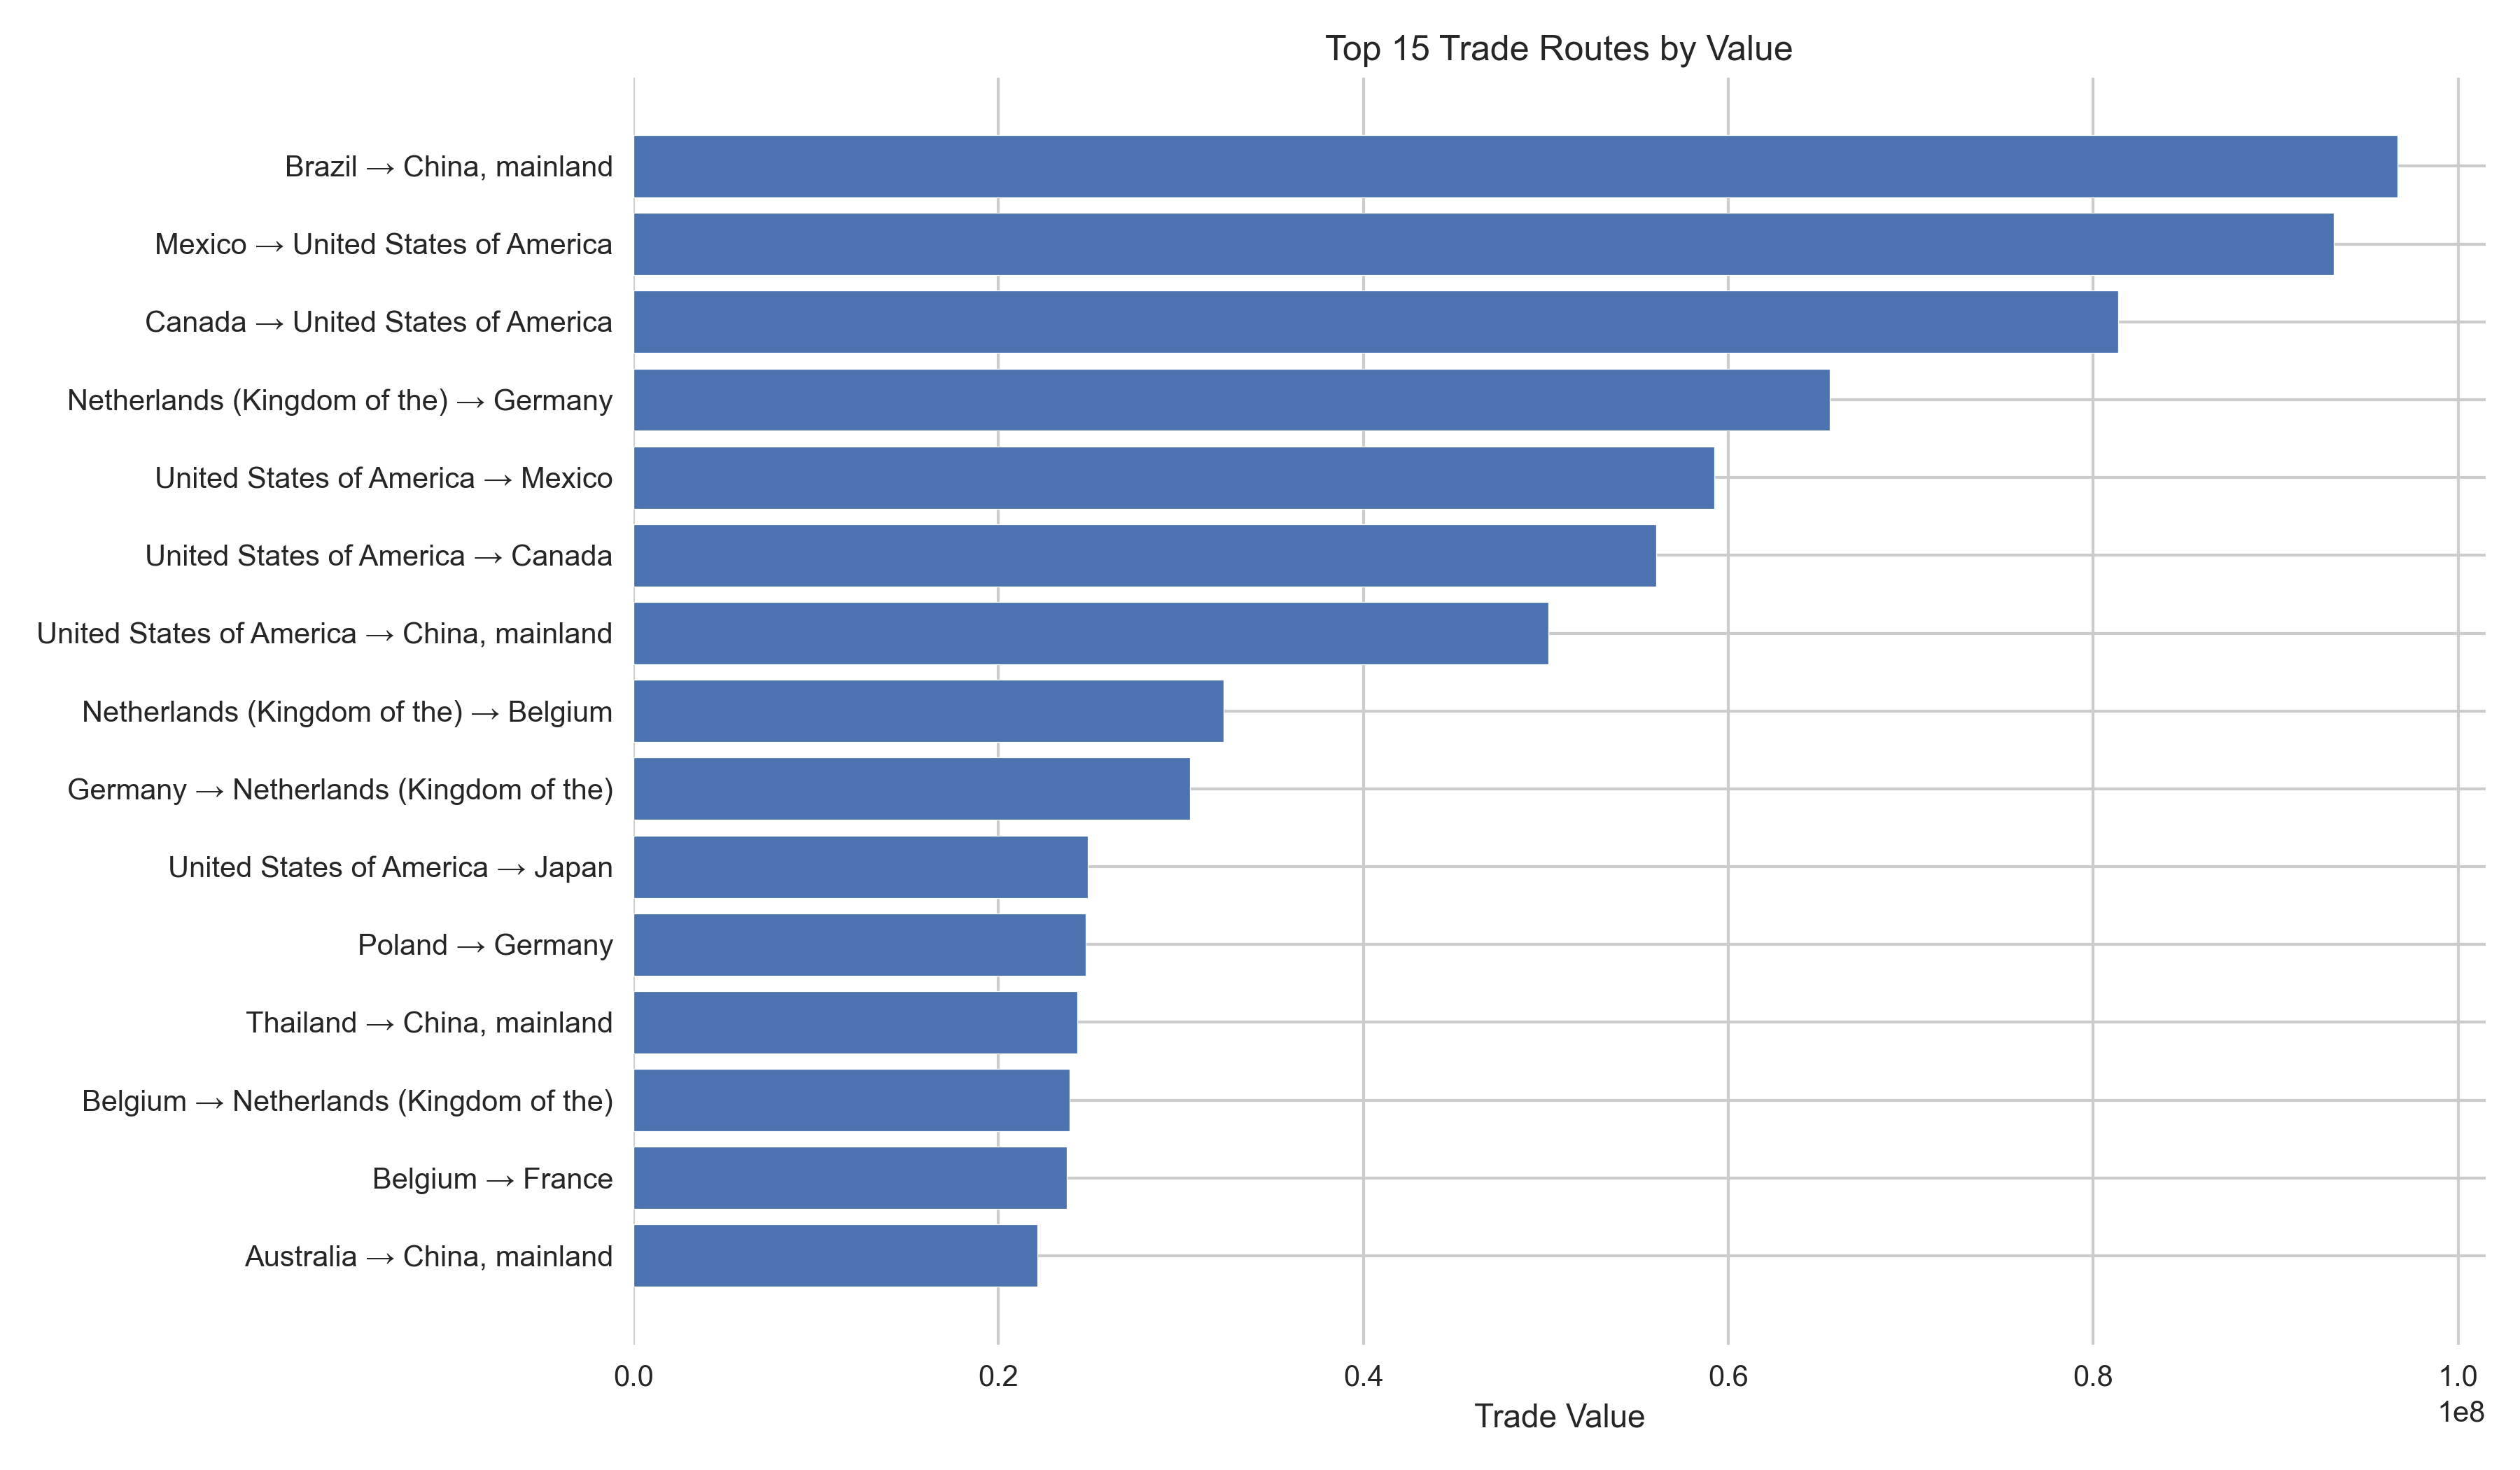
\includegraphics[width=0.98\linewidth]{02_top_trade_routes.png}
  \caption{Top trade routes by value: corridors with large immediate impact if disrupted.}
  \label{fig:top-routes}
\end{figure}

\subsection{Structural vs weighted criticality}
Structural criticality highlights bridges that preserve reachability; weighted criticality highlights corridors dominating total flow.

\begin{figure}[H]
  \centering
  \begin{subfigure}[t]{0.49\linewidth}
    \centering
    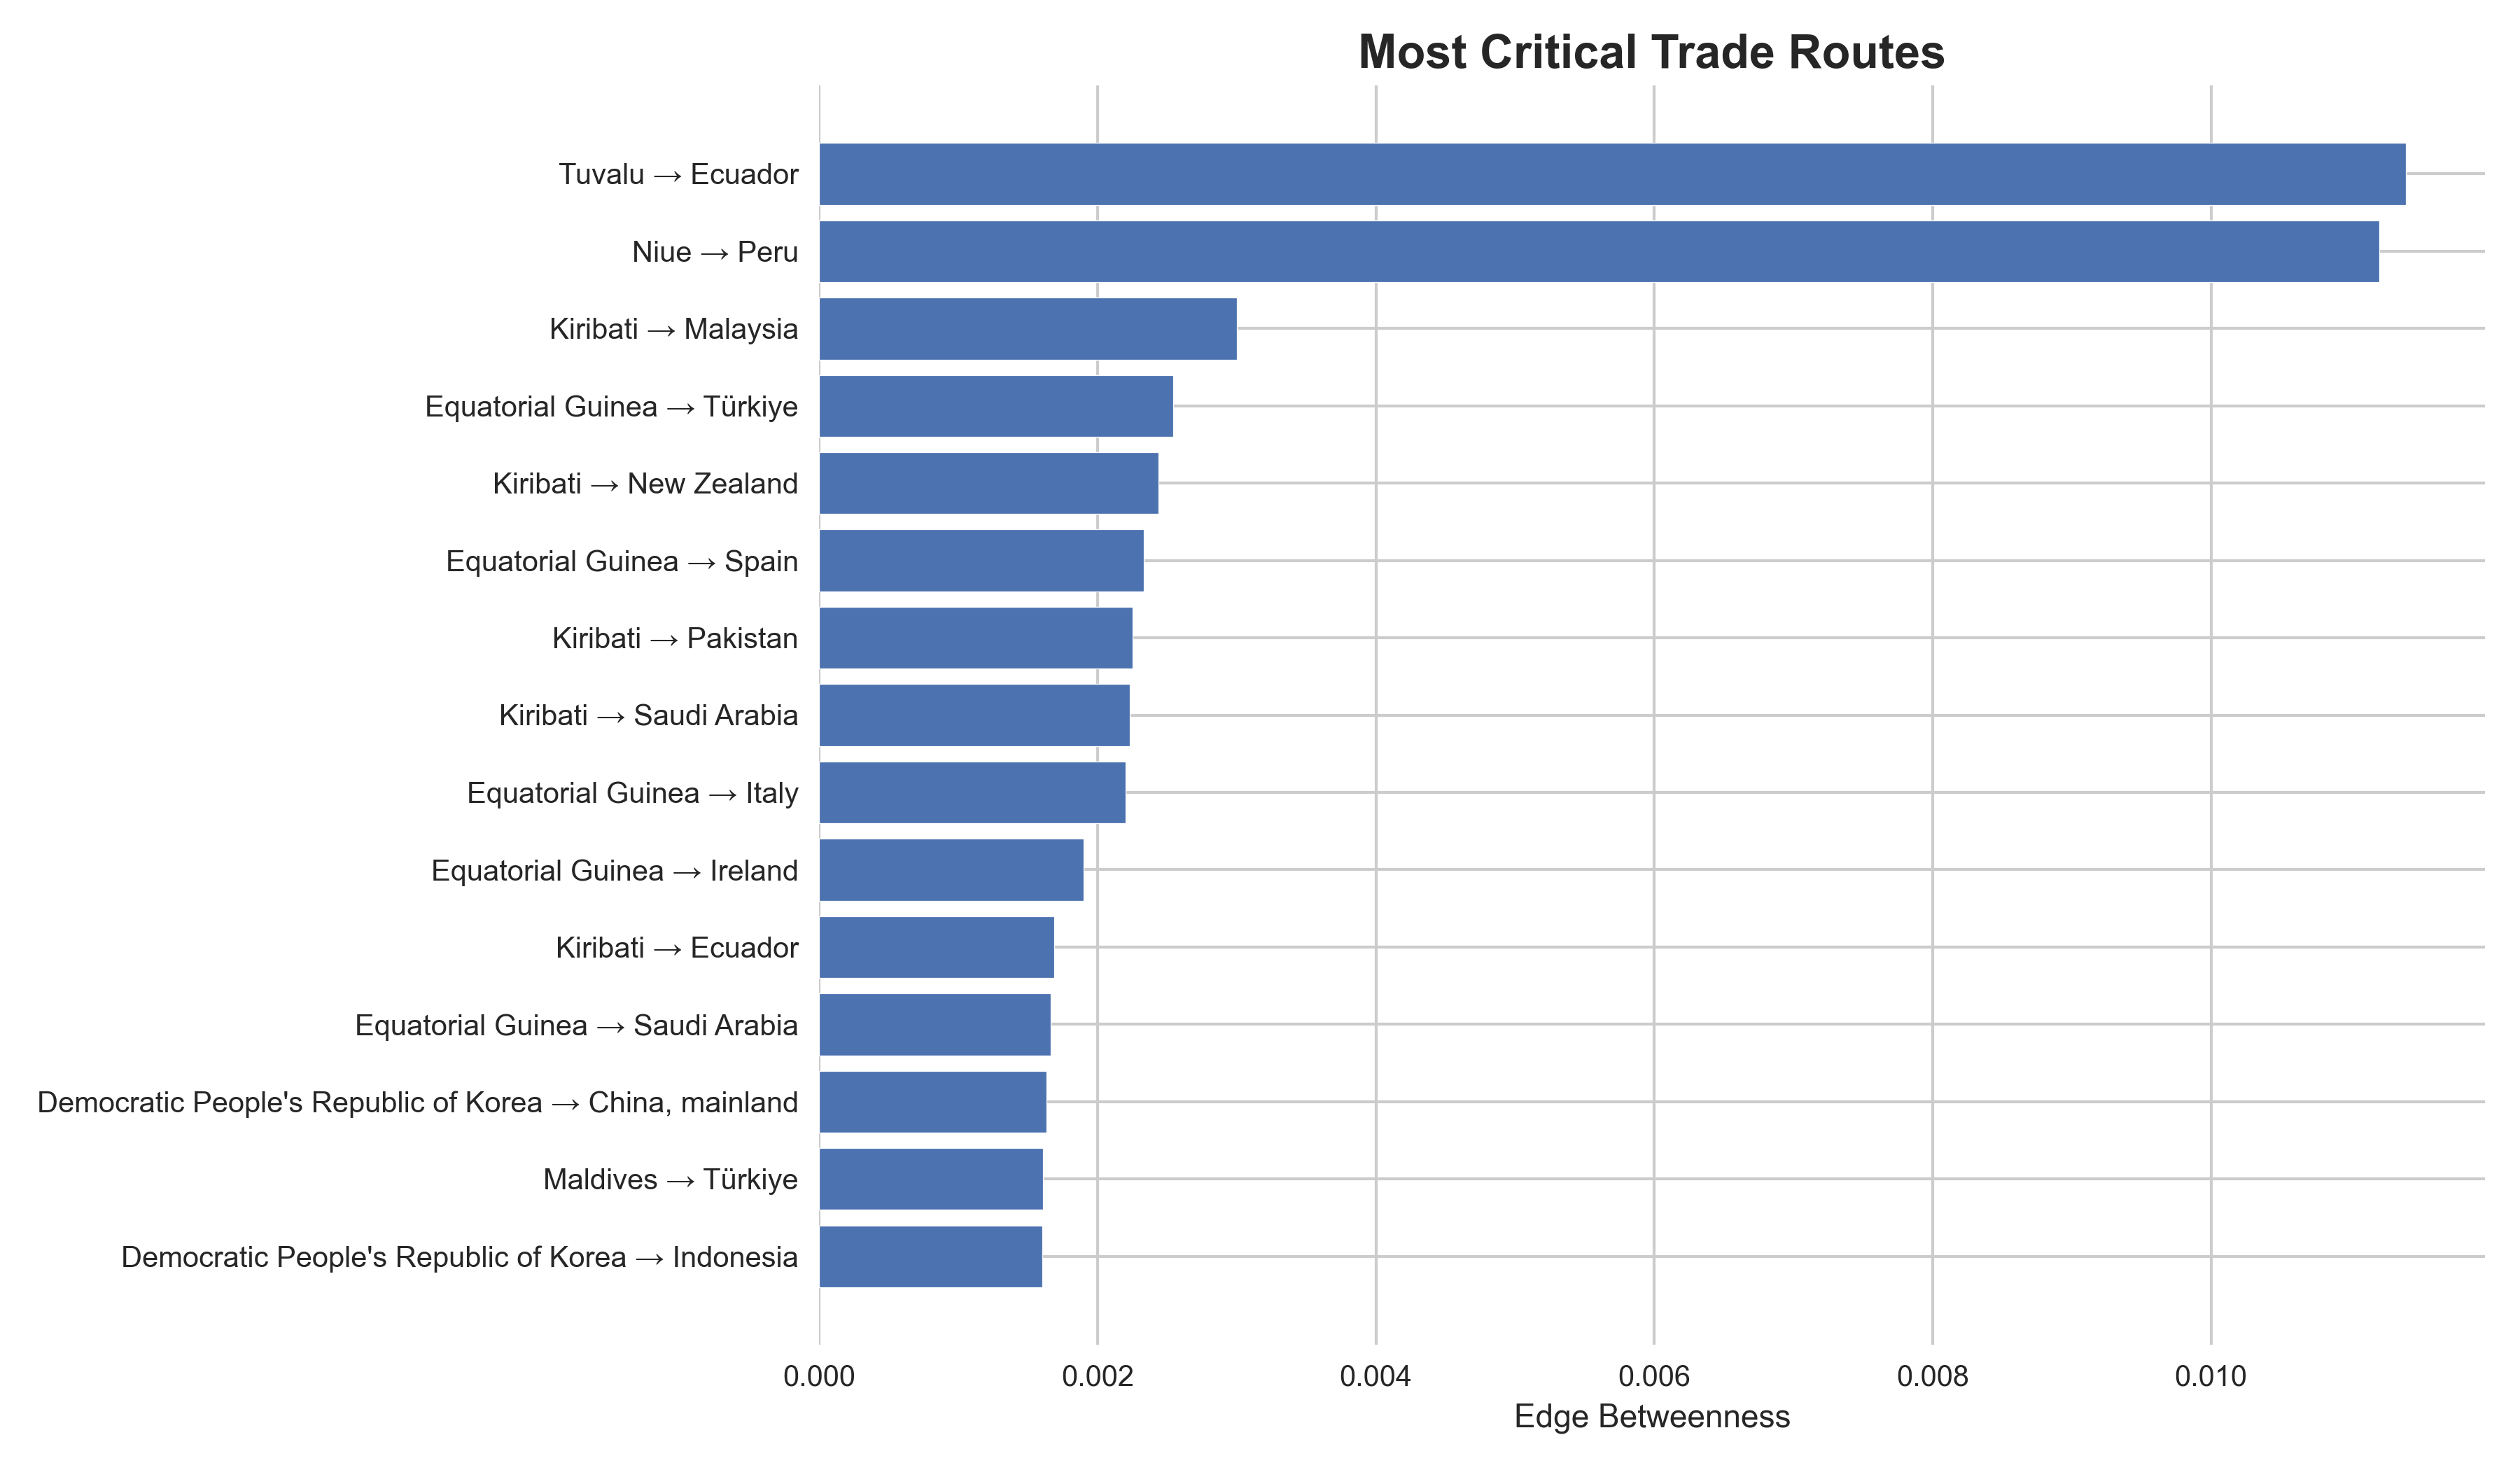
\includegraphics[width=\linewidth]{10_critical_routes.png}
    \caption{Structural critical routes (edge betweenness).}
  \end{subfigure}
  \hfill
  \begin{subfigure}[t]{0.49\linewidth}
    \centering
    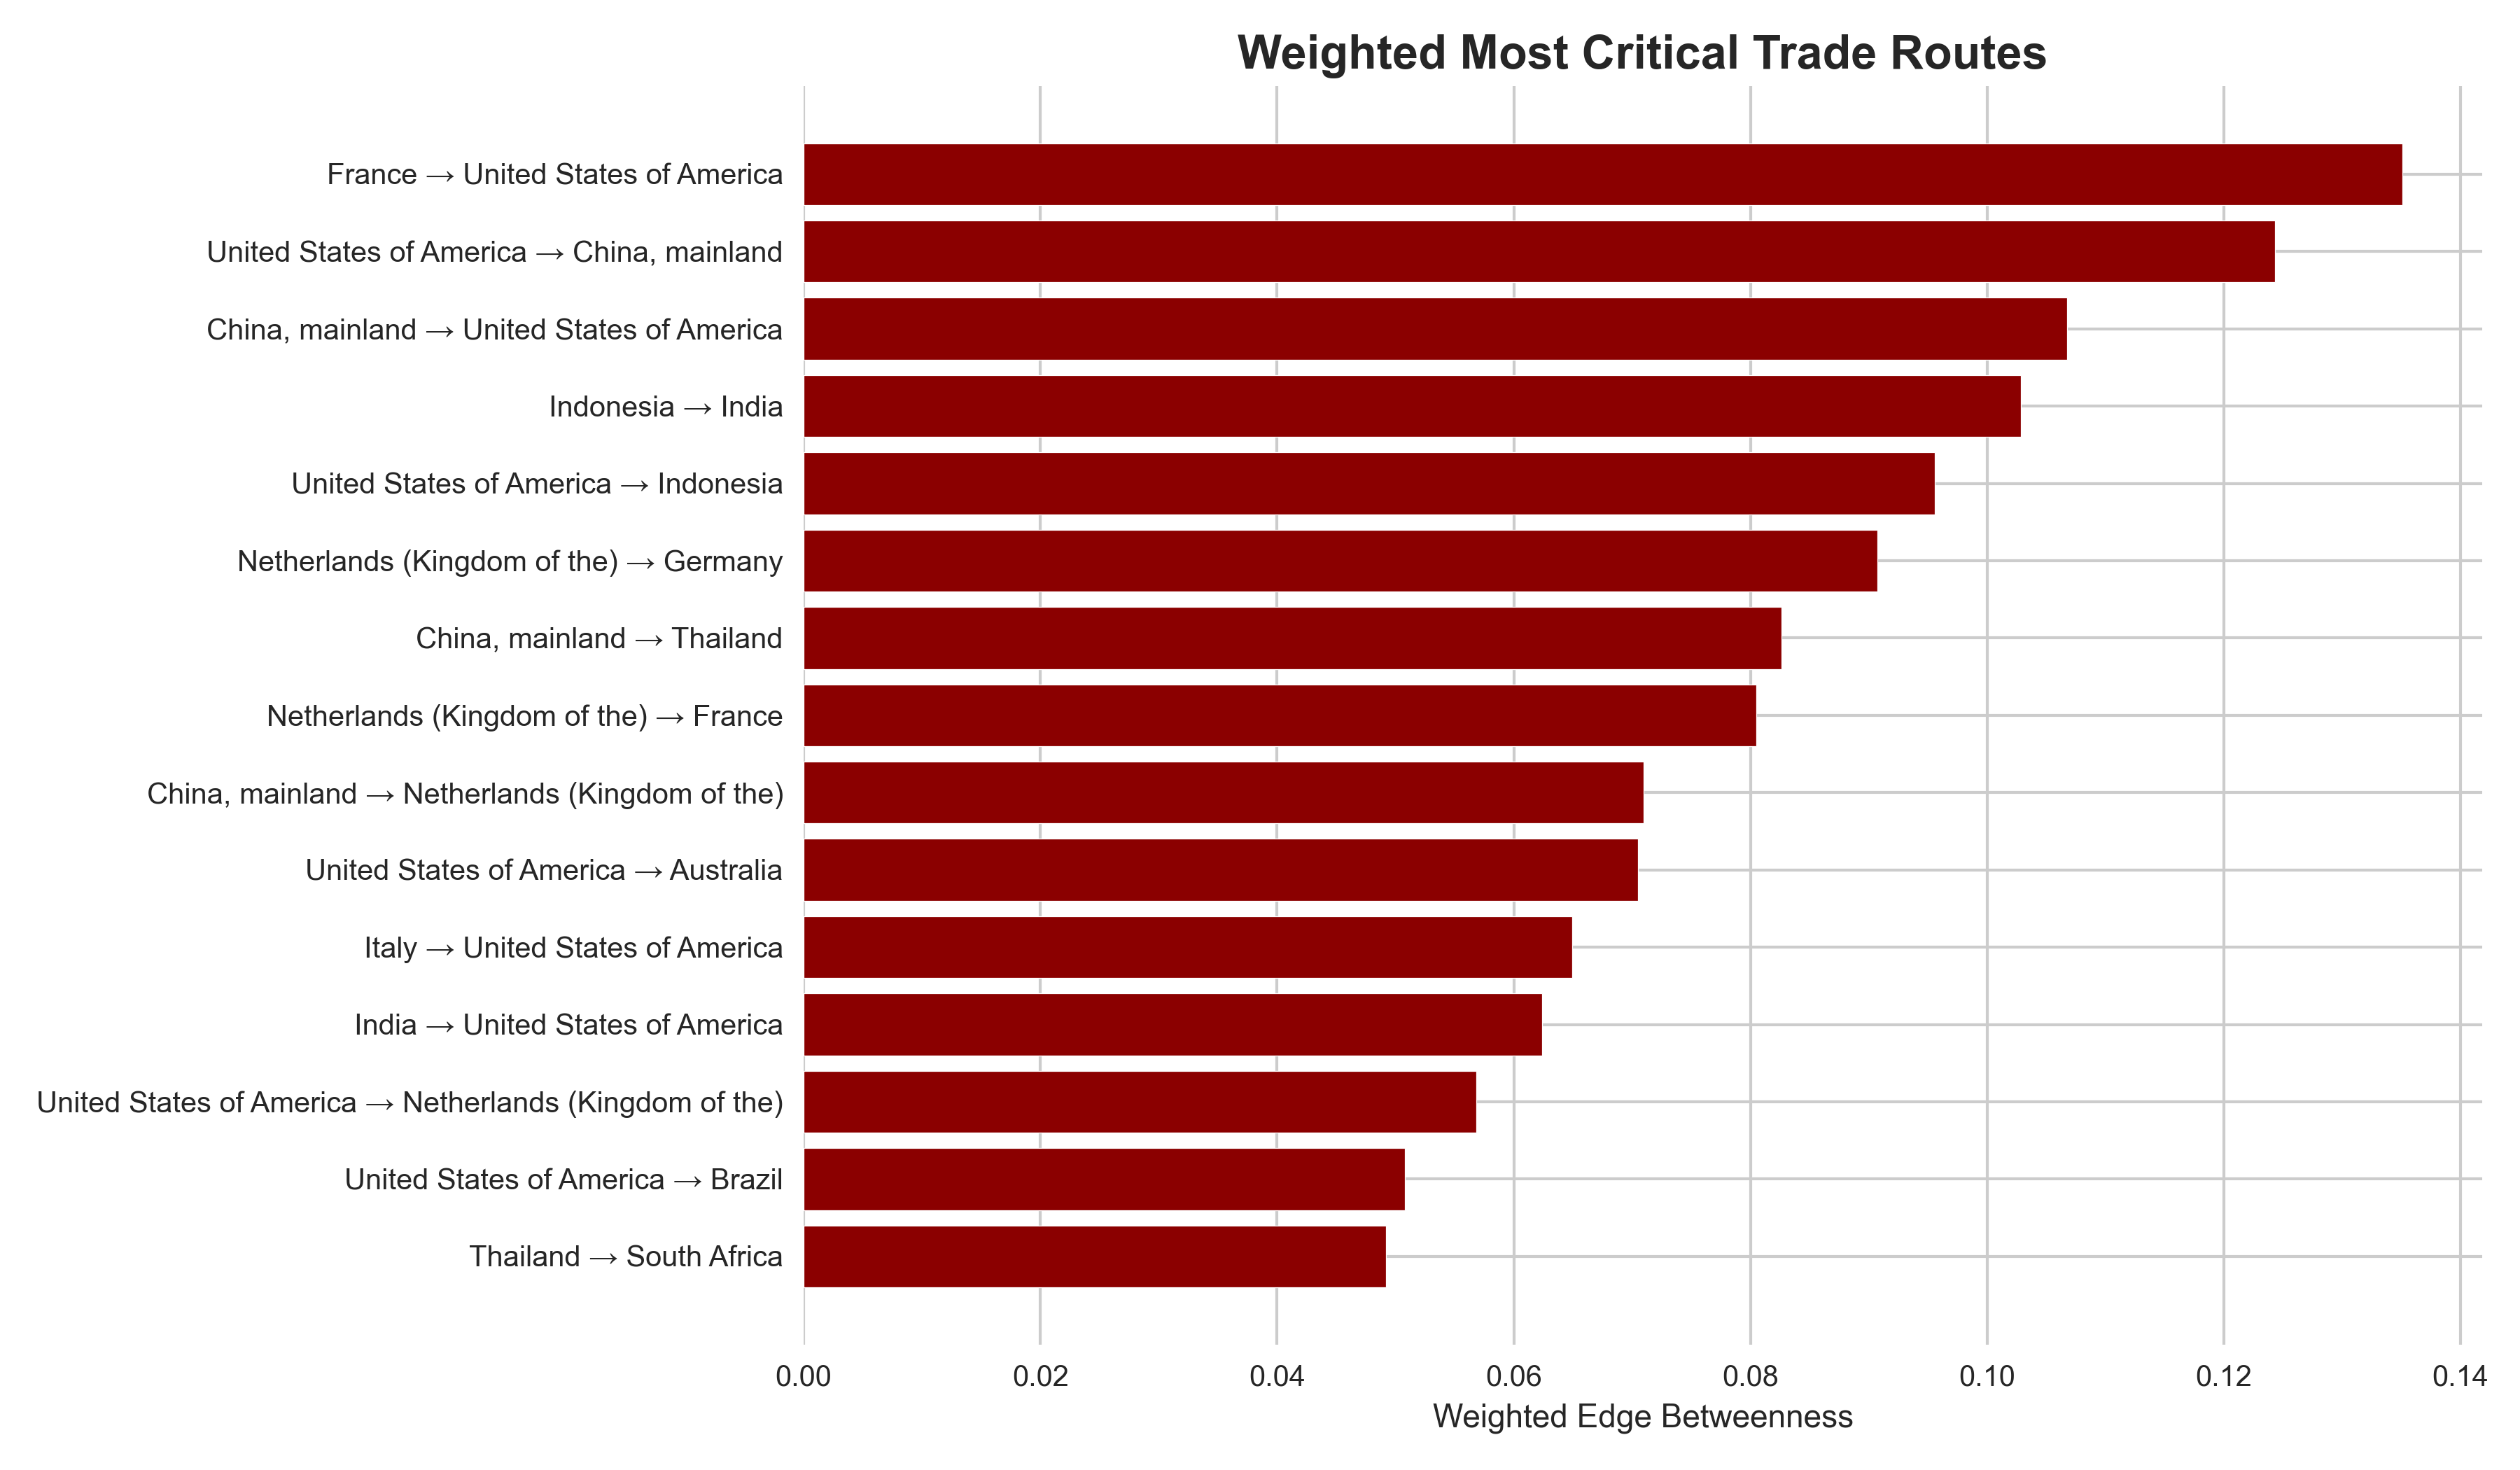
\includegraphics[width=\linewidth]{10b_weighted_critical_routes.png}
    \caption{Weighted critical routes (weighted edge betweenness).}
  \end{subfigure}
  \caption{Structural and weighted notions of edge criticality capture different risk channels.}
  \label{fig:critical-routes}
\end{figure}

\begin{figure}[H]
  \centering
  \begin{subfigure}[t]{0.49\linewidth}
    \centering
    \includegraphics[width=\linewidth]{11_highlighted_routes.png}
    \caption{Structural critical routes overlay.}
  \end{subfigure}
  \hfill
  \begin{subfigure}[t]{0.49\linewidth}
    \centering
    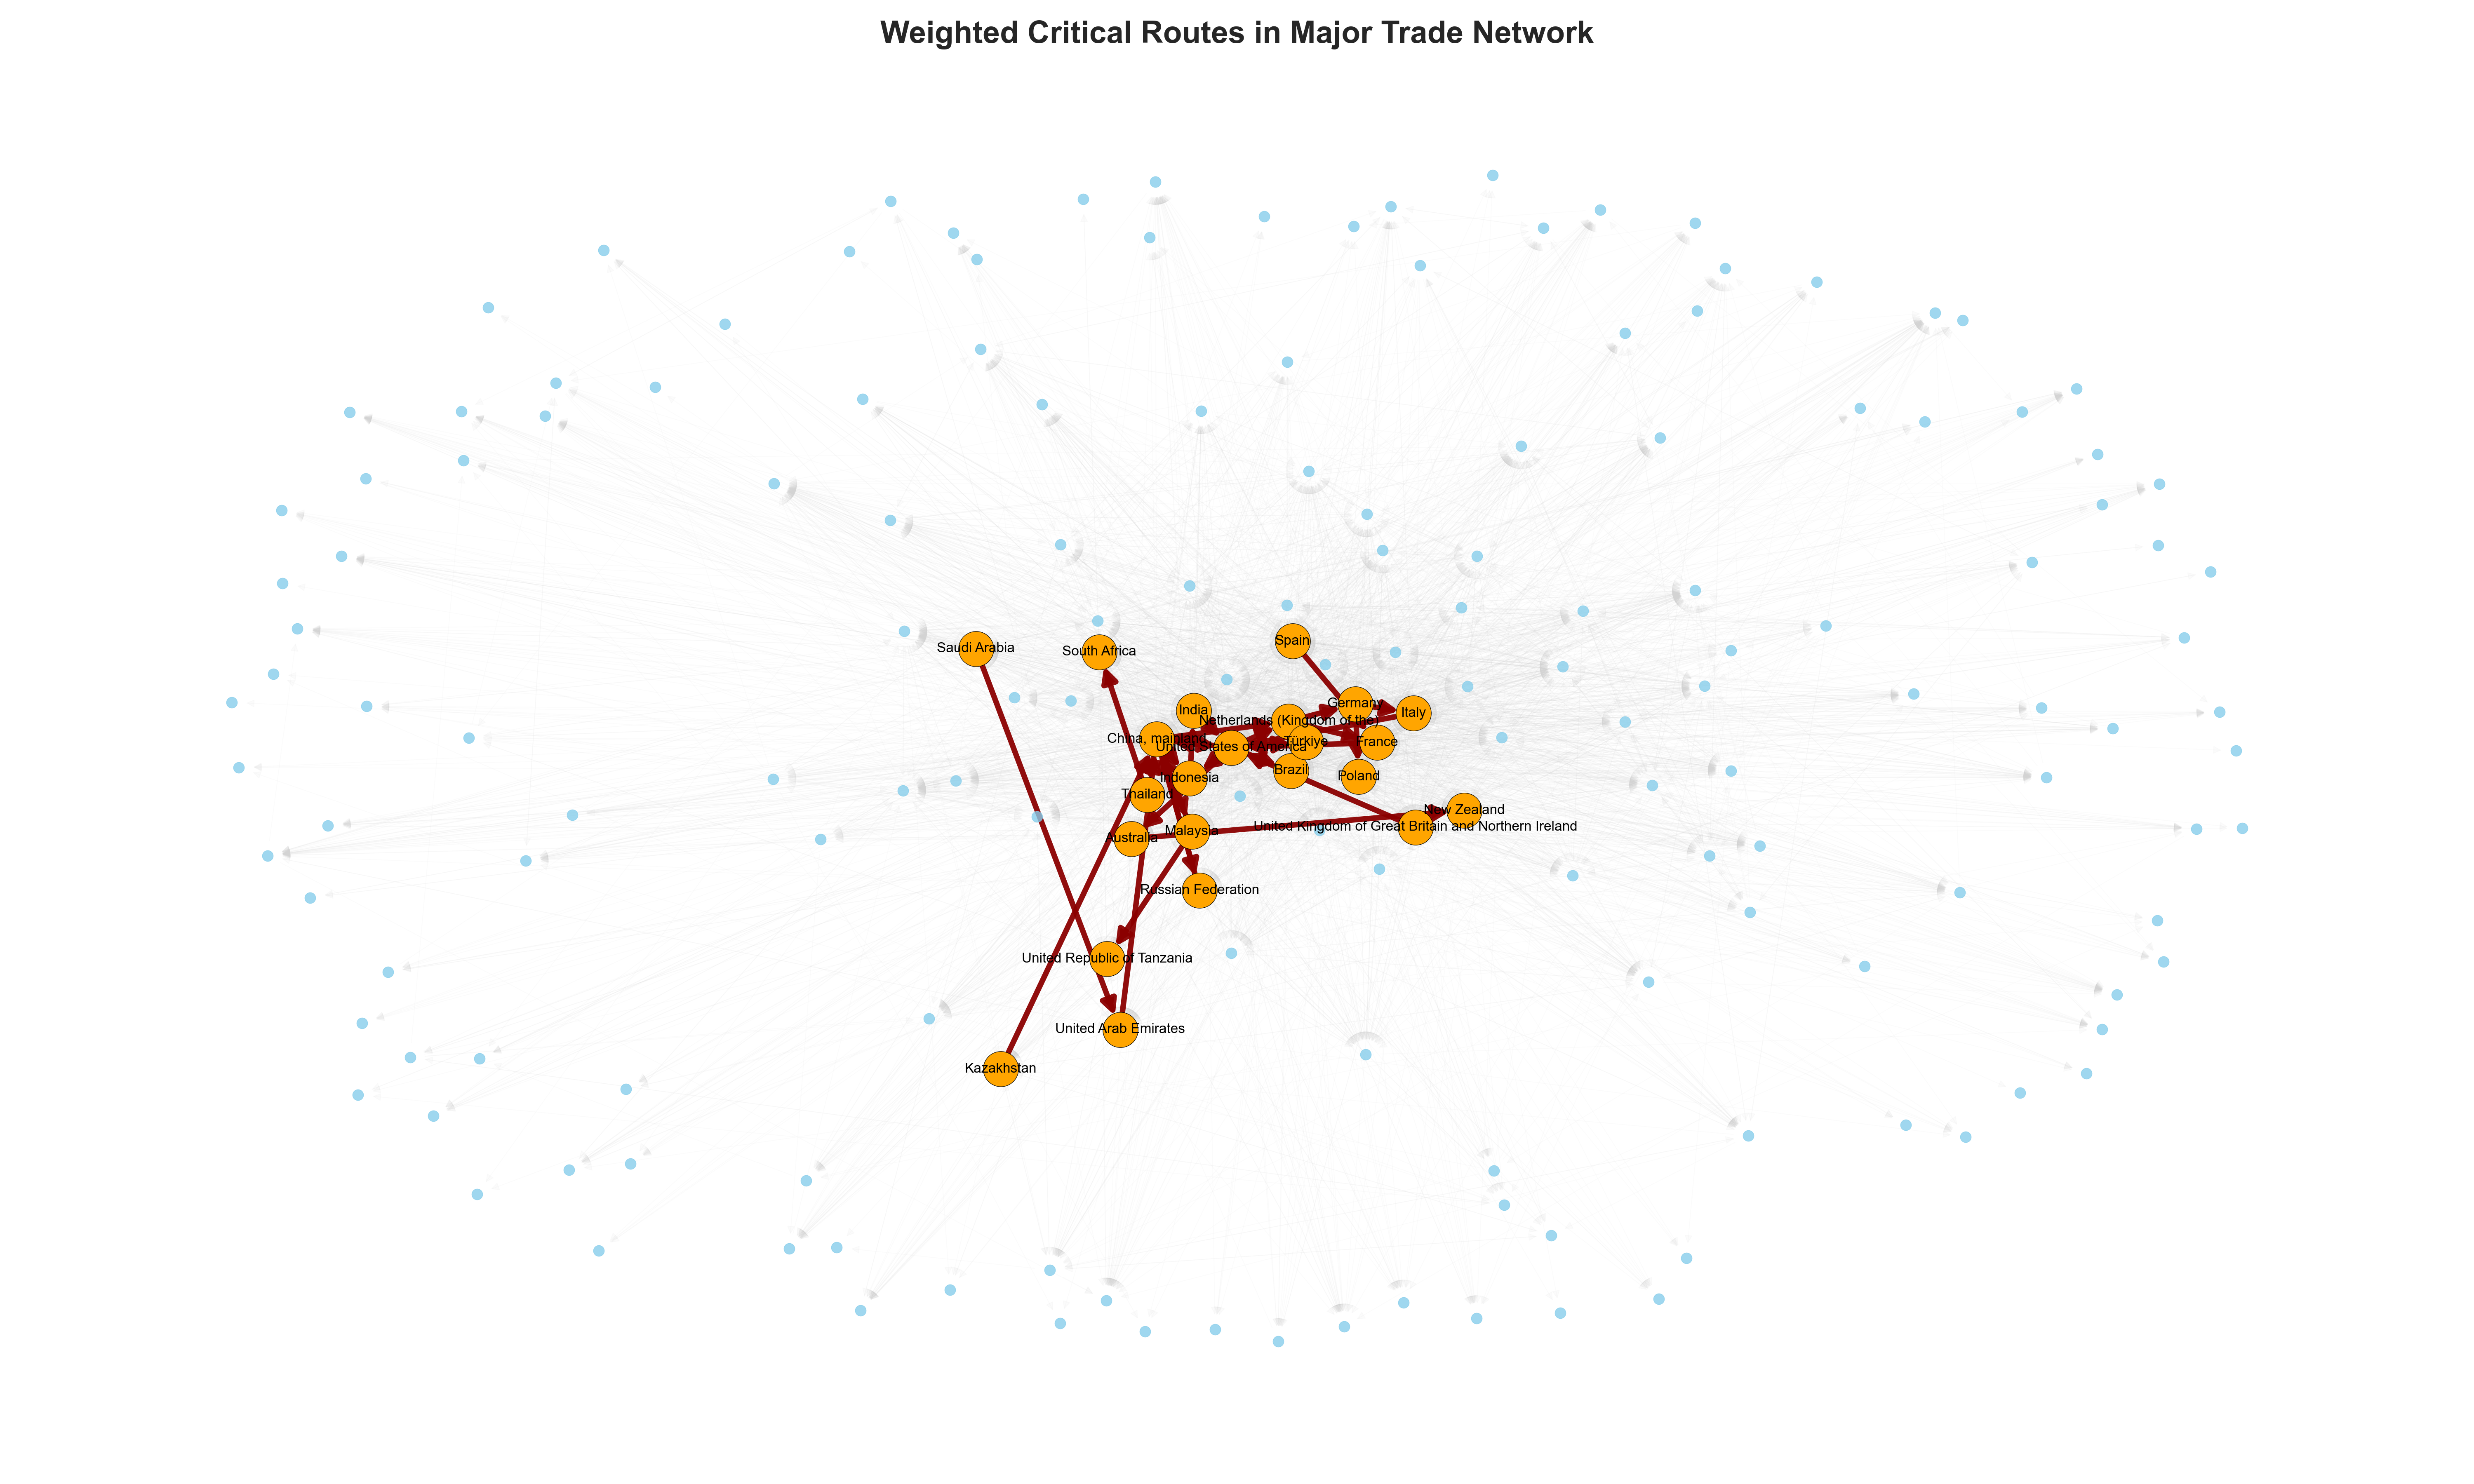
\includegraphics[width=\linewidth]{11b_weighted_highlighted_routes.png}
    \caption{Weighted critical routes overlay.}
  \end{subfigure}
  \caption{Location of critical corridors in the global network.}
  \label{fig:critical-overlays}
\end{figure}

\paragraph{Edge risk takeaways.}
\begin{itemize}
  \item Edge weights are highly concentrated: few corridors move a large share of value.
  \item Low-value routes can still be structurally important bridges.
  \item Resilience requires redundancy for both high-value and high-betweenness corridors.
\end{itemize}

\section{Critical Countries: Who Holds the System Together}
Country importance is assessed via volume (exports/imports), influence (PageRank), bridging (betweenness), and ``damage if removed'' under targeted attacks.

\subsection{Who feeds vs who depends}
\begin{figure}[H]
  \centering
  \begin{subfigure}[t]{0.49\linewidth}
    \centering
    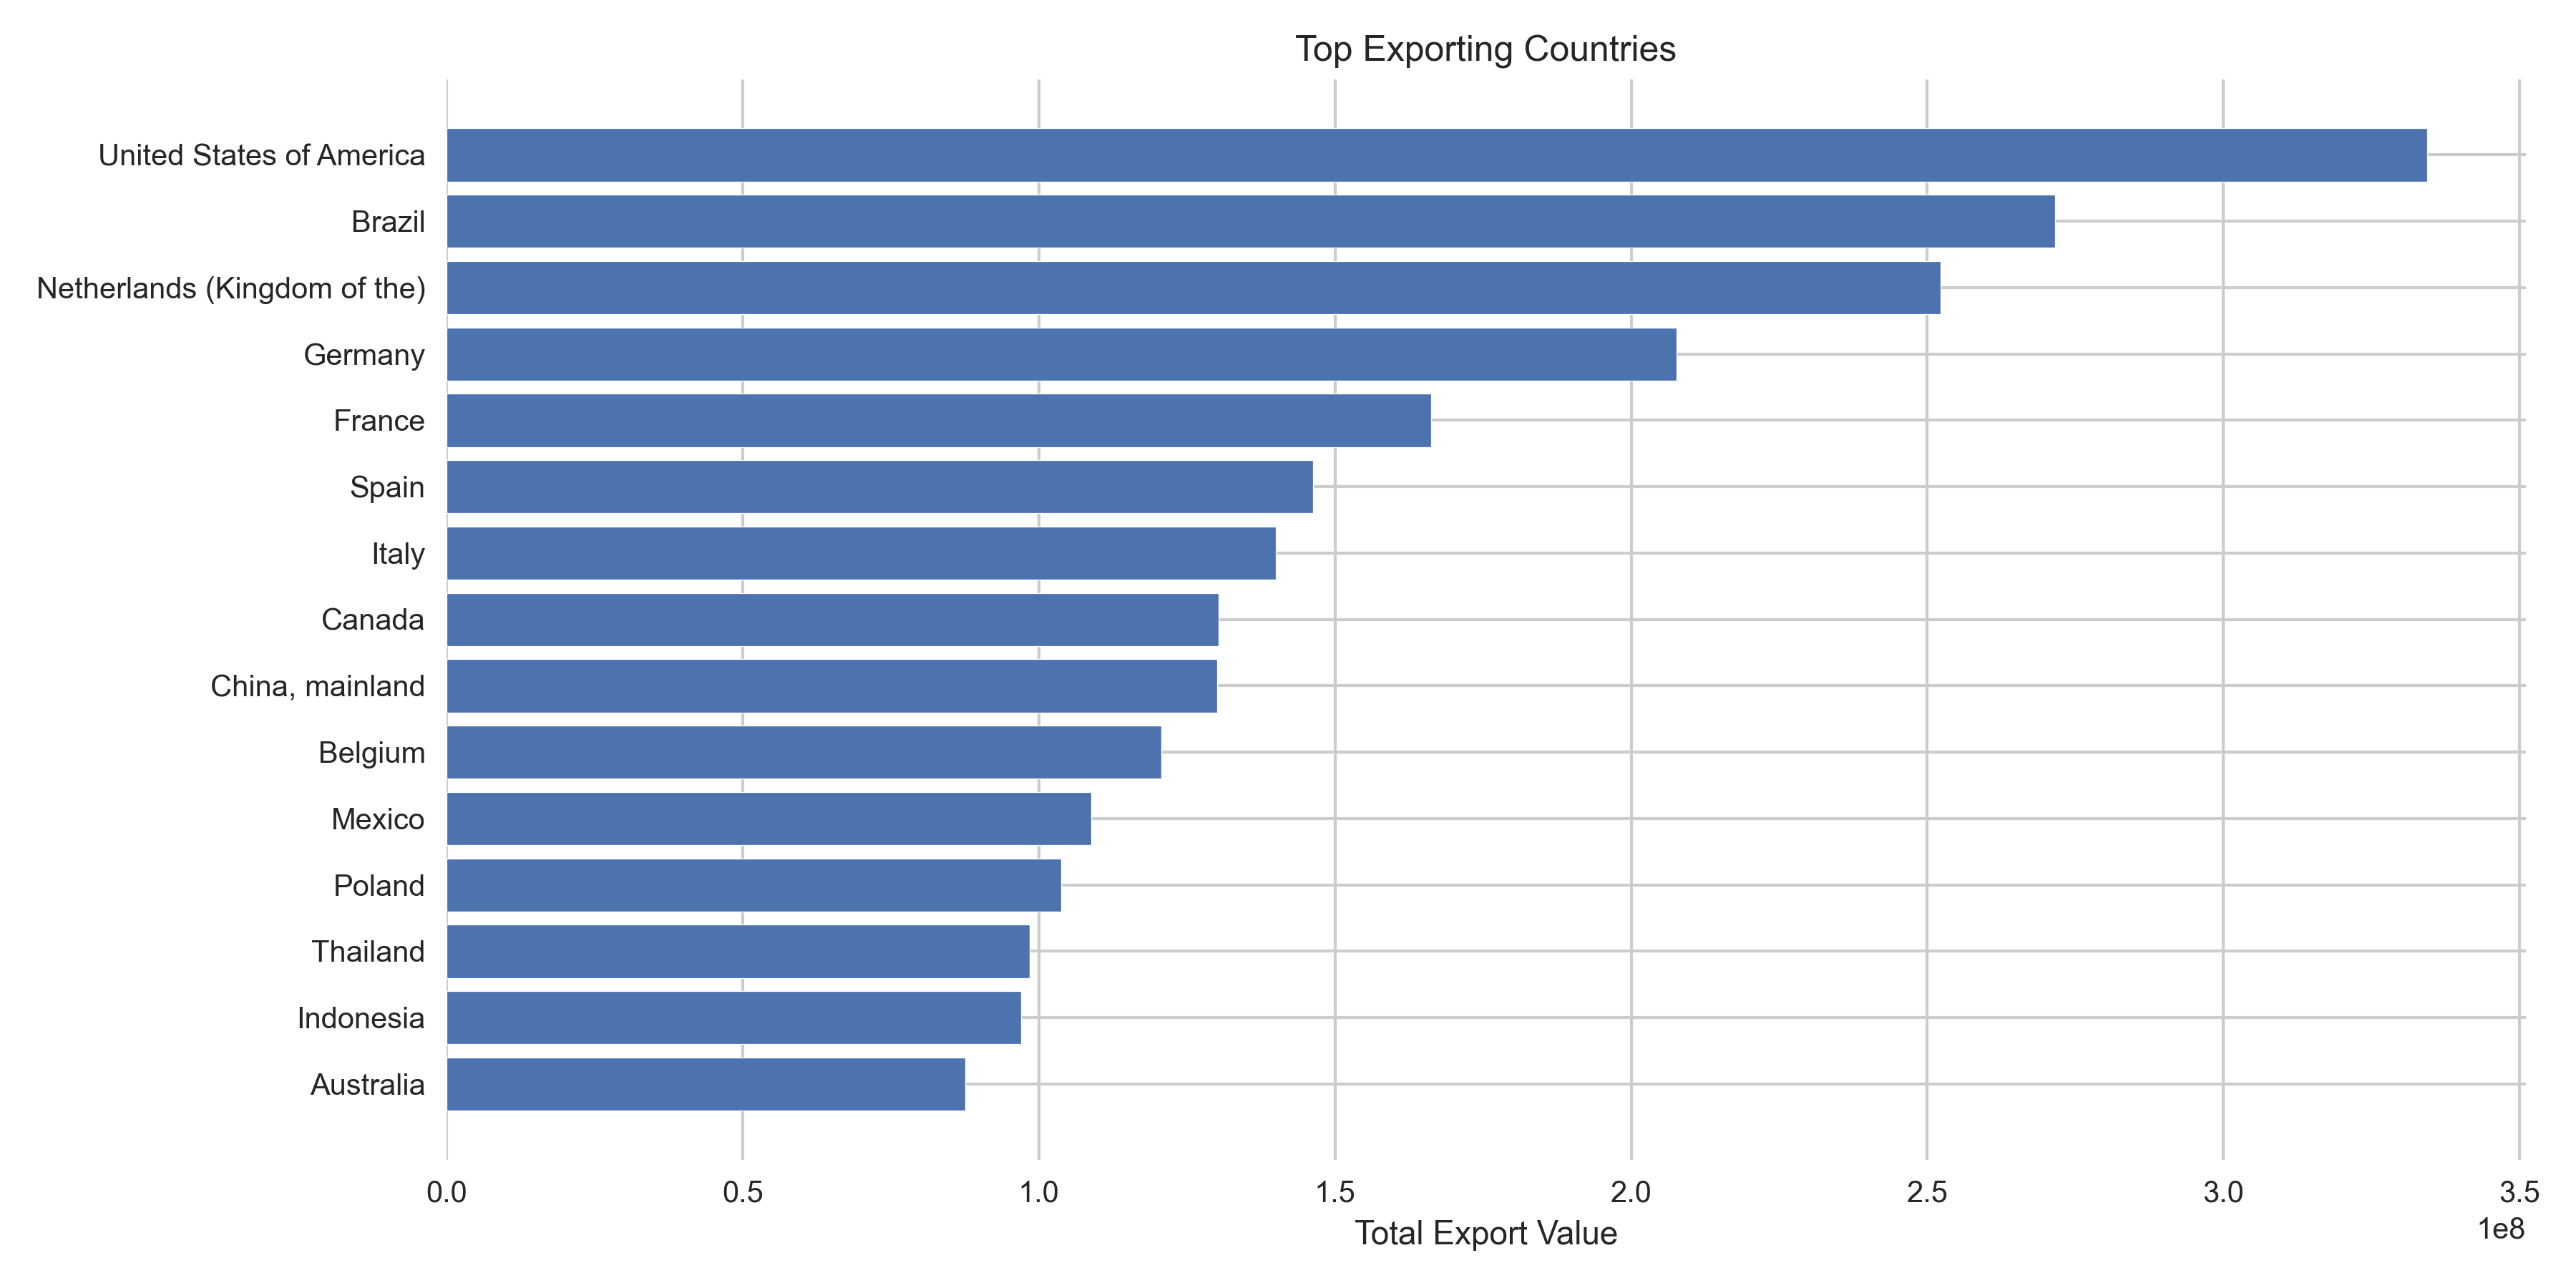
\includegraphics[width=\linewidth]{05_top_exporters.png}
    \caption{Top exporters by outbound trade value.}
  \end{subfigure}
  \hfill
  \begin{subfigure}[t]{0.49\linewidth}
    \centering
    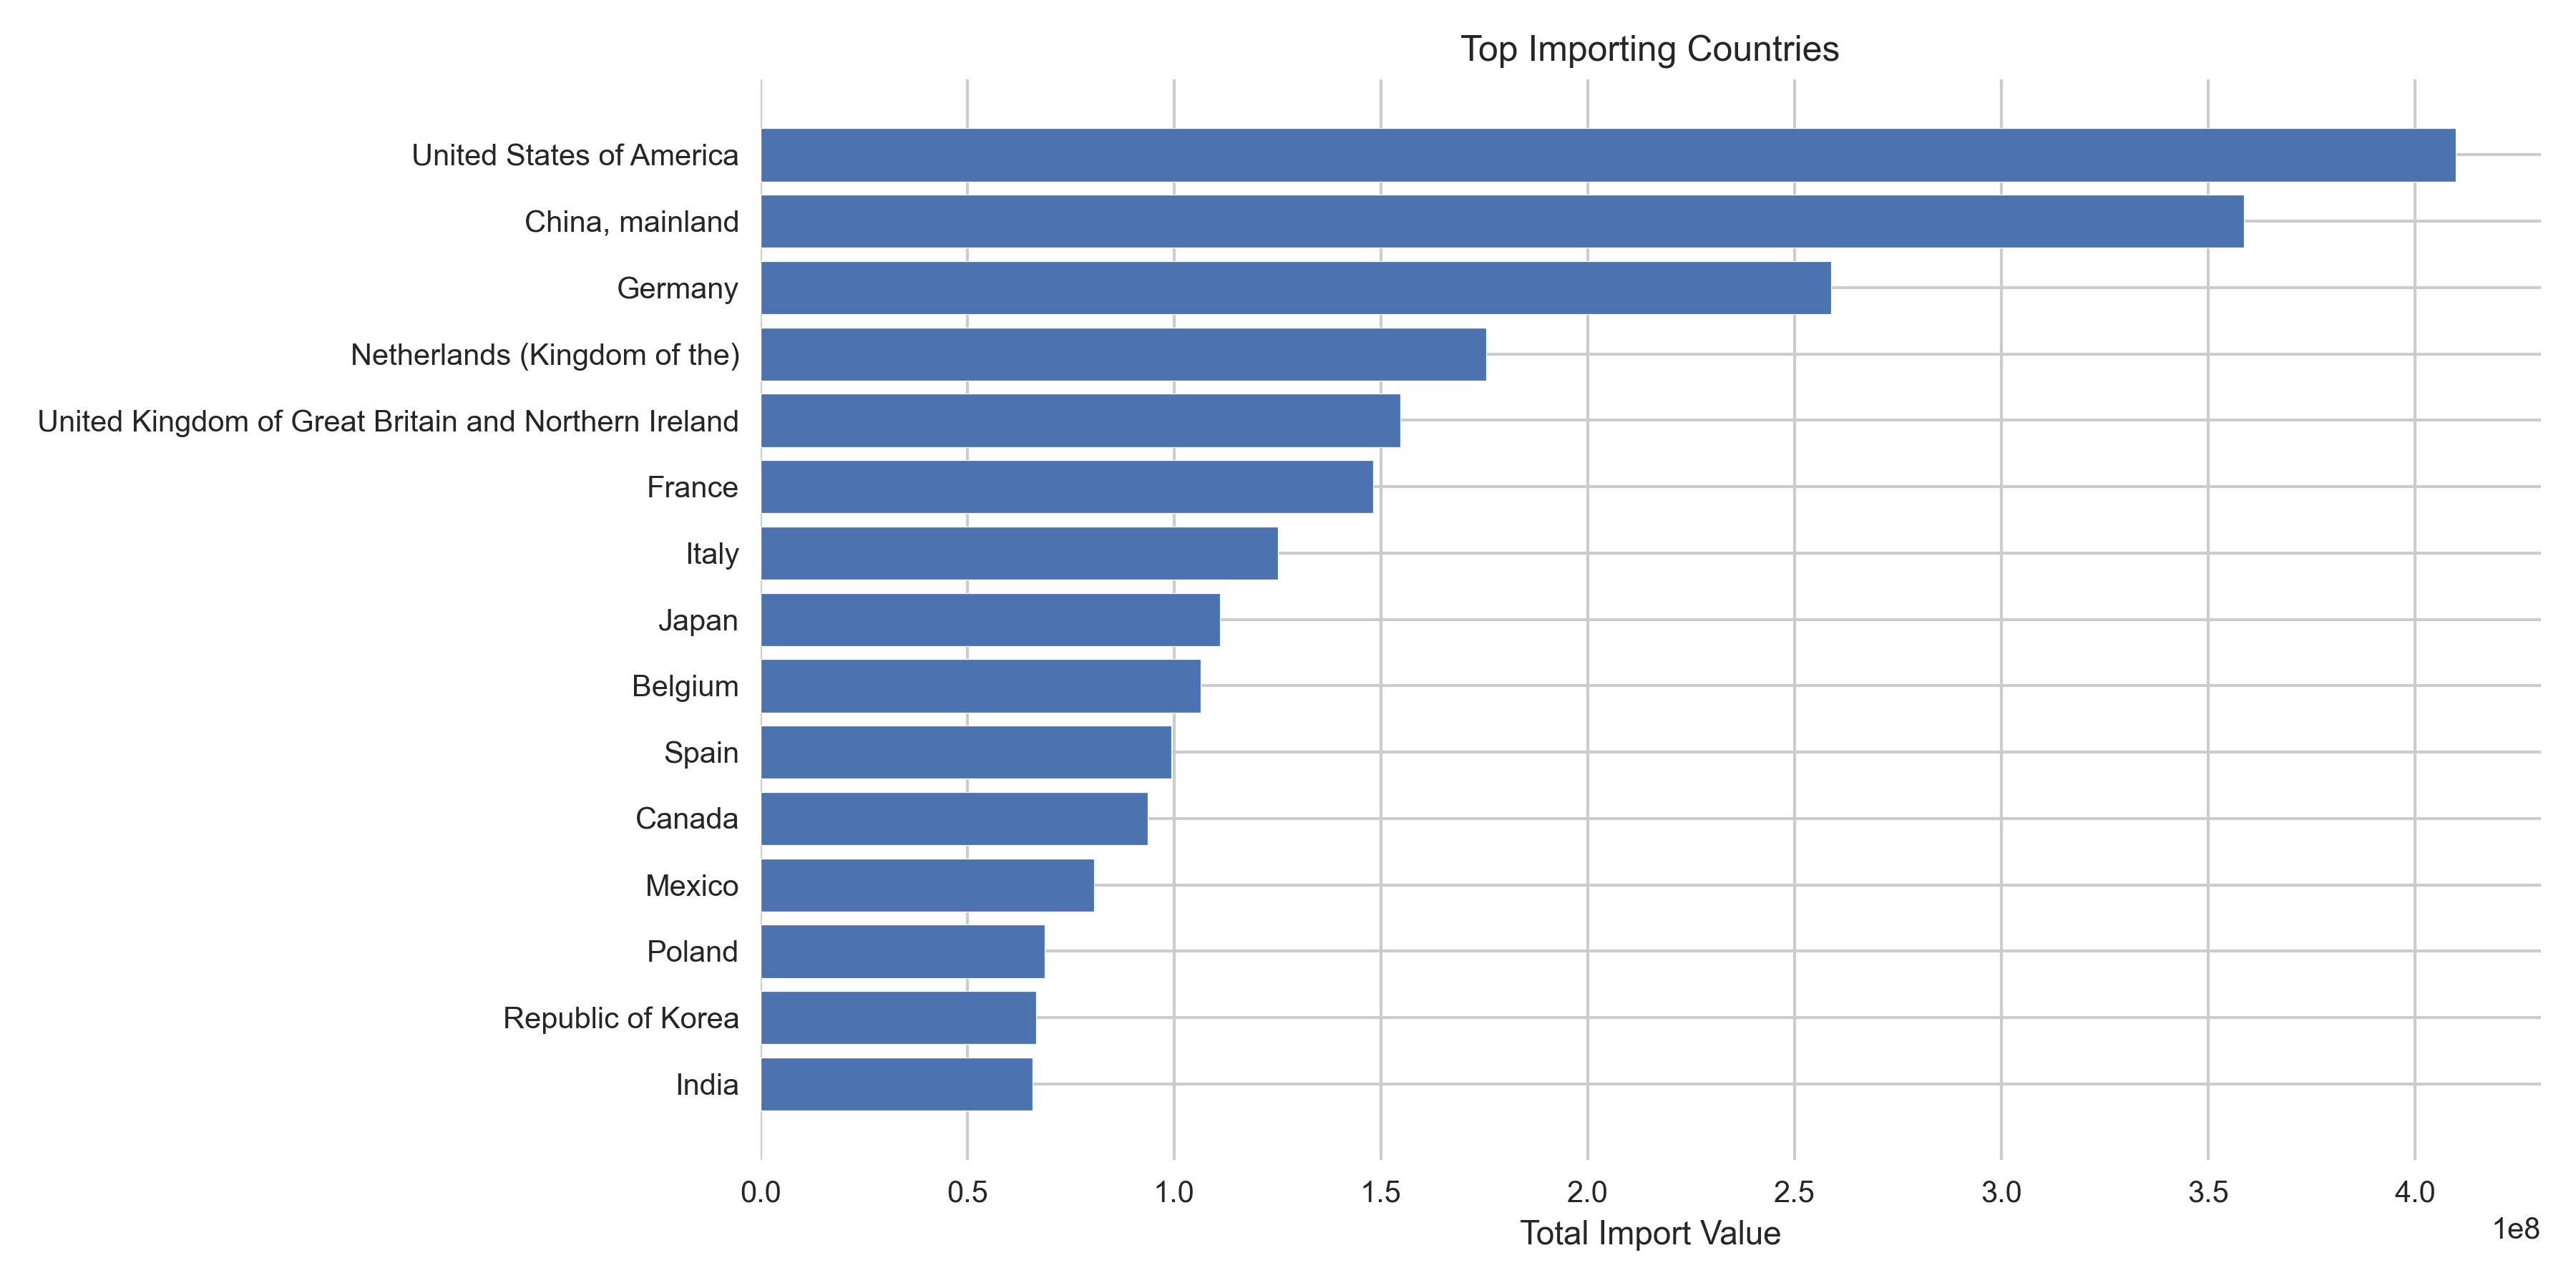
\includegraphics[width=\linewidth]{06_top_importers.png}
    \caption{Top importers by inbound trade value.}
  \end{subfigure}
  \caption{Major exporting and importing countries in the network.}
  \label{fig:export-import}
\end{figure}

\begin{figure}[H]
  \centering
  \begin{subfigure}[t]{0.49\linewidth}
    \centering
    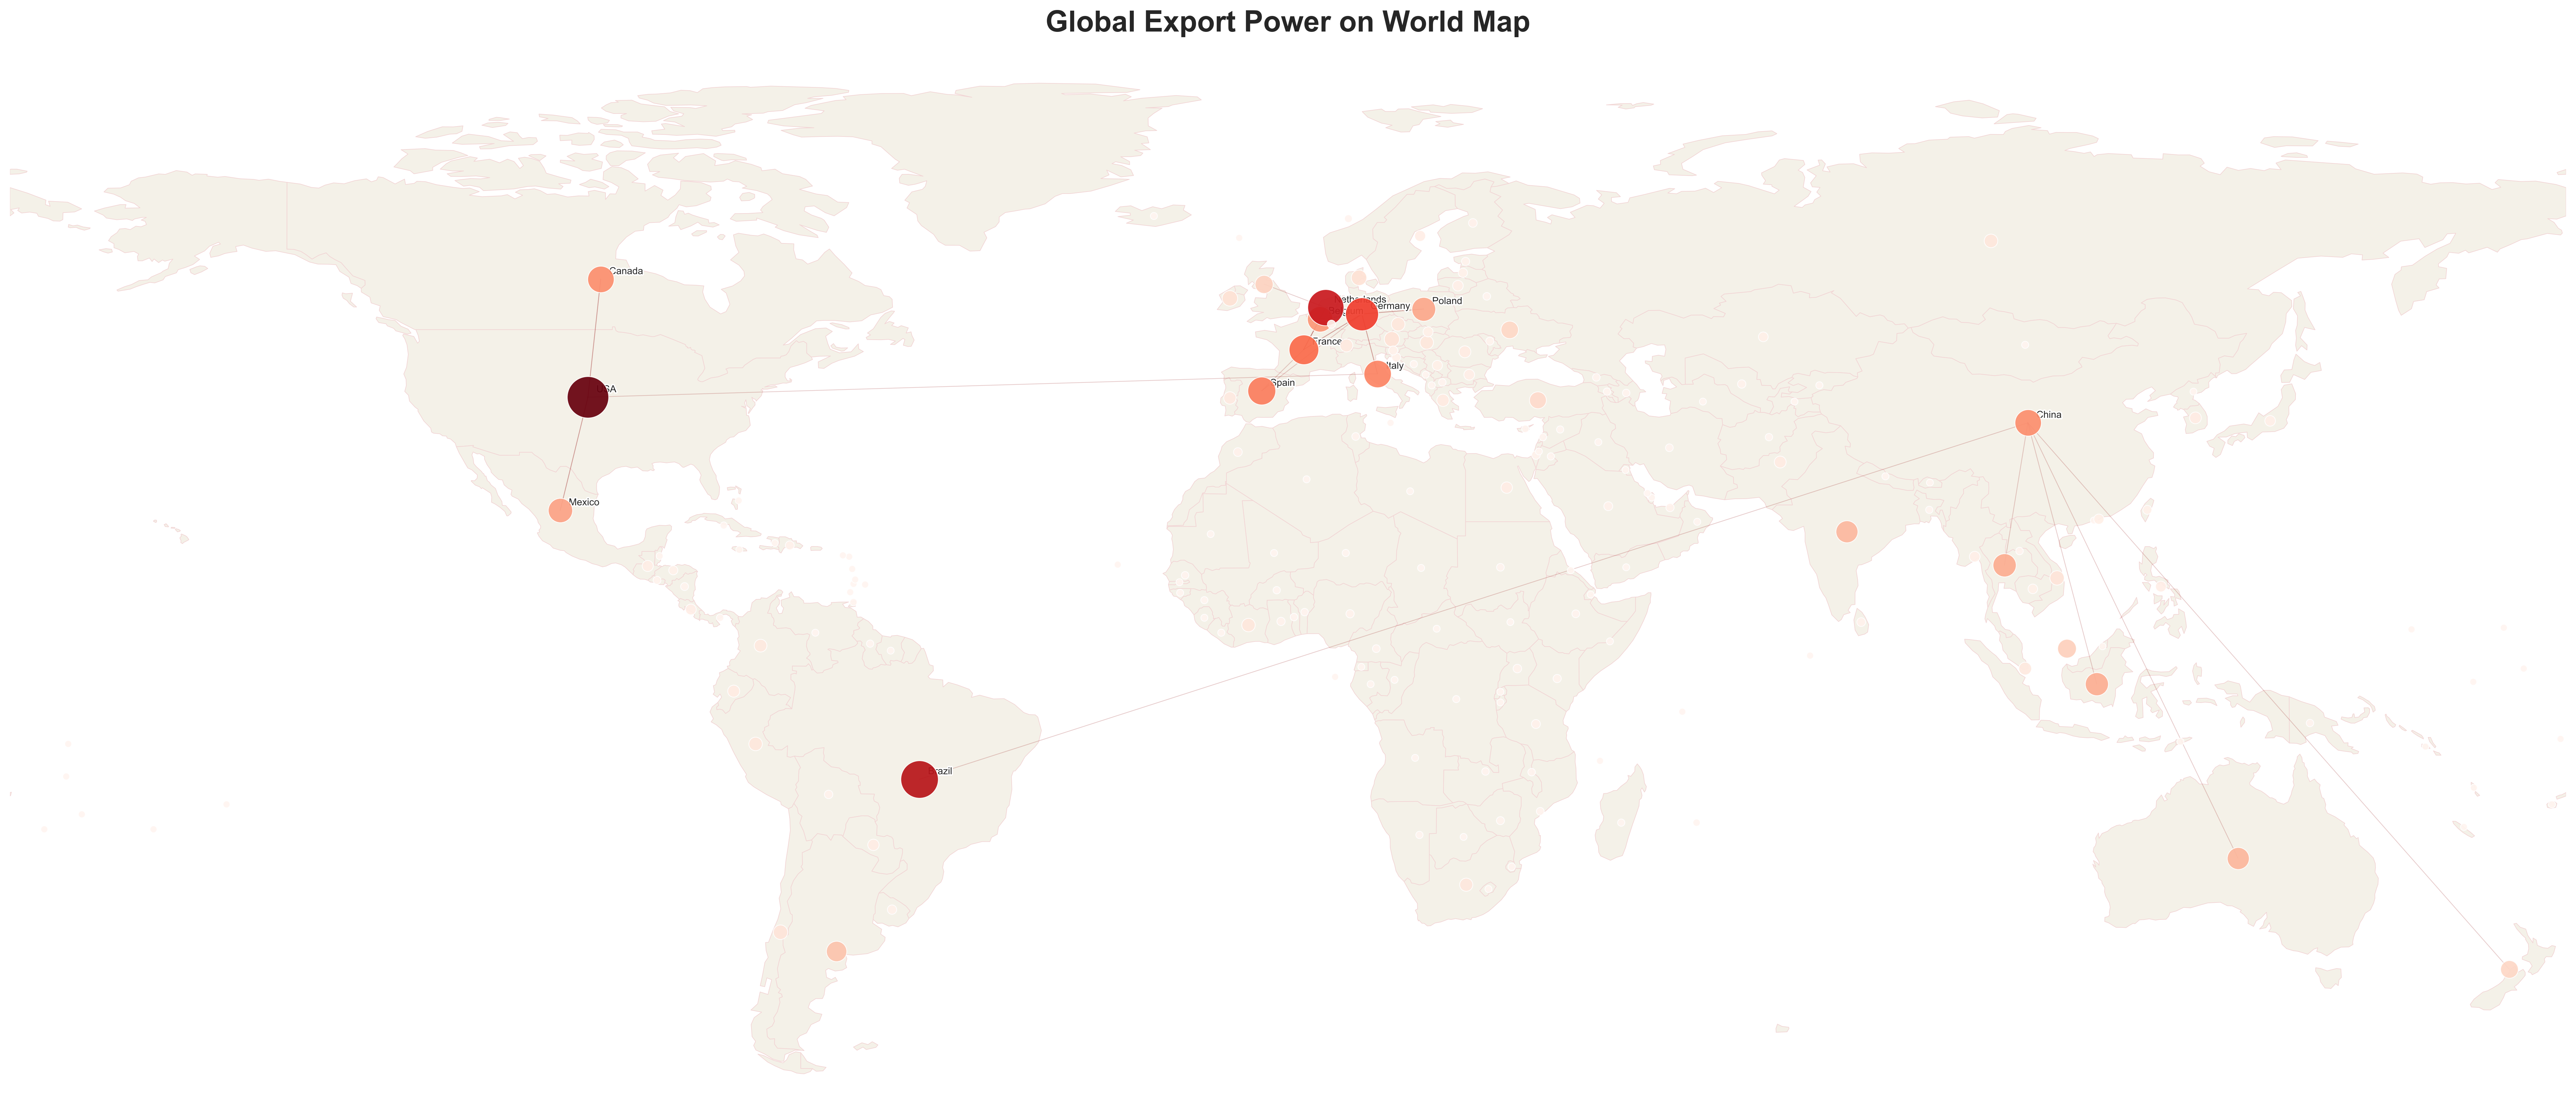
\includegraphics[width=\linewidth]{37_world_map_exporters.png}
    \caption{Export power (map).}
  \end{subfigure}
  \hfill
  \begin{subfigure}[t]{0.49\linewidth}
    \centering
    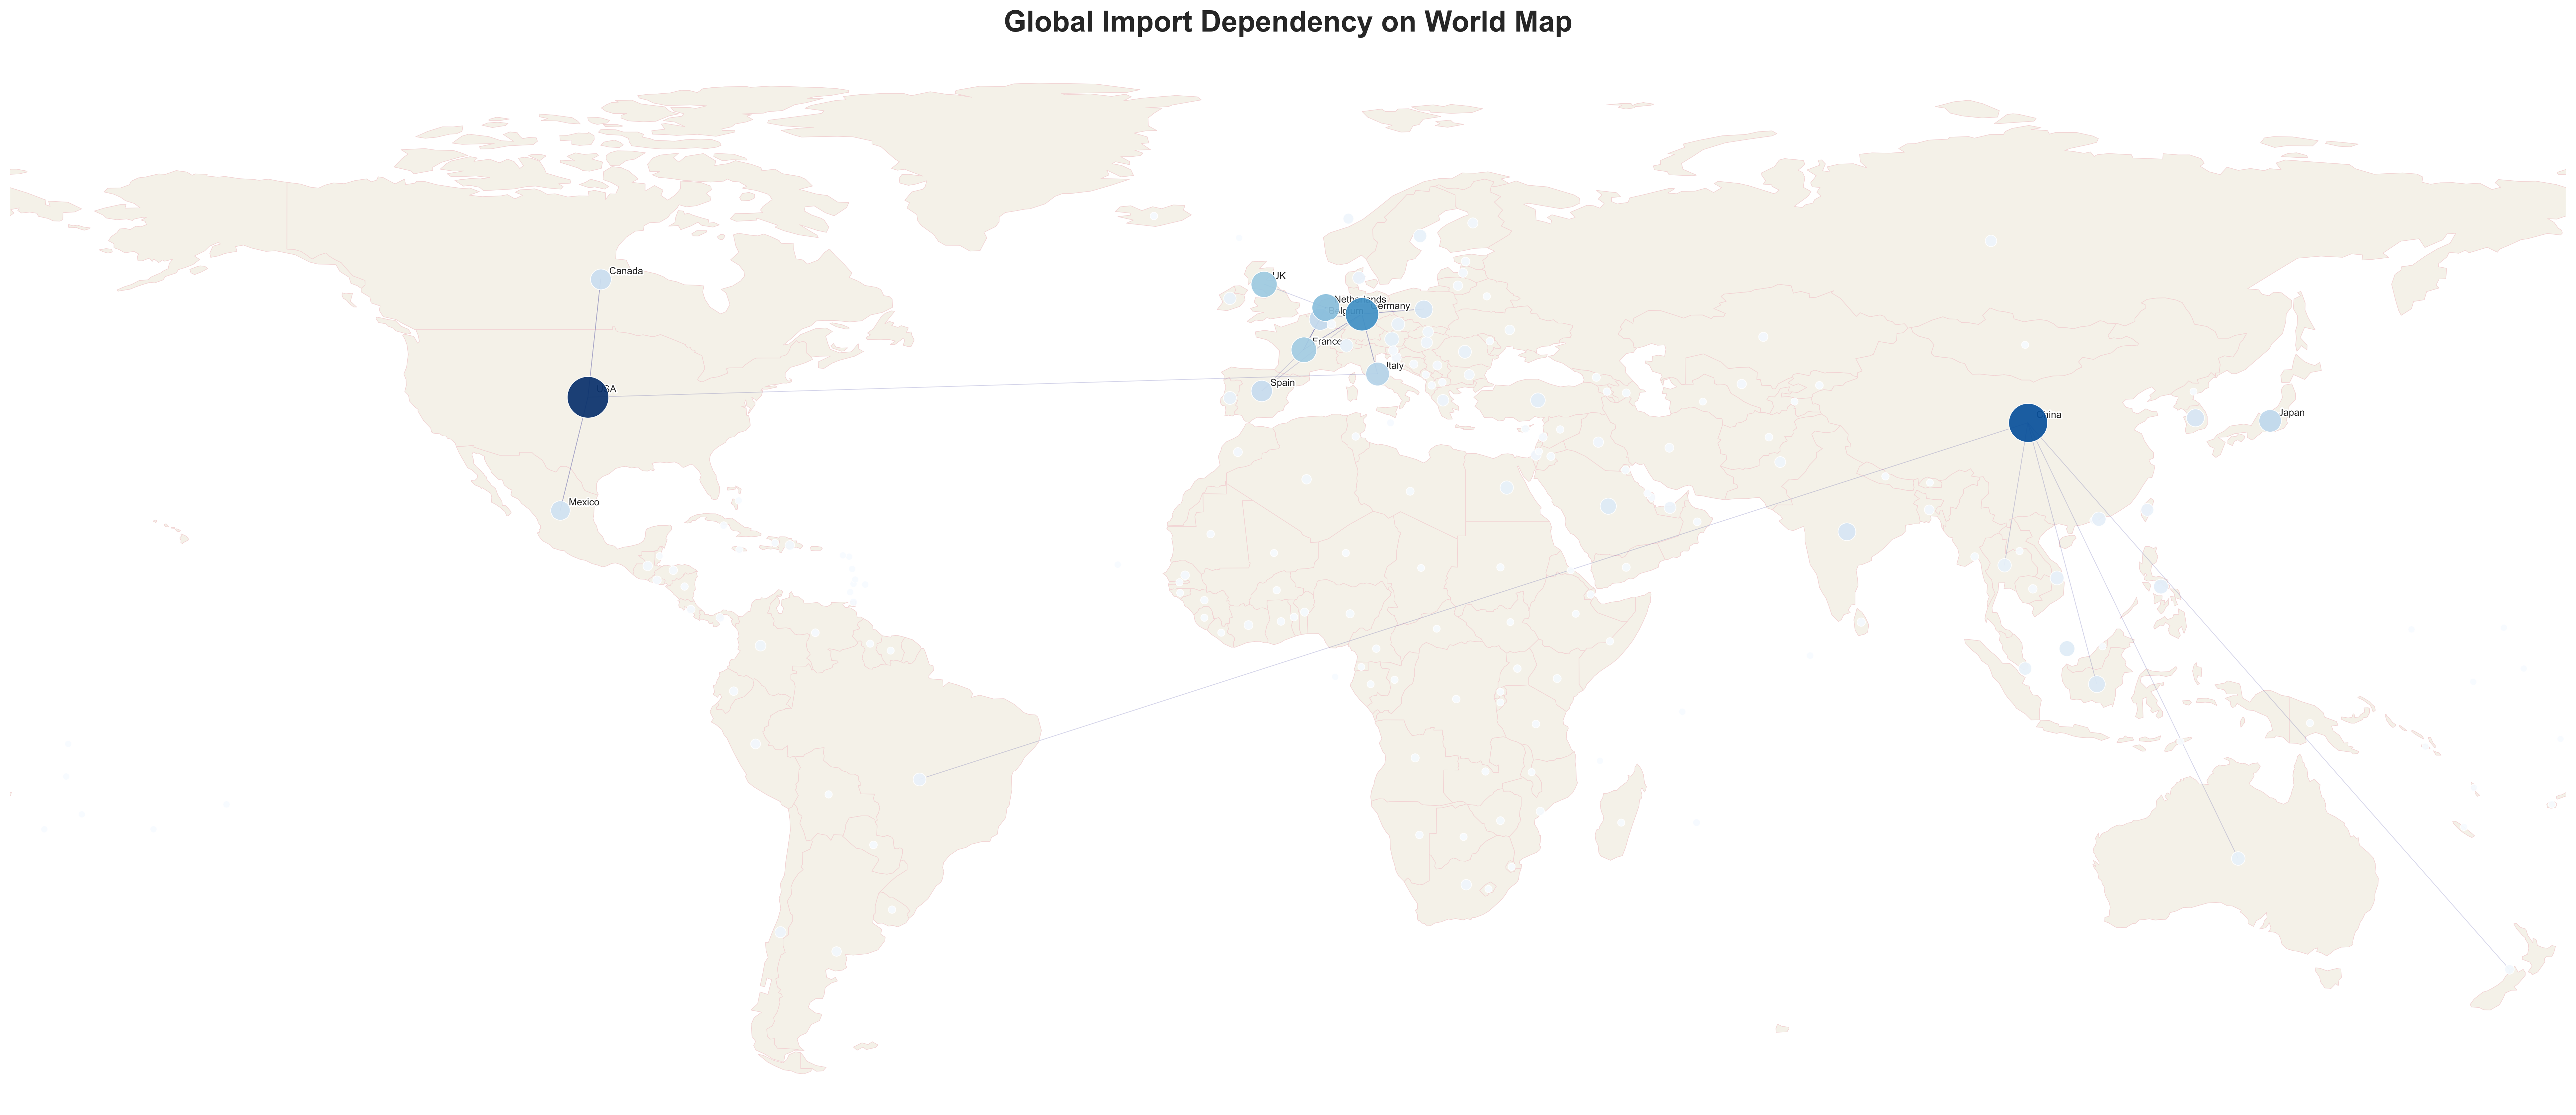
\includegraphics[width=\linewidth]{38_world_map_importers.png}
    \caption{Import dependency (map).}
  \end{subfigure}
  \caption{Geographic structure of export concentration and import reliance.}
  \label{fig:export-import-maps}
\end{figure}

\subsection{Influence and bridging}
\begin{figure}[H]
  \centering
  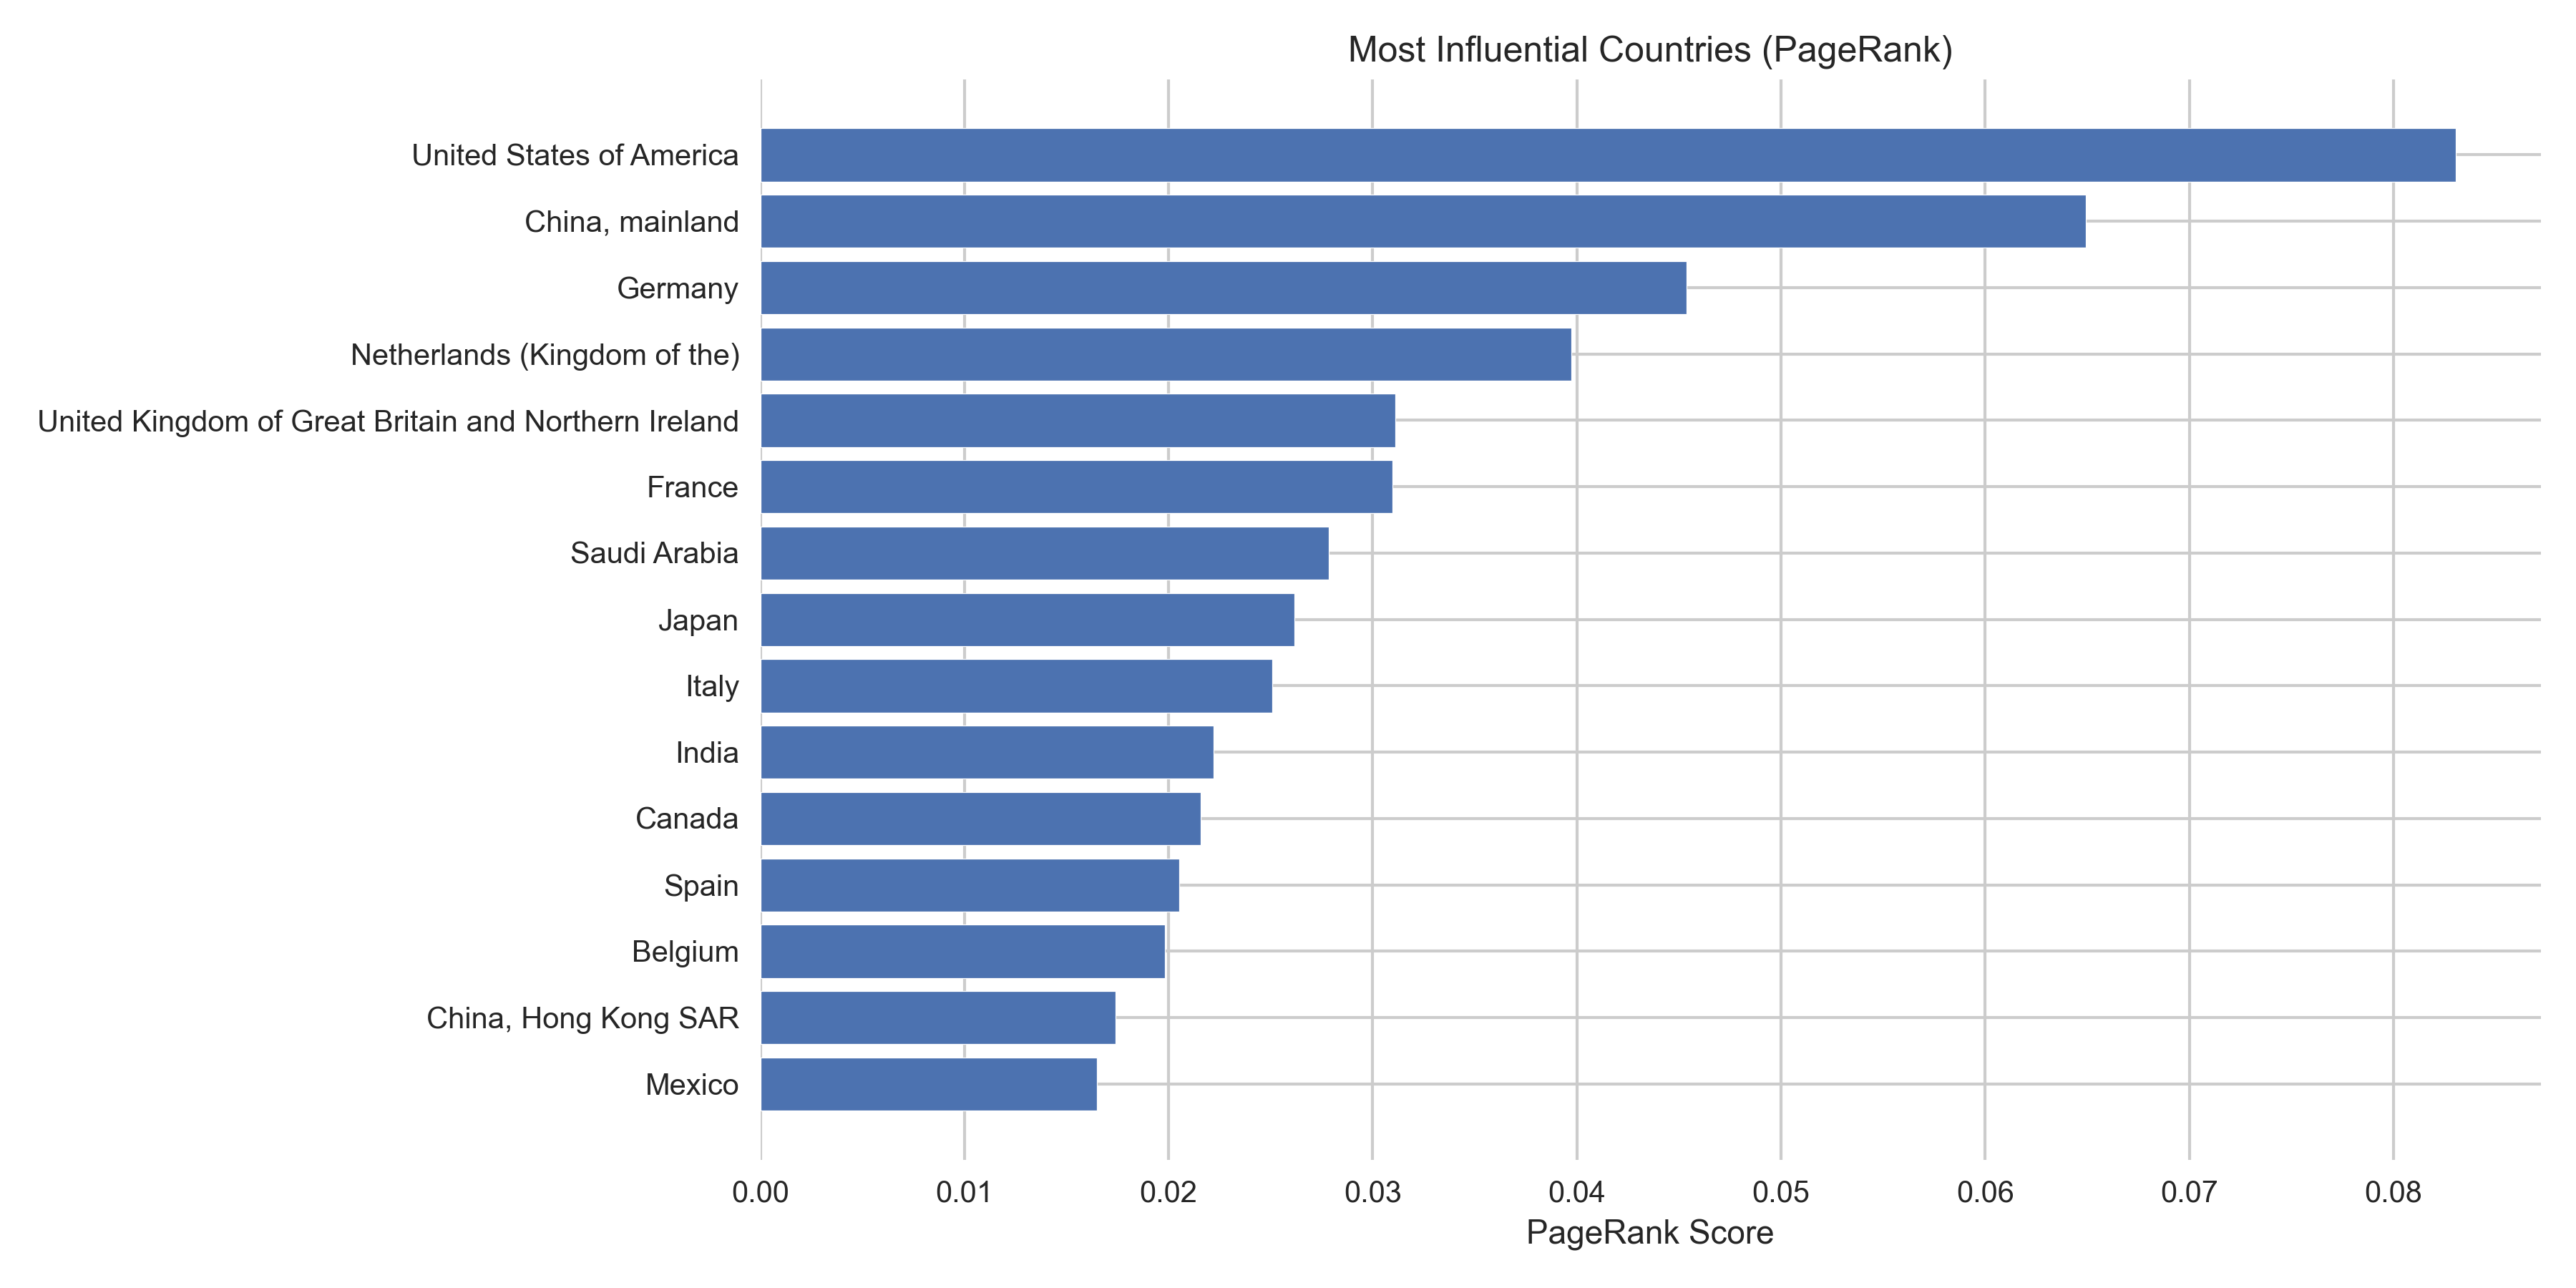
\includegraphics[width=0.92\linewidth]{07_top_pagerank.png}
  \caption{PageRank-based influence: importance depends on position in the flow topology, not only volume.}
  \label{fig:pagerank}
\end{figure}

\begin{figure}[H]
  \centering
  \begin{subfigure}[t]{0.49\linewidth}
    \centering
    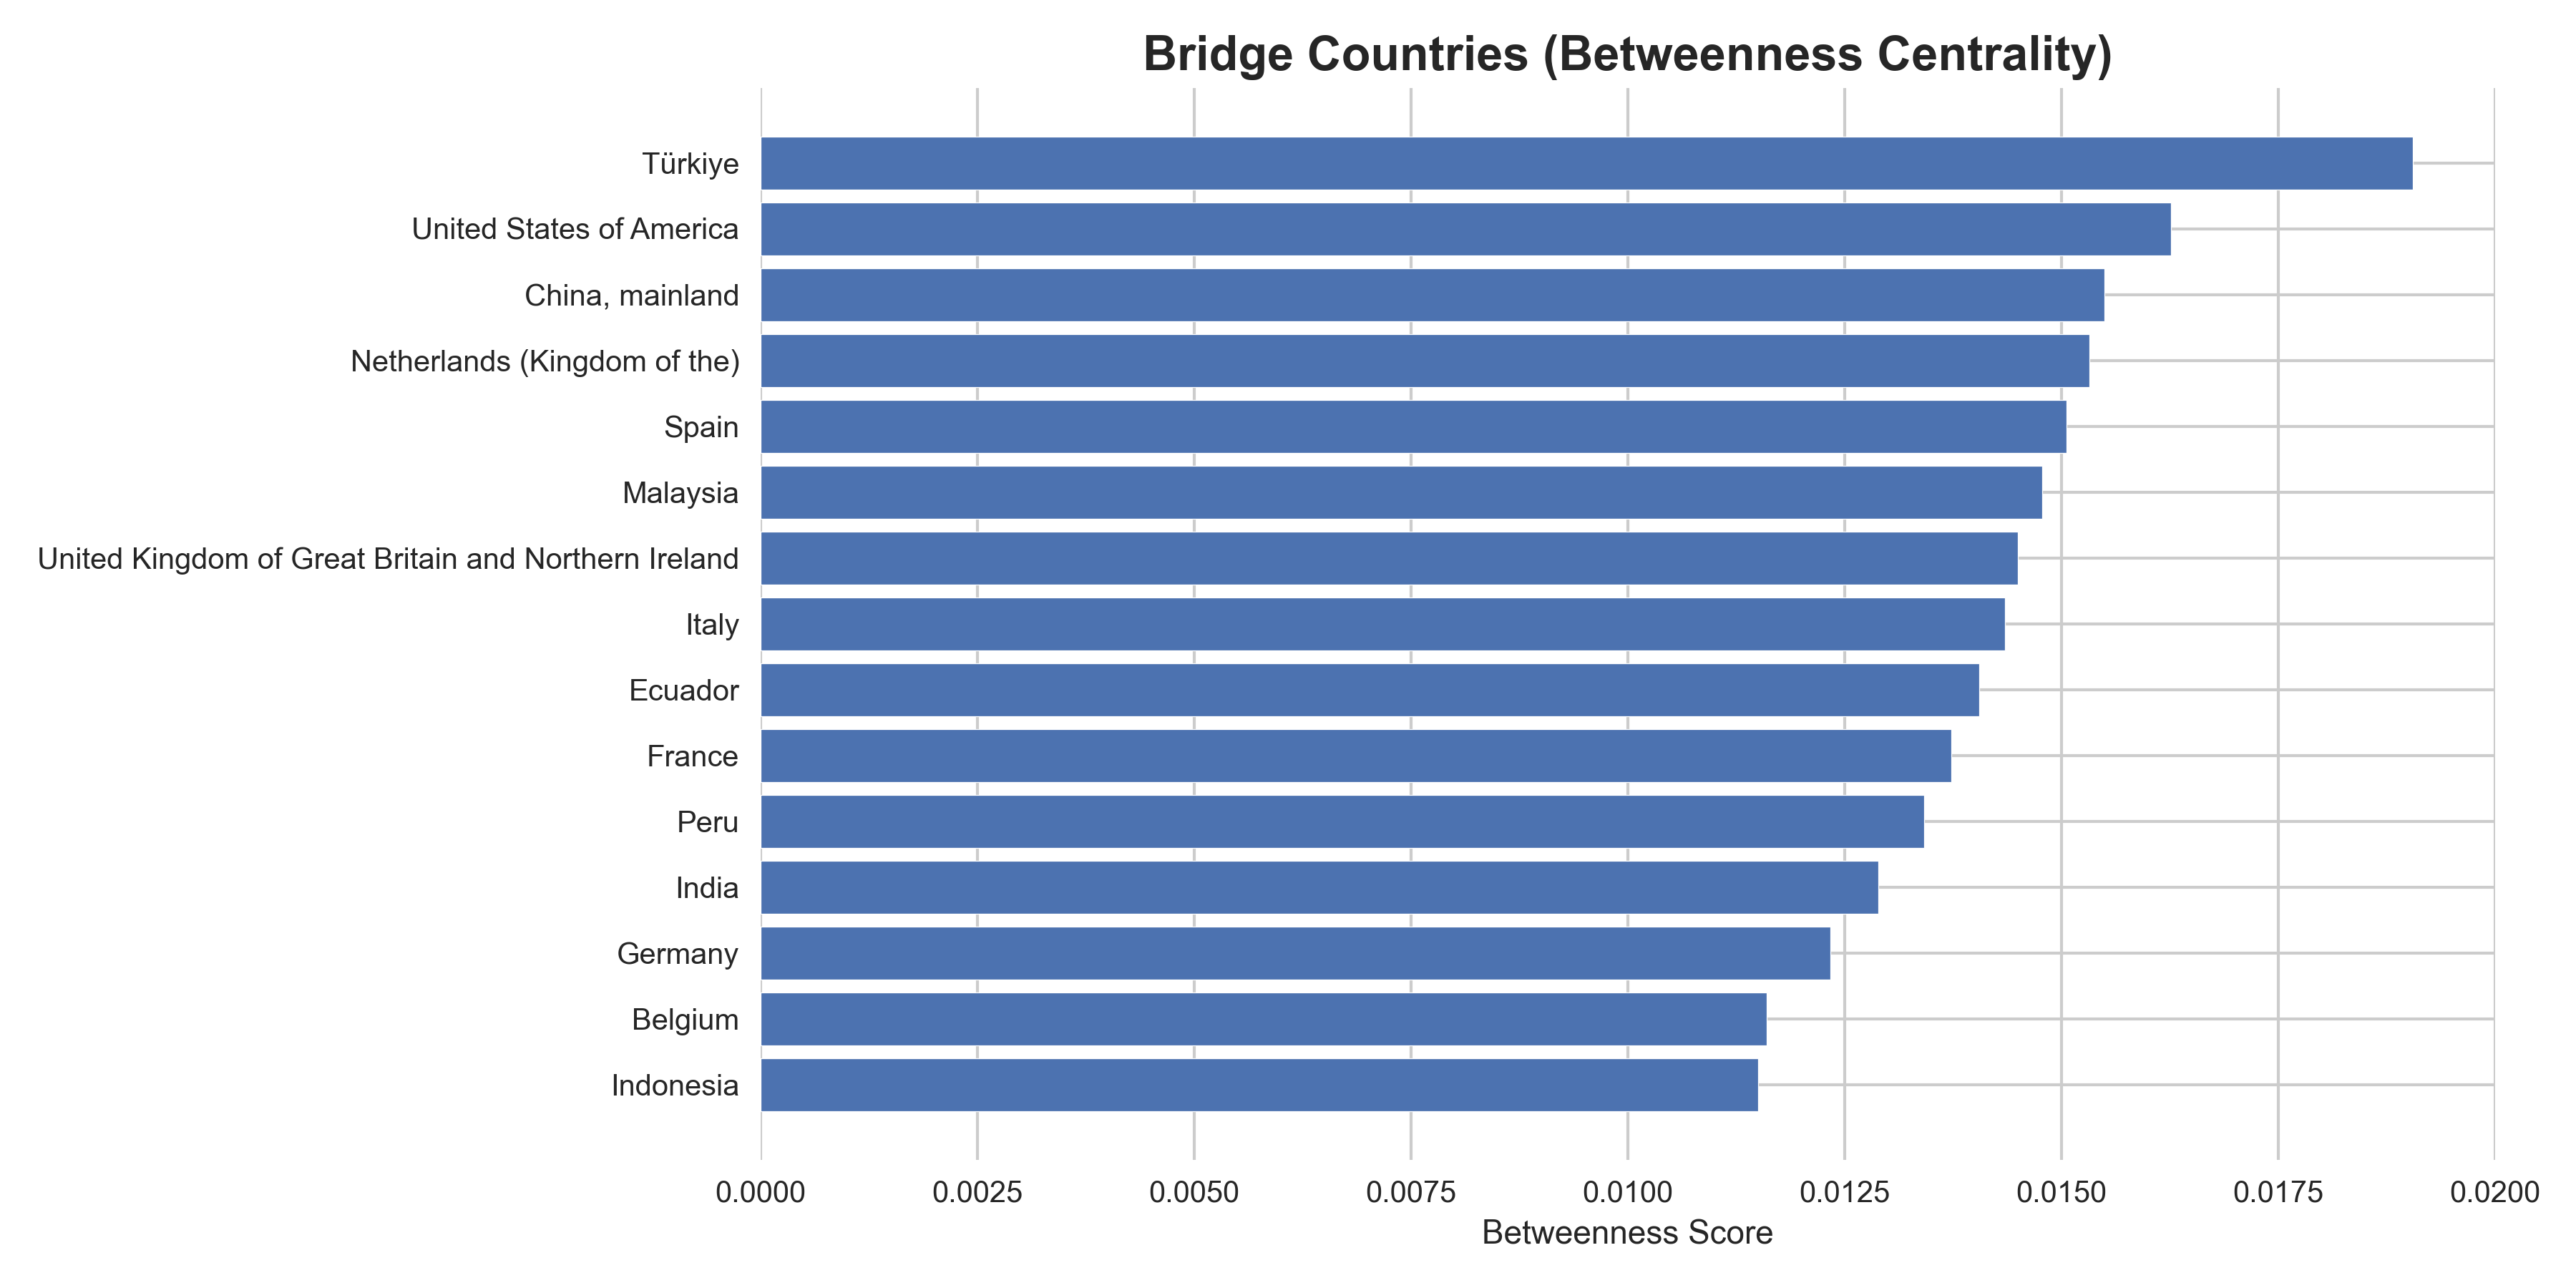
\includegraphics[width=\linewidth]{08_bridge_countries.png}
    \caption{Structural bridge countries (betweenness).}
  \end{subfigure}
  \hfill
  \begin{subfigure}[t]{0.49\linewidth}
    \centering
    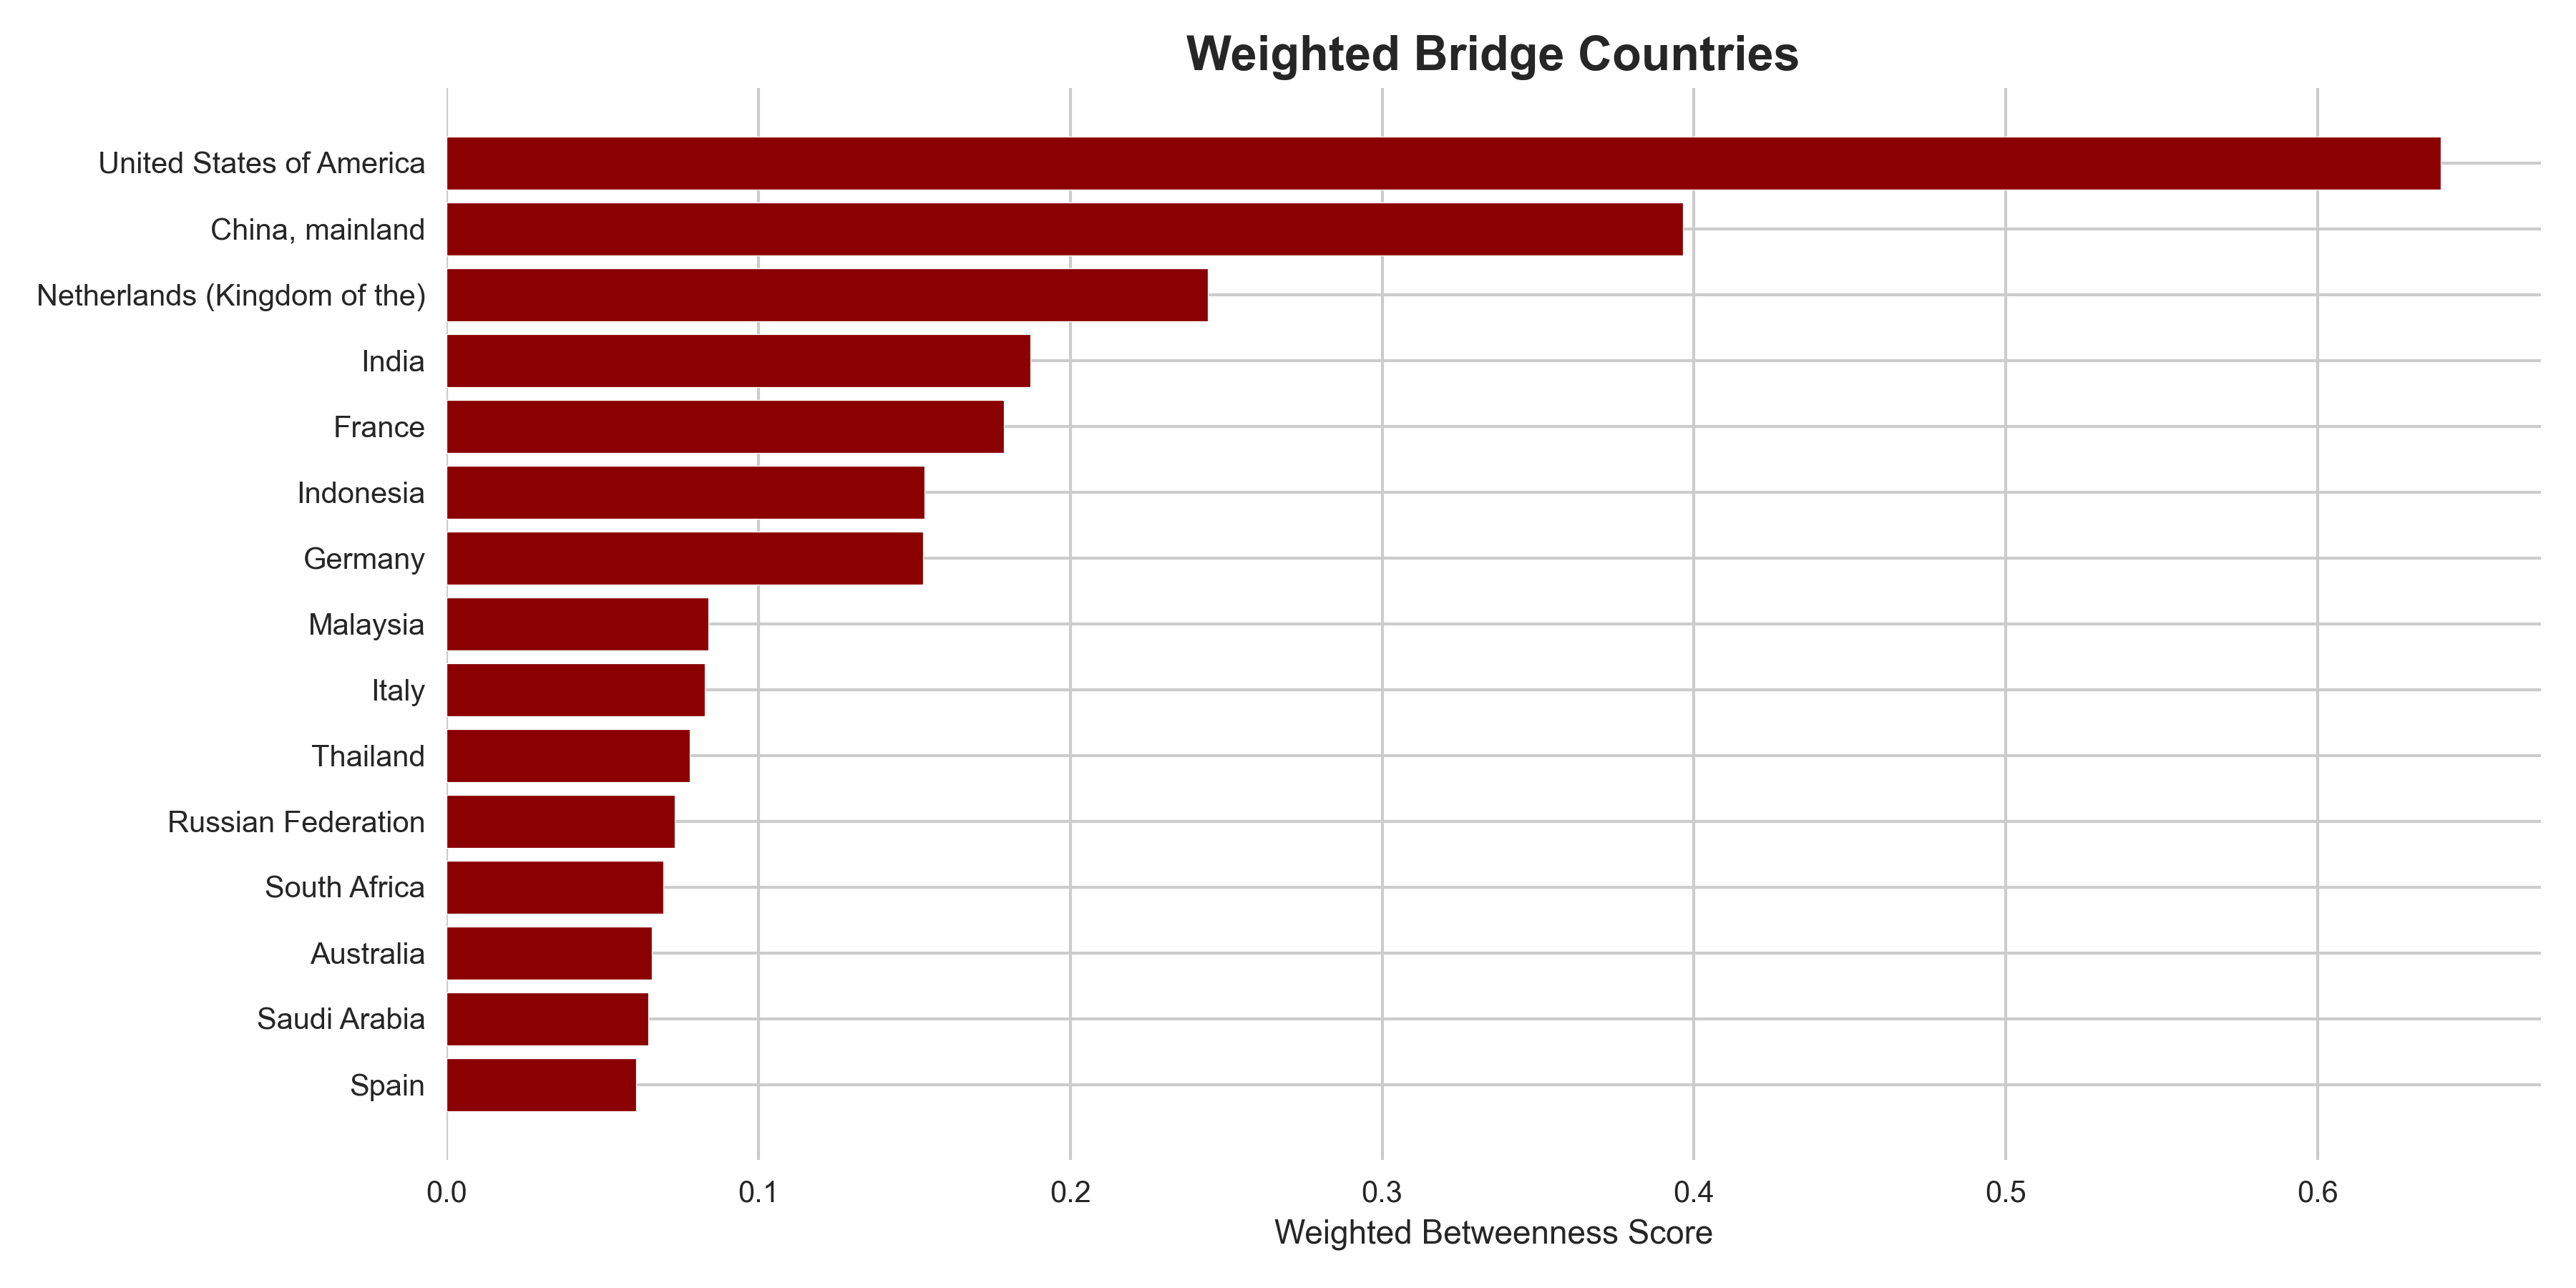
\includegraphics[width=\linewidth]{08b_weighted_bridge_countries.png}
    \caption{Weighted bridge countries (flow betweenness).}
  \end{subfigure}
  \caption{Bridging roles under structural vs weighted path definitions.}
  \label{fig:bridges}
\end{figure}

\subsection{Which removals cause the most damage?}
\begin{figure}[H]
  \centering
  \begin{subfigure}[t]{0.49\linewidth}
    \centering
    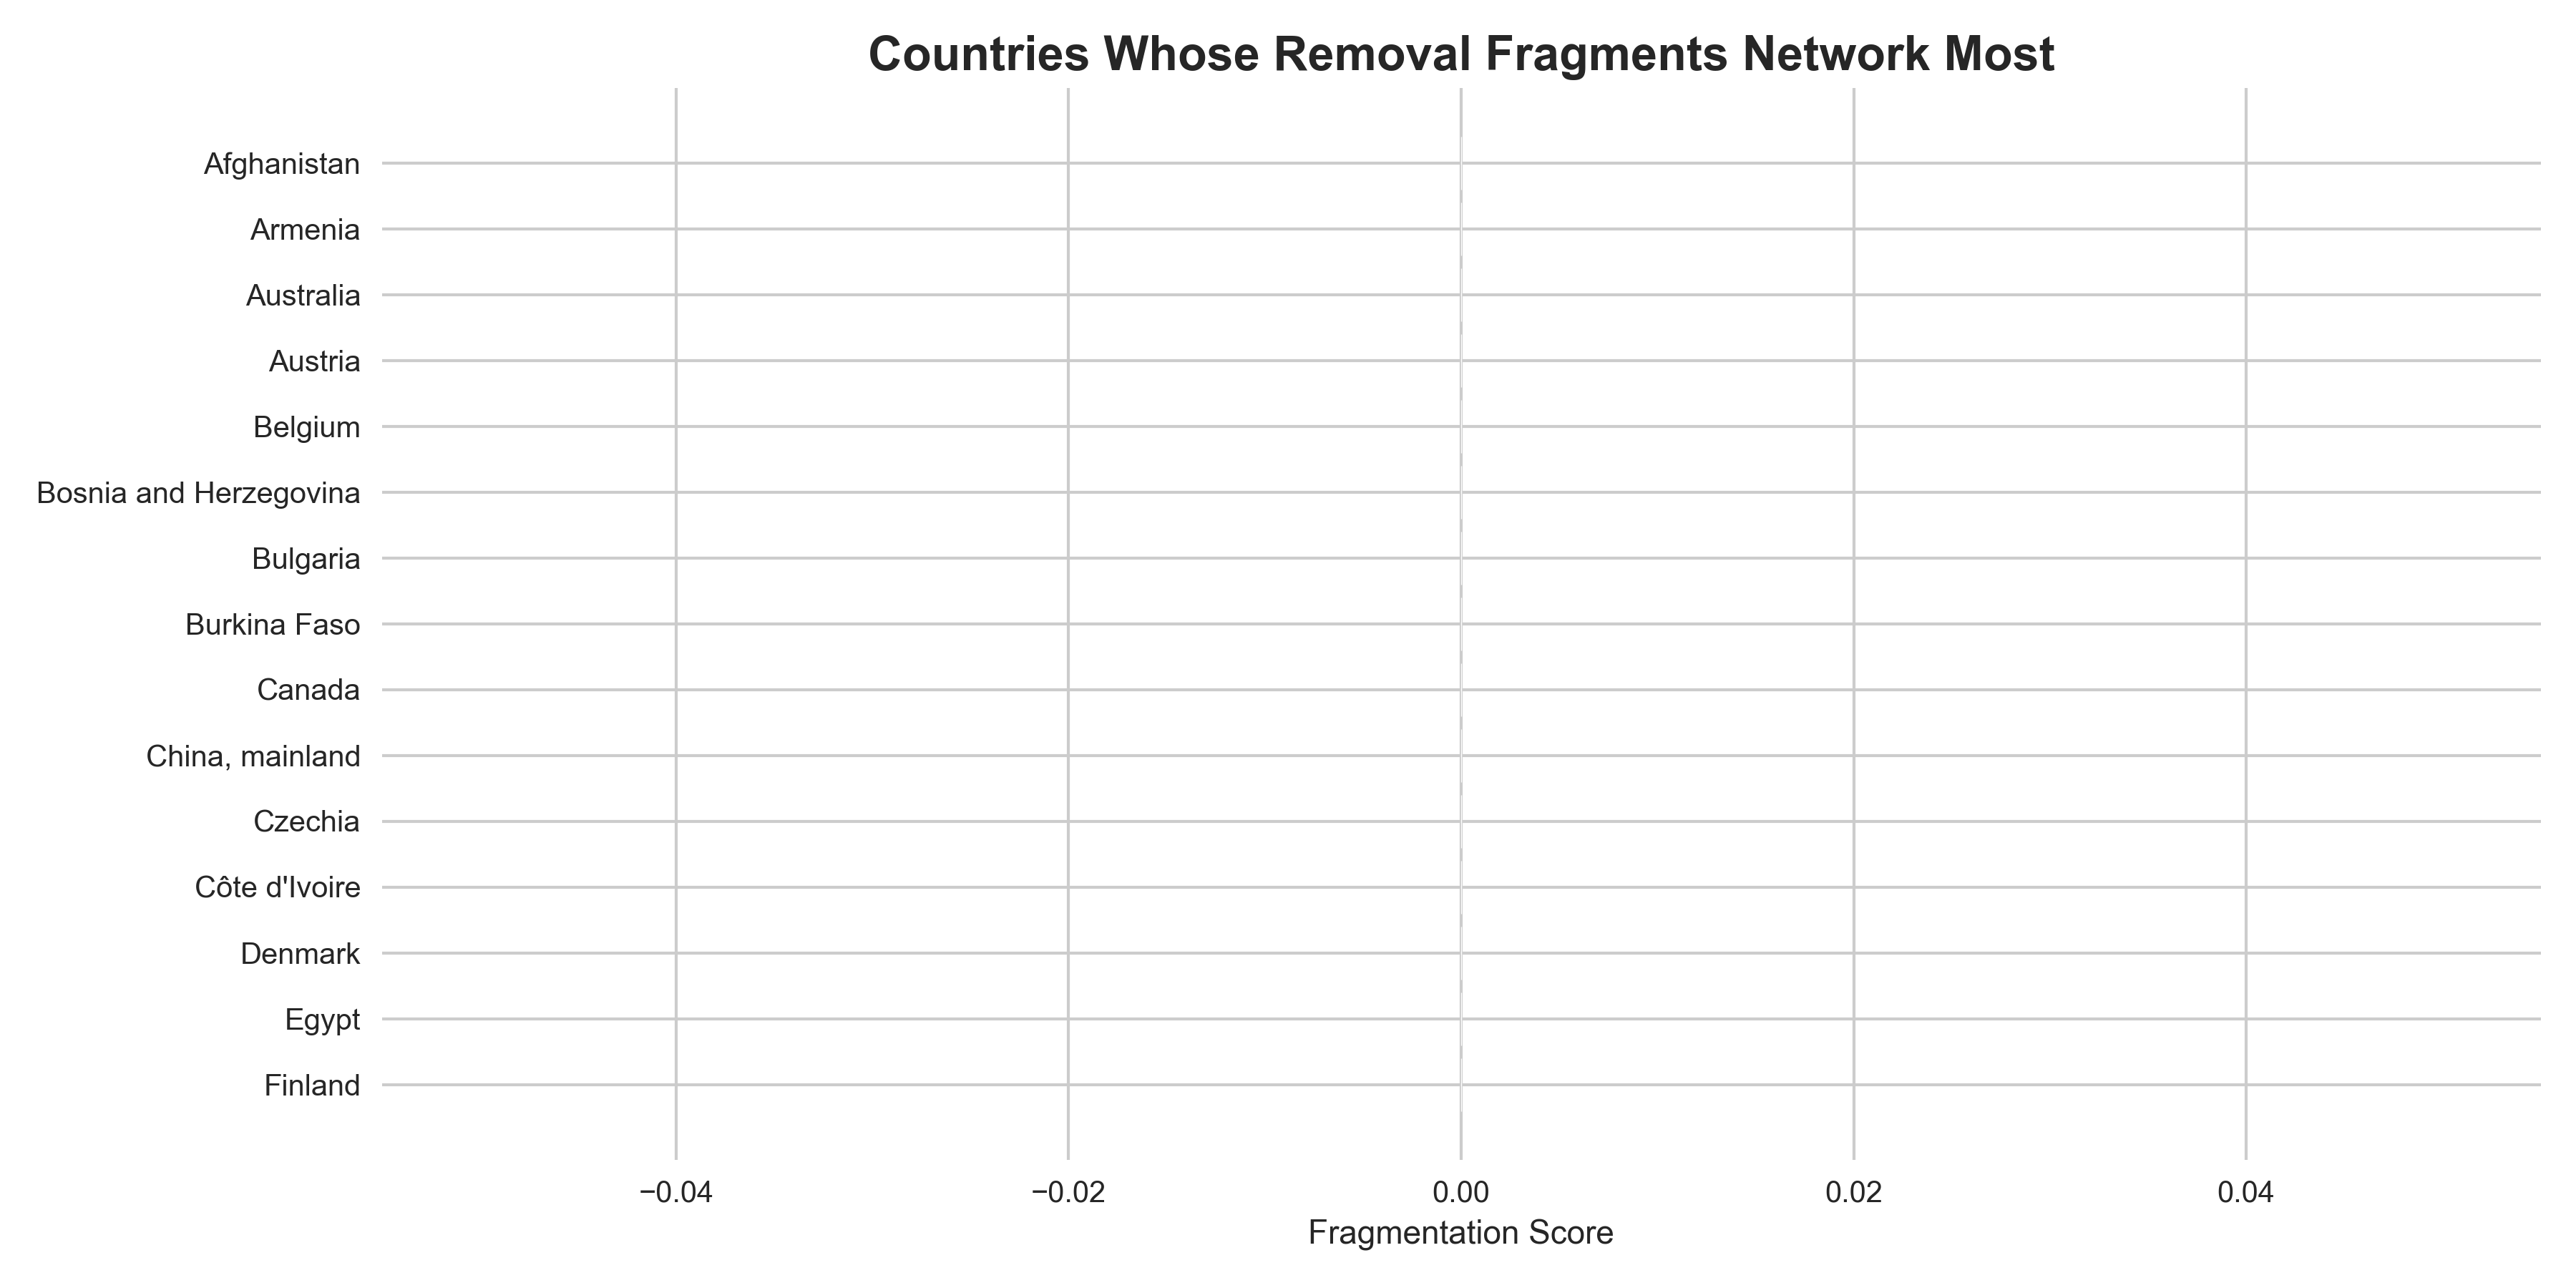
\includegraphics[width=\linewidth]{18_critical_countries.png}
    \caption{Structural critical countries (fragmentation impact).}
  \end{subfigure}
  \hfill
  \begin{subfigure}[t]{0.49\linewidth}
    \centering
    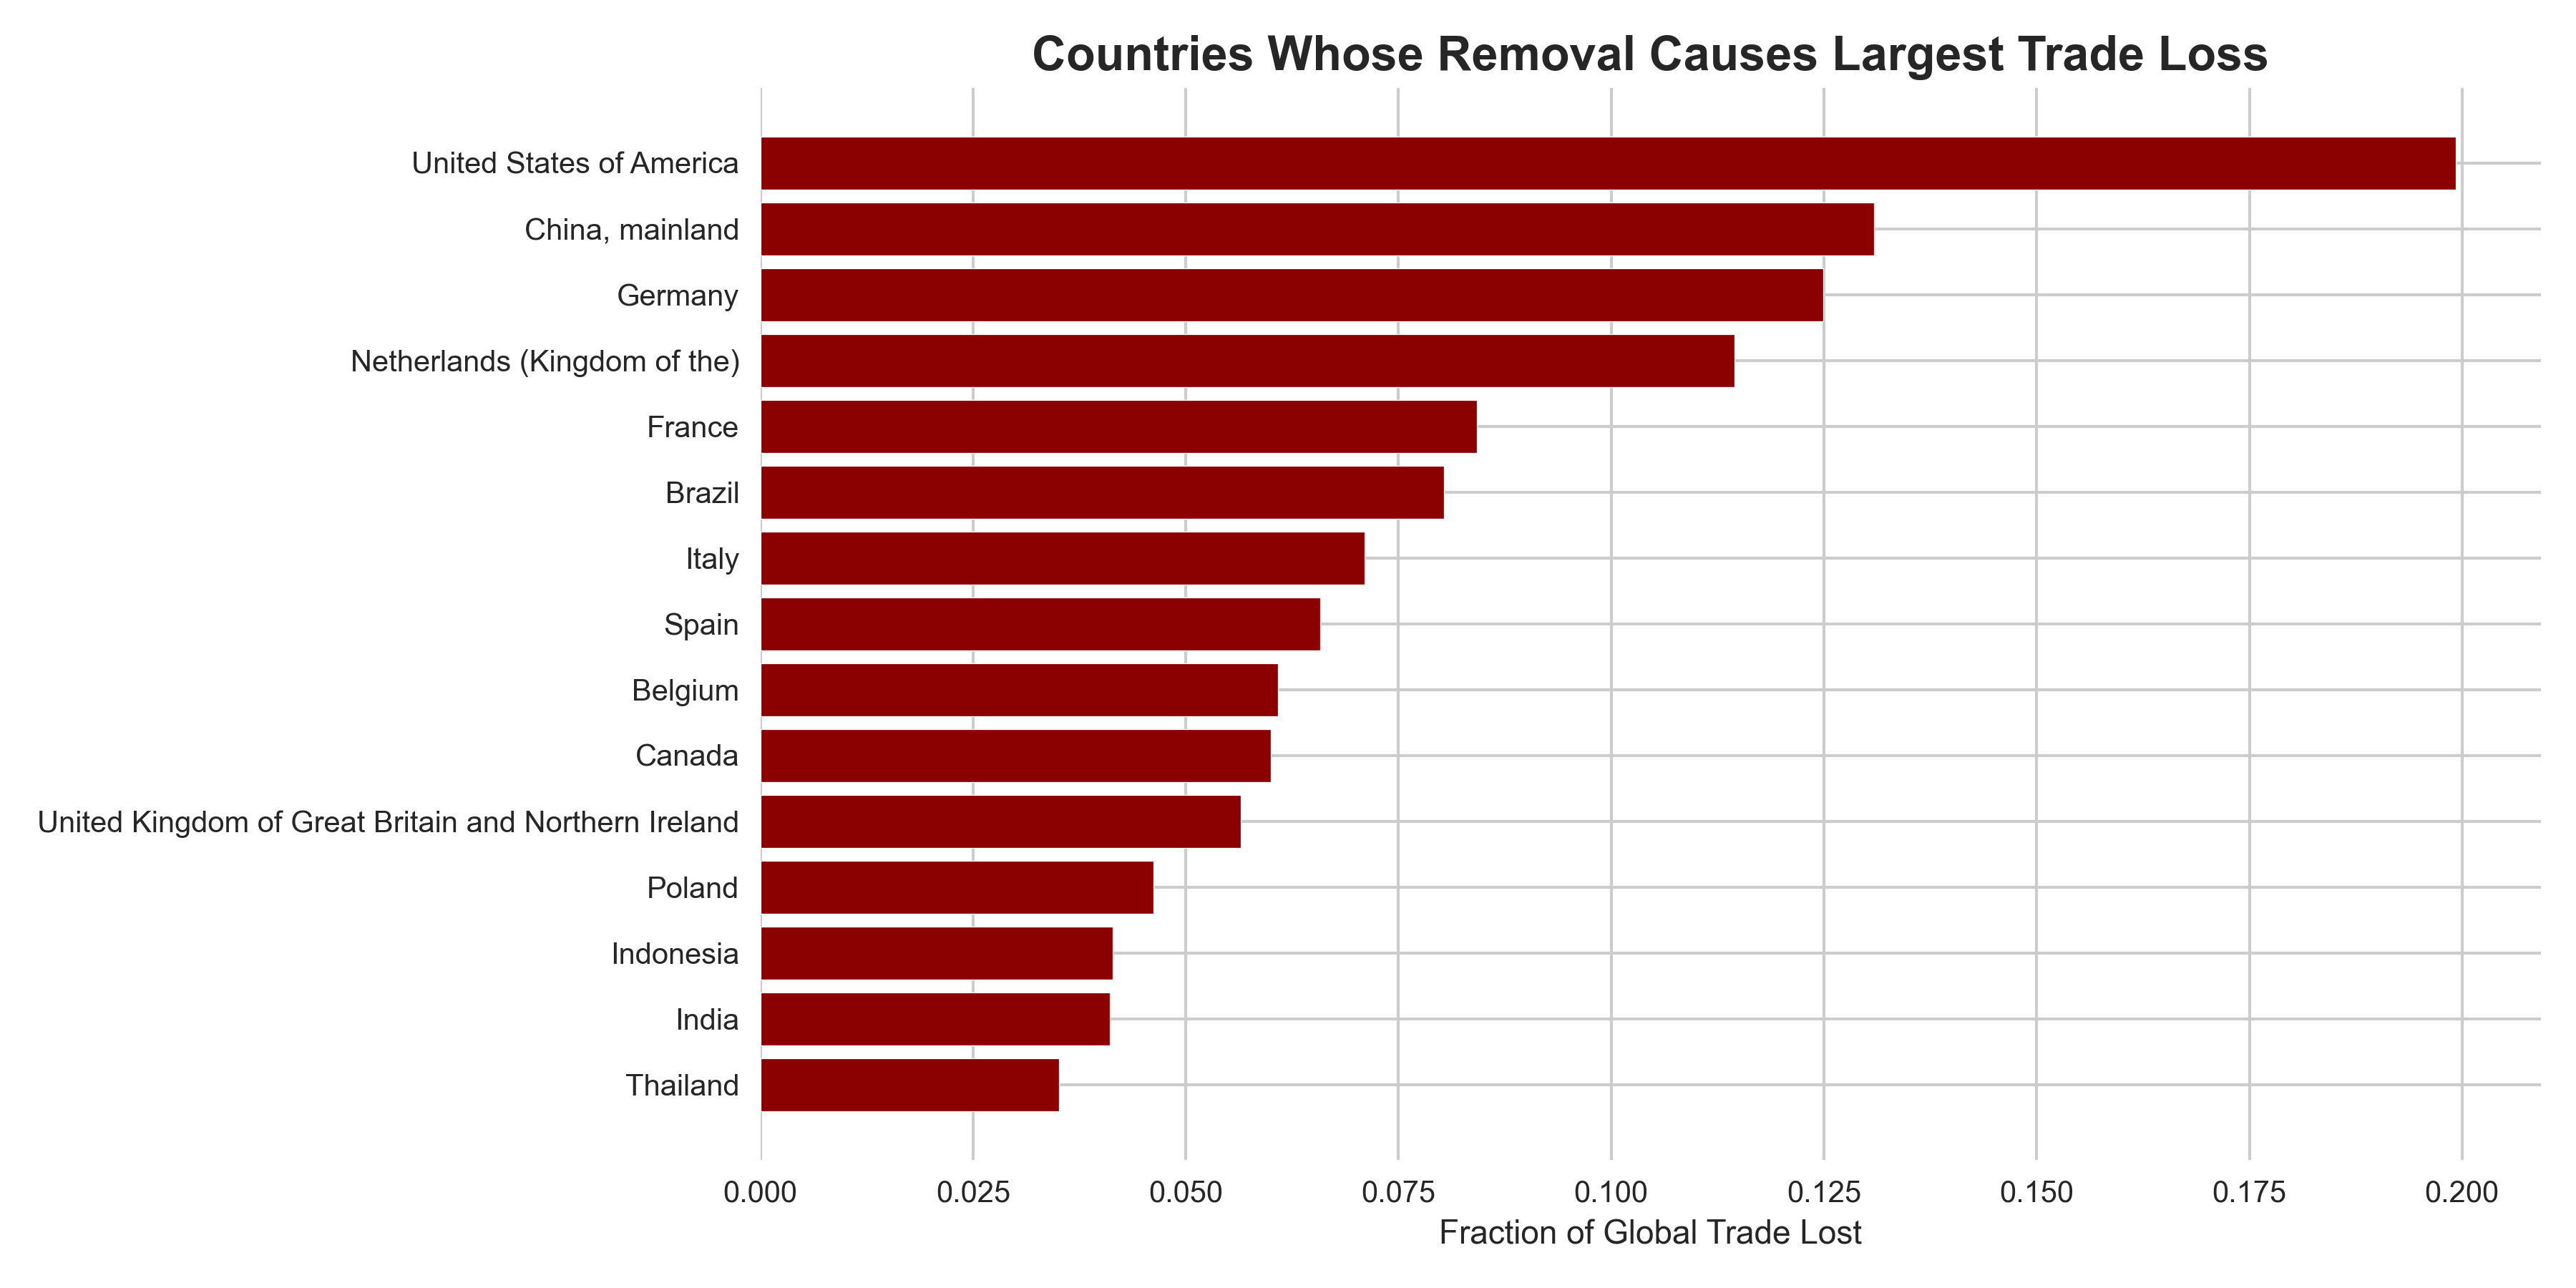
\includegraphics[width=\linewidth]{18b_weighted_critical_countries.png}
    \caption{Trade-value critical countries (flow-loss impact).}
  \end{subfigure}
  \caption{Critical countries differ depending on whether the objective is connectivity or trade value.}
  \label{fig:critical-countries}
\end{figure}

\begin{figure}[H]
  \centering
  \begin{subfigure}[t]{0.49\linewidth}
    \centering
    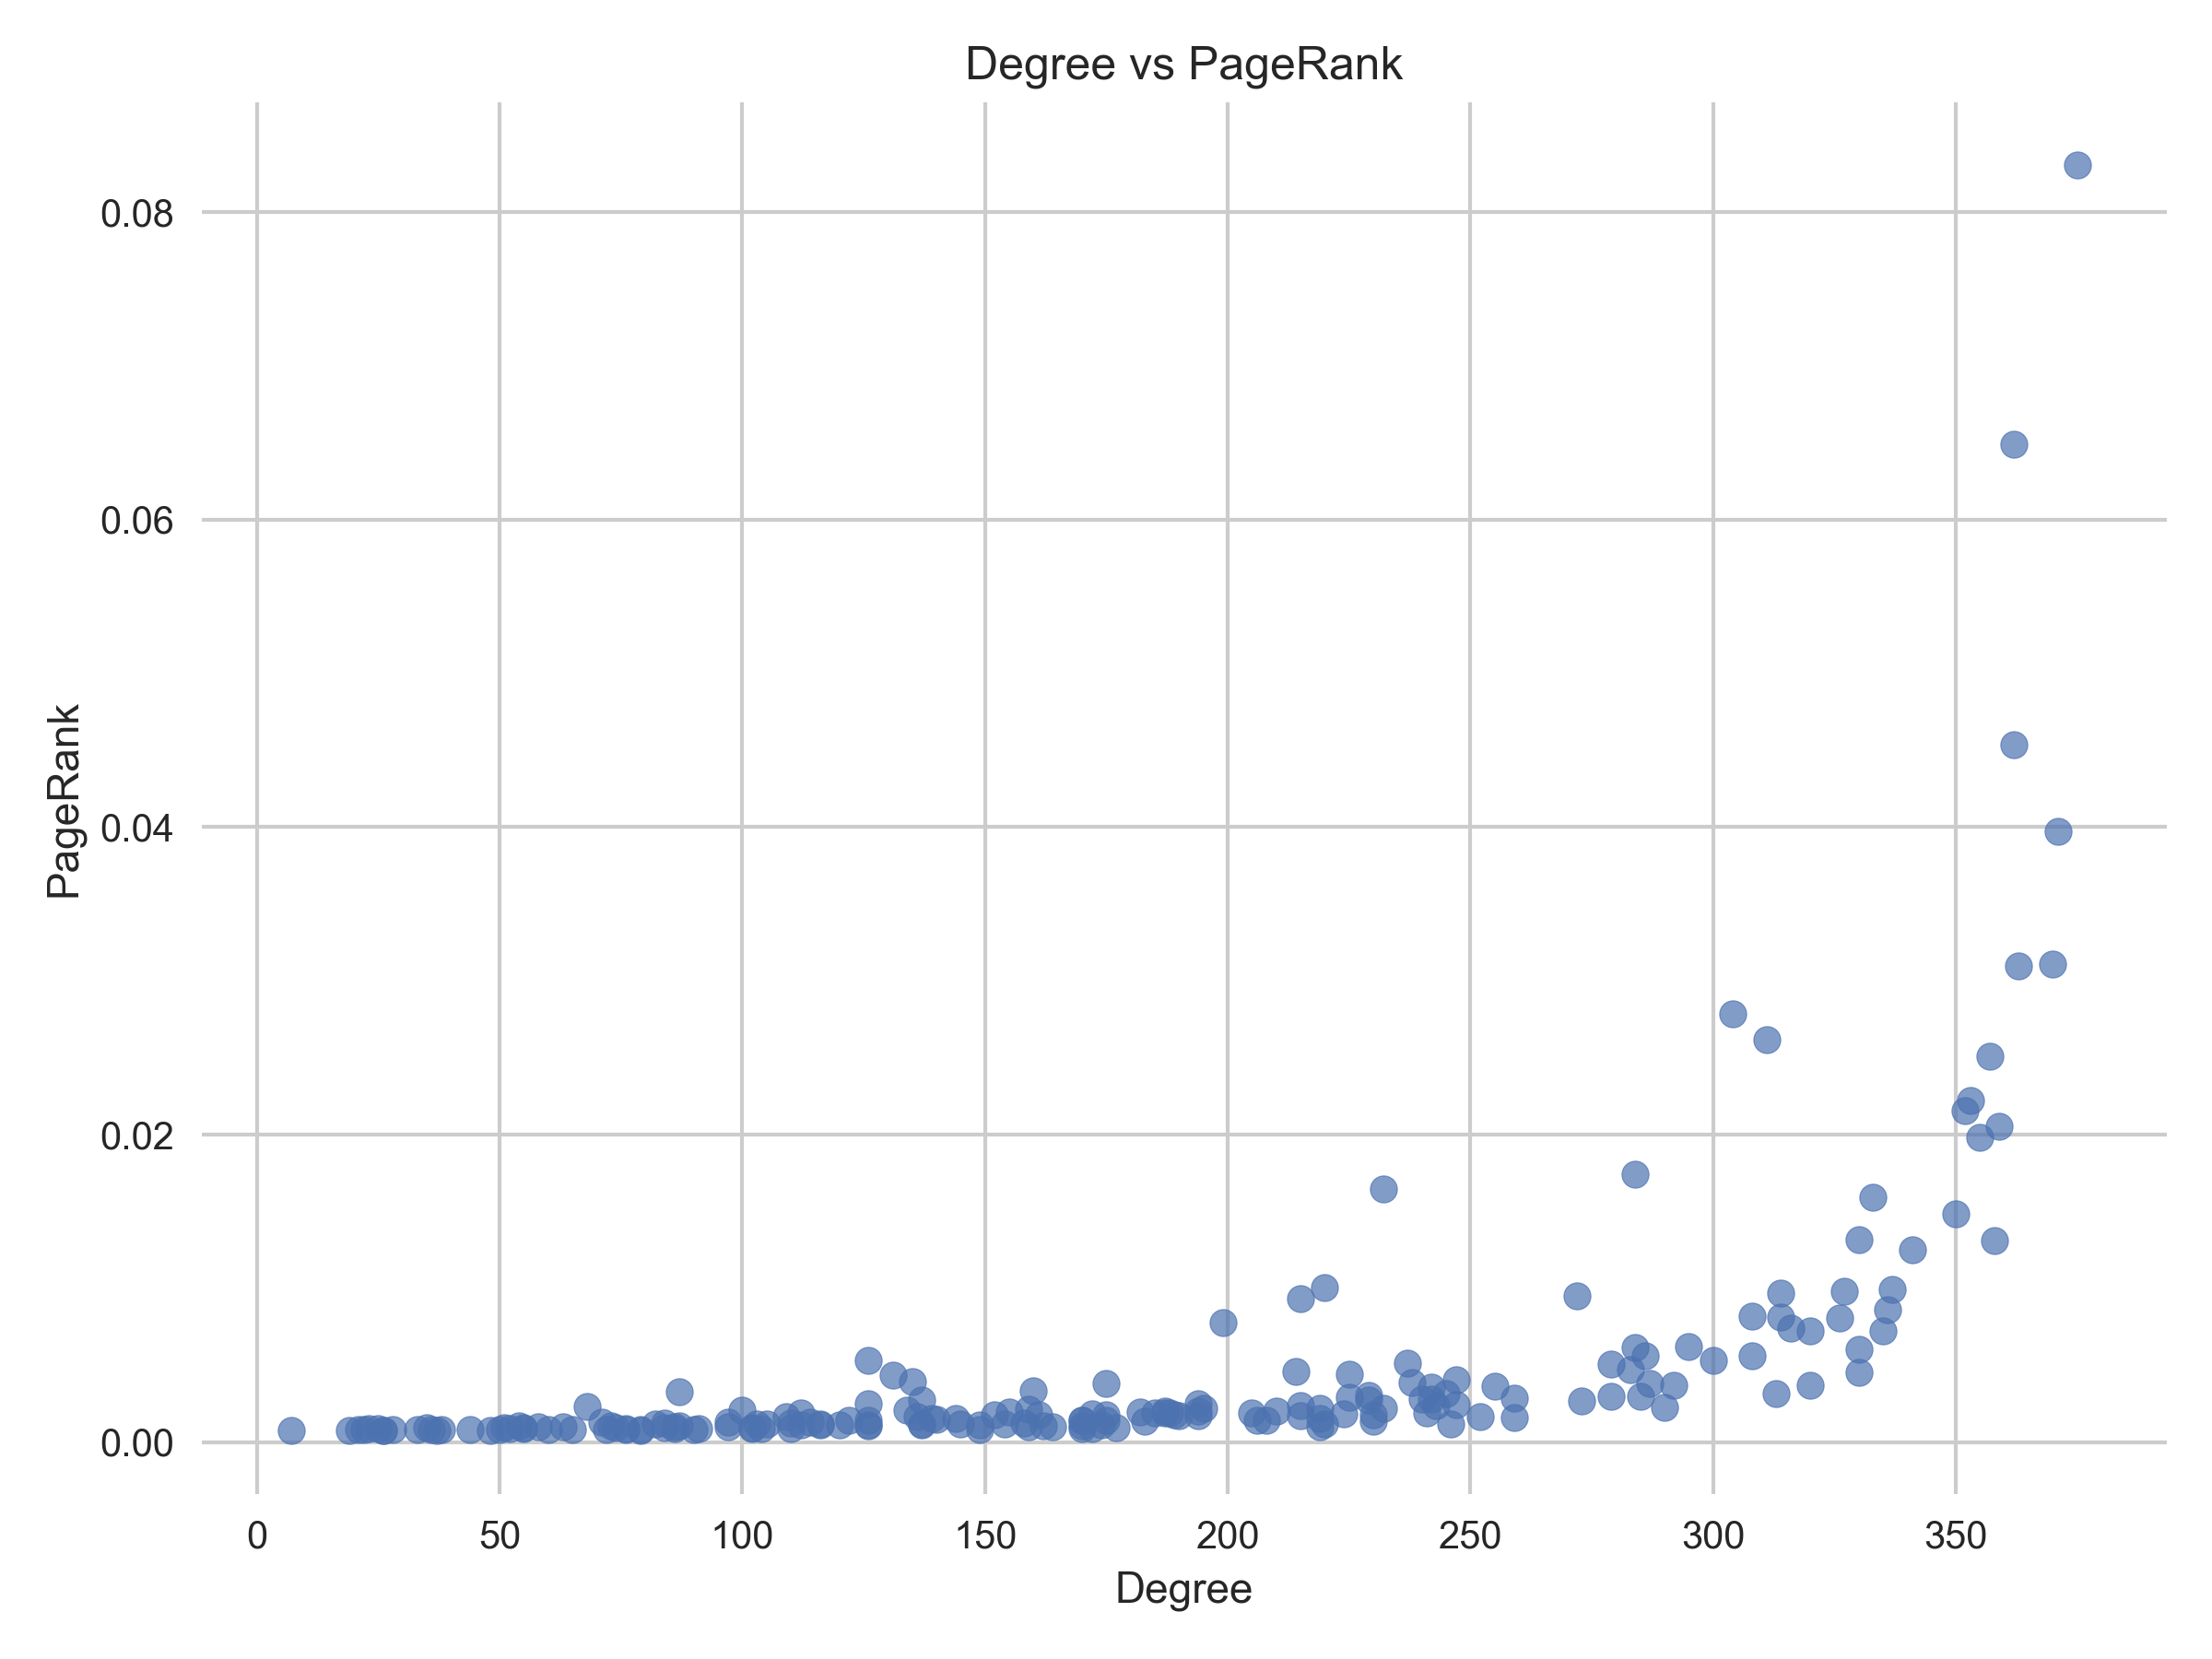
\includegraphics[width=\linewidth]{20_degree_vs_pagerank.png}
    \caption{Degree vs PageRank: connectivity vs influence.}
  \end{subfigure}
  \hfill
  \begin{subfigure}[t]{0.49\linewidth}
    \centering
    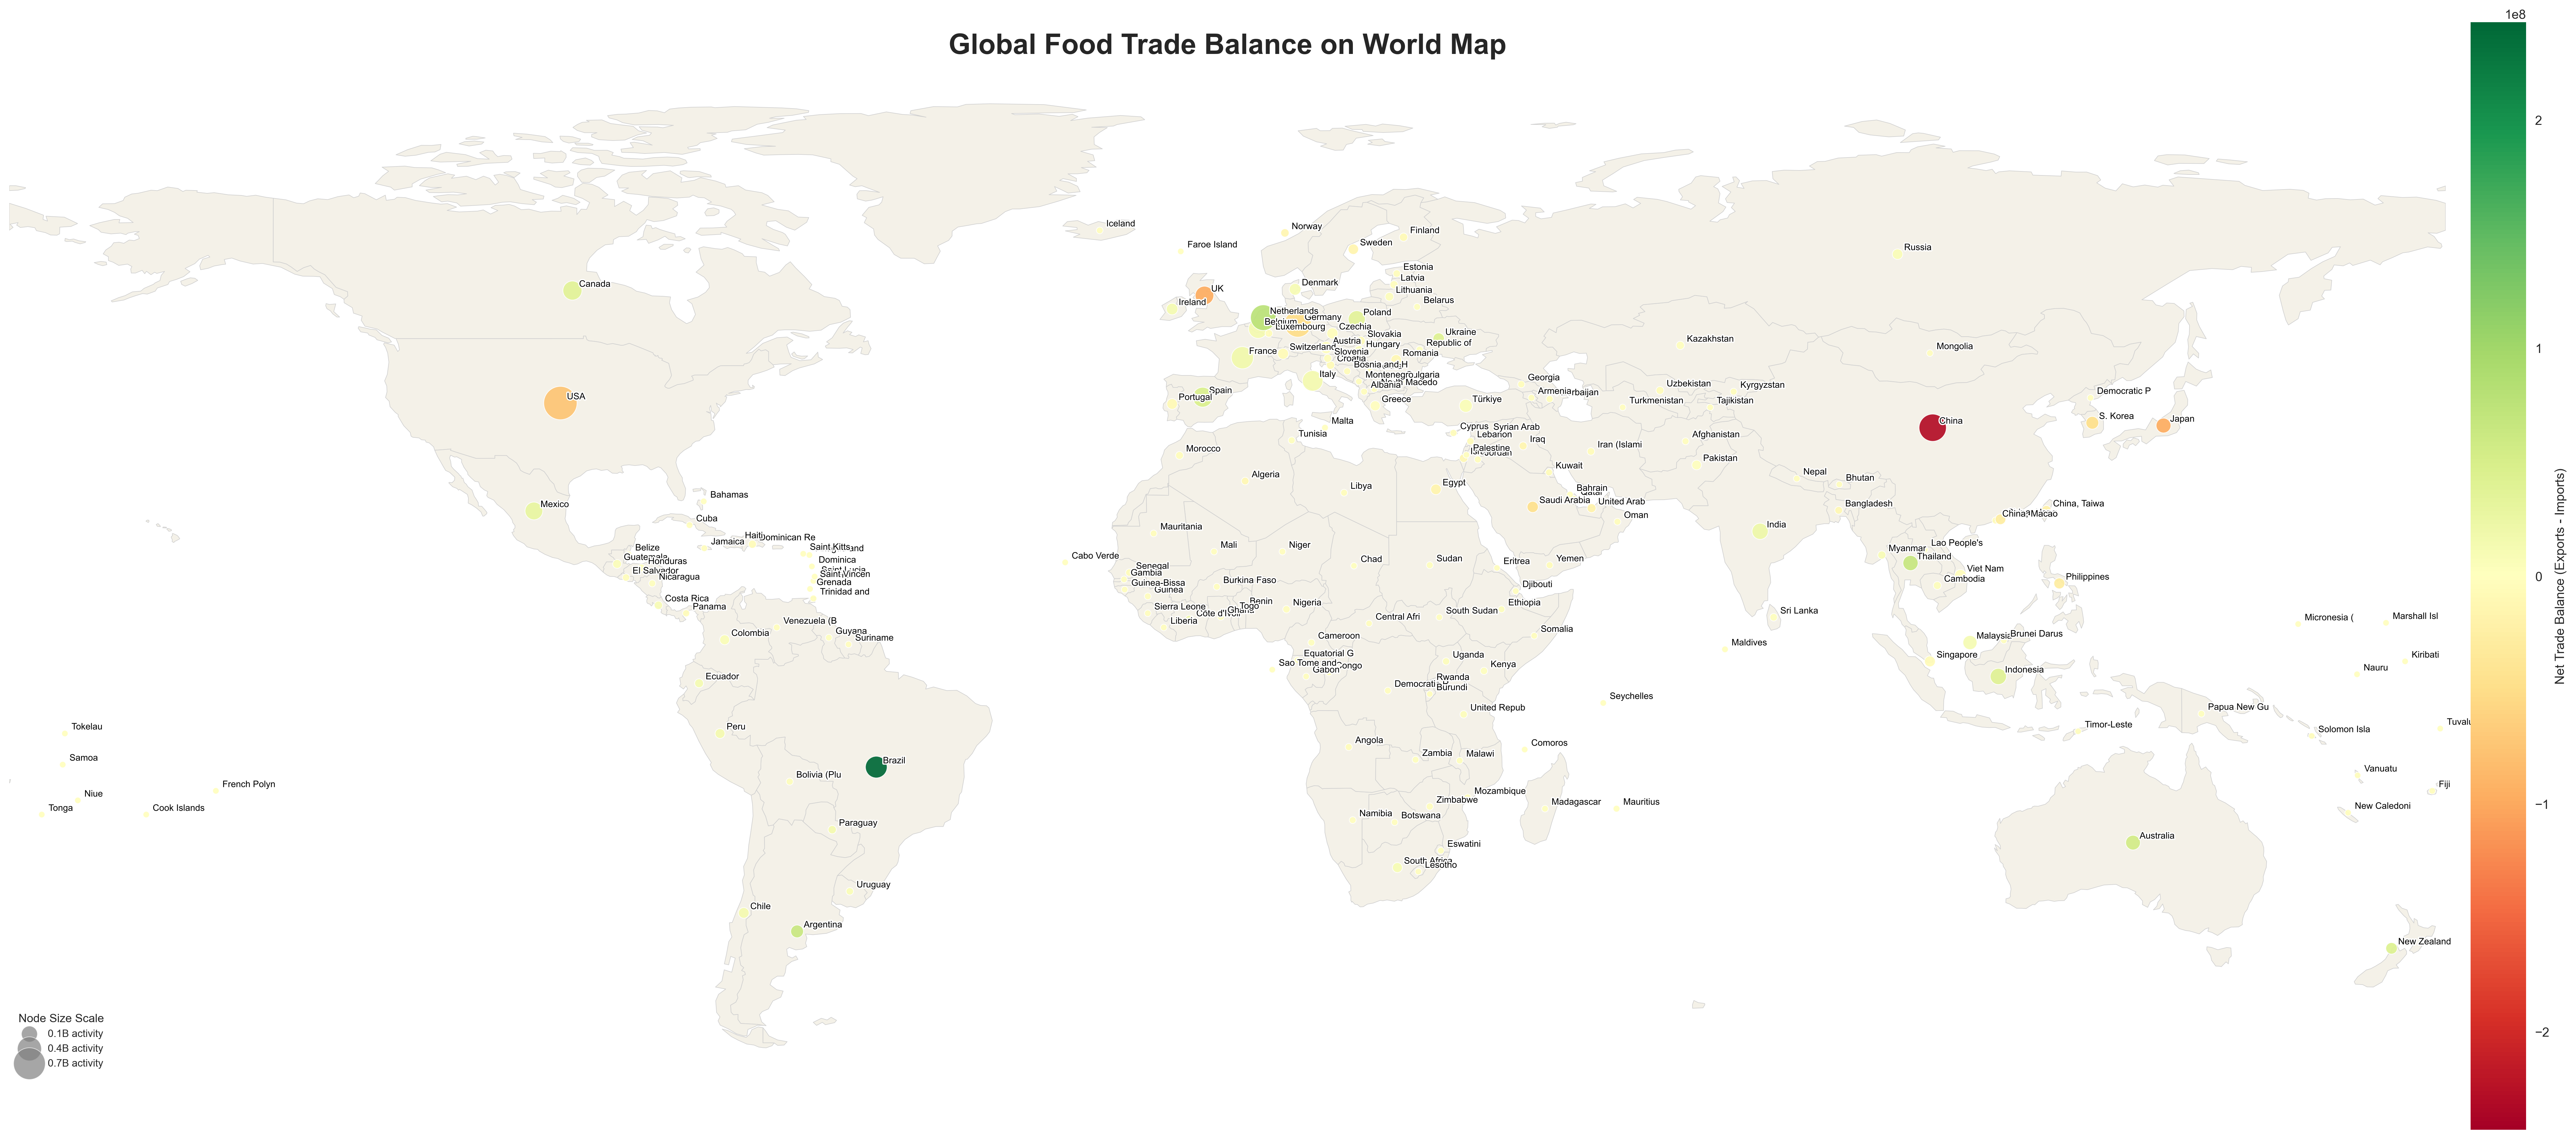
\includegraphics[width=\linewidth]{40_world_map_trade_balance.png}
    \caption{Trade balance (map): net exporters vs net importers.}
  \end{subfigure}
  \caption{Supporting views of structural position and net trade balance.}
  \label{fig:supporting}
\end{figure}

\begin{figure}[H]
  \centering
  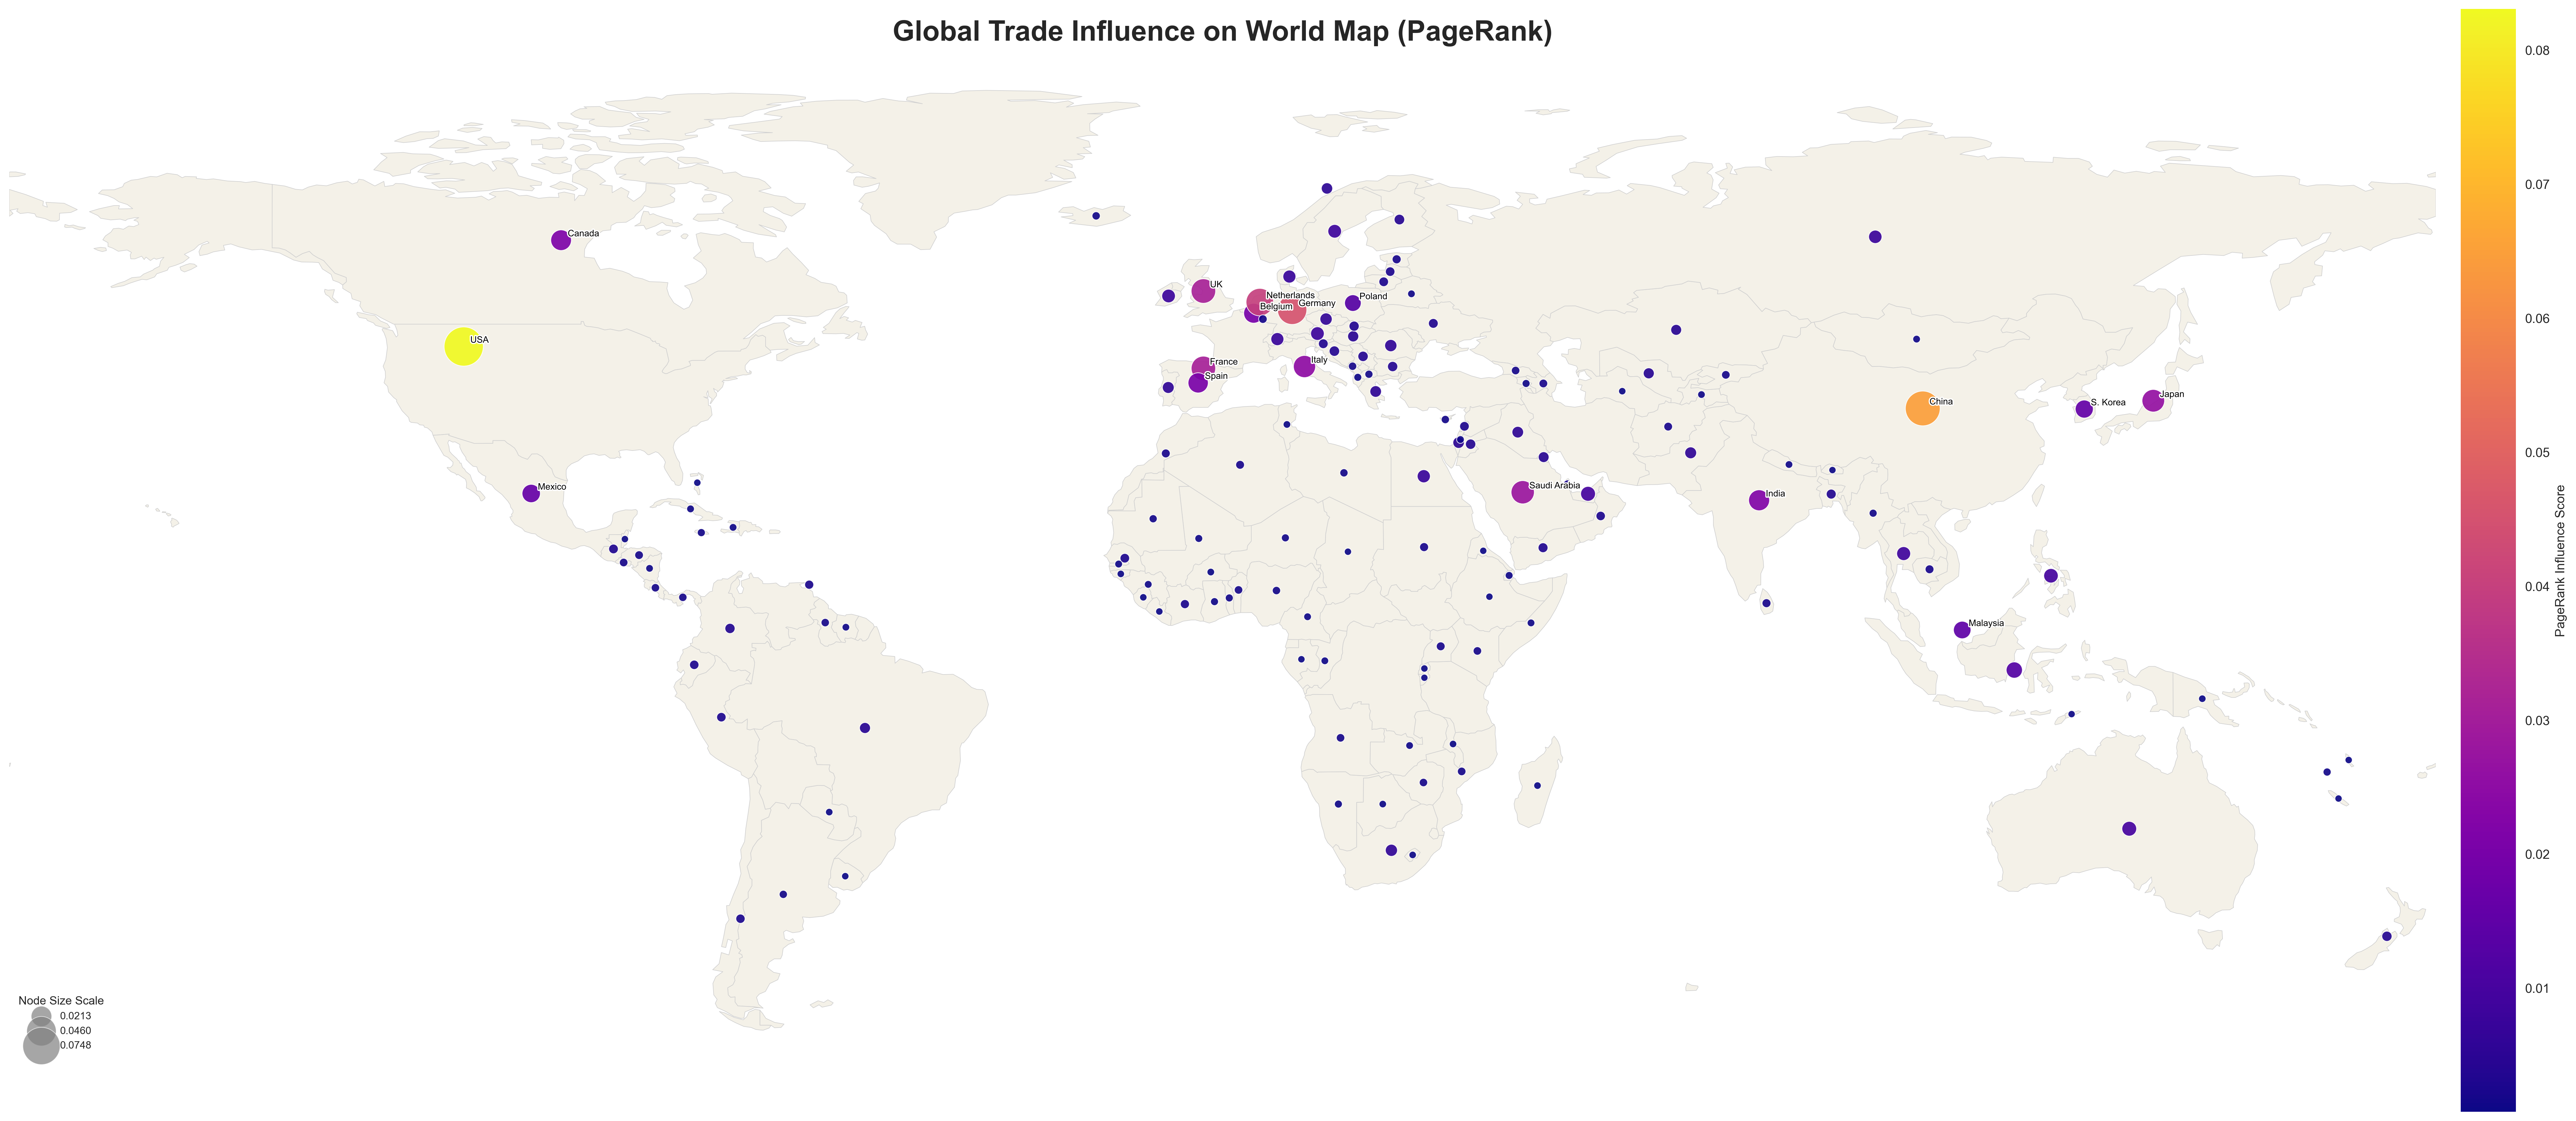
\includegraphics[width=0.98\linewidth]{39_world_map_pagerank.png}
  \caption{Influence mapped geographically (PageRank).}
  \label{fig:pagerank-map}
\end{figure}

\paragraph{Critical country takeaways.}
\begin{itemize}
  \item Power comes from network position, not only trade volume.
  \item Bridge countries can be system-critical even if not top exporters/importers.
  \item Targeted removal of a small set of top-ranked countries causes rapid systemic damage.
  \item Structural and weighted criticality are related but not identical.
\end{itemize}

\section{Fragility: Random Failures vs Targeted Attacks}
\subsection{Connectivity collapse}
\begin{figure}[H]
  \centering
  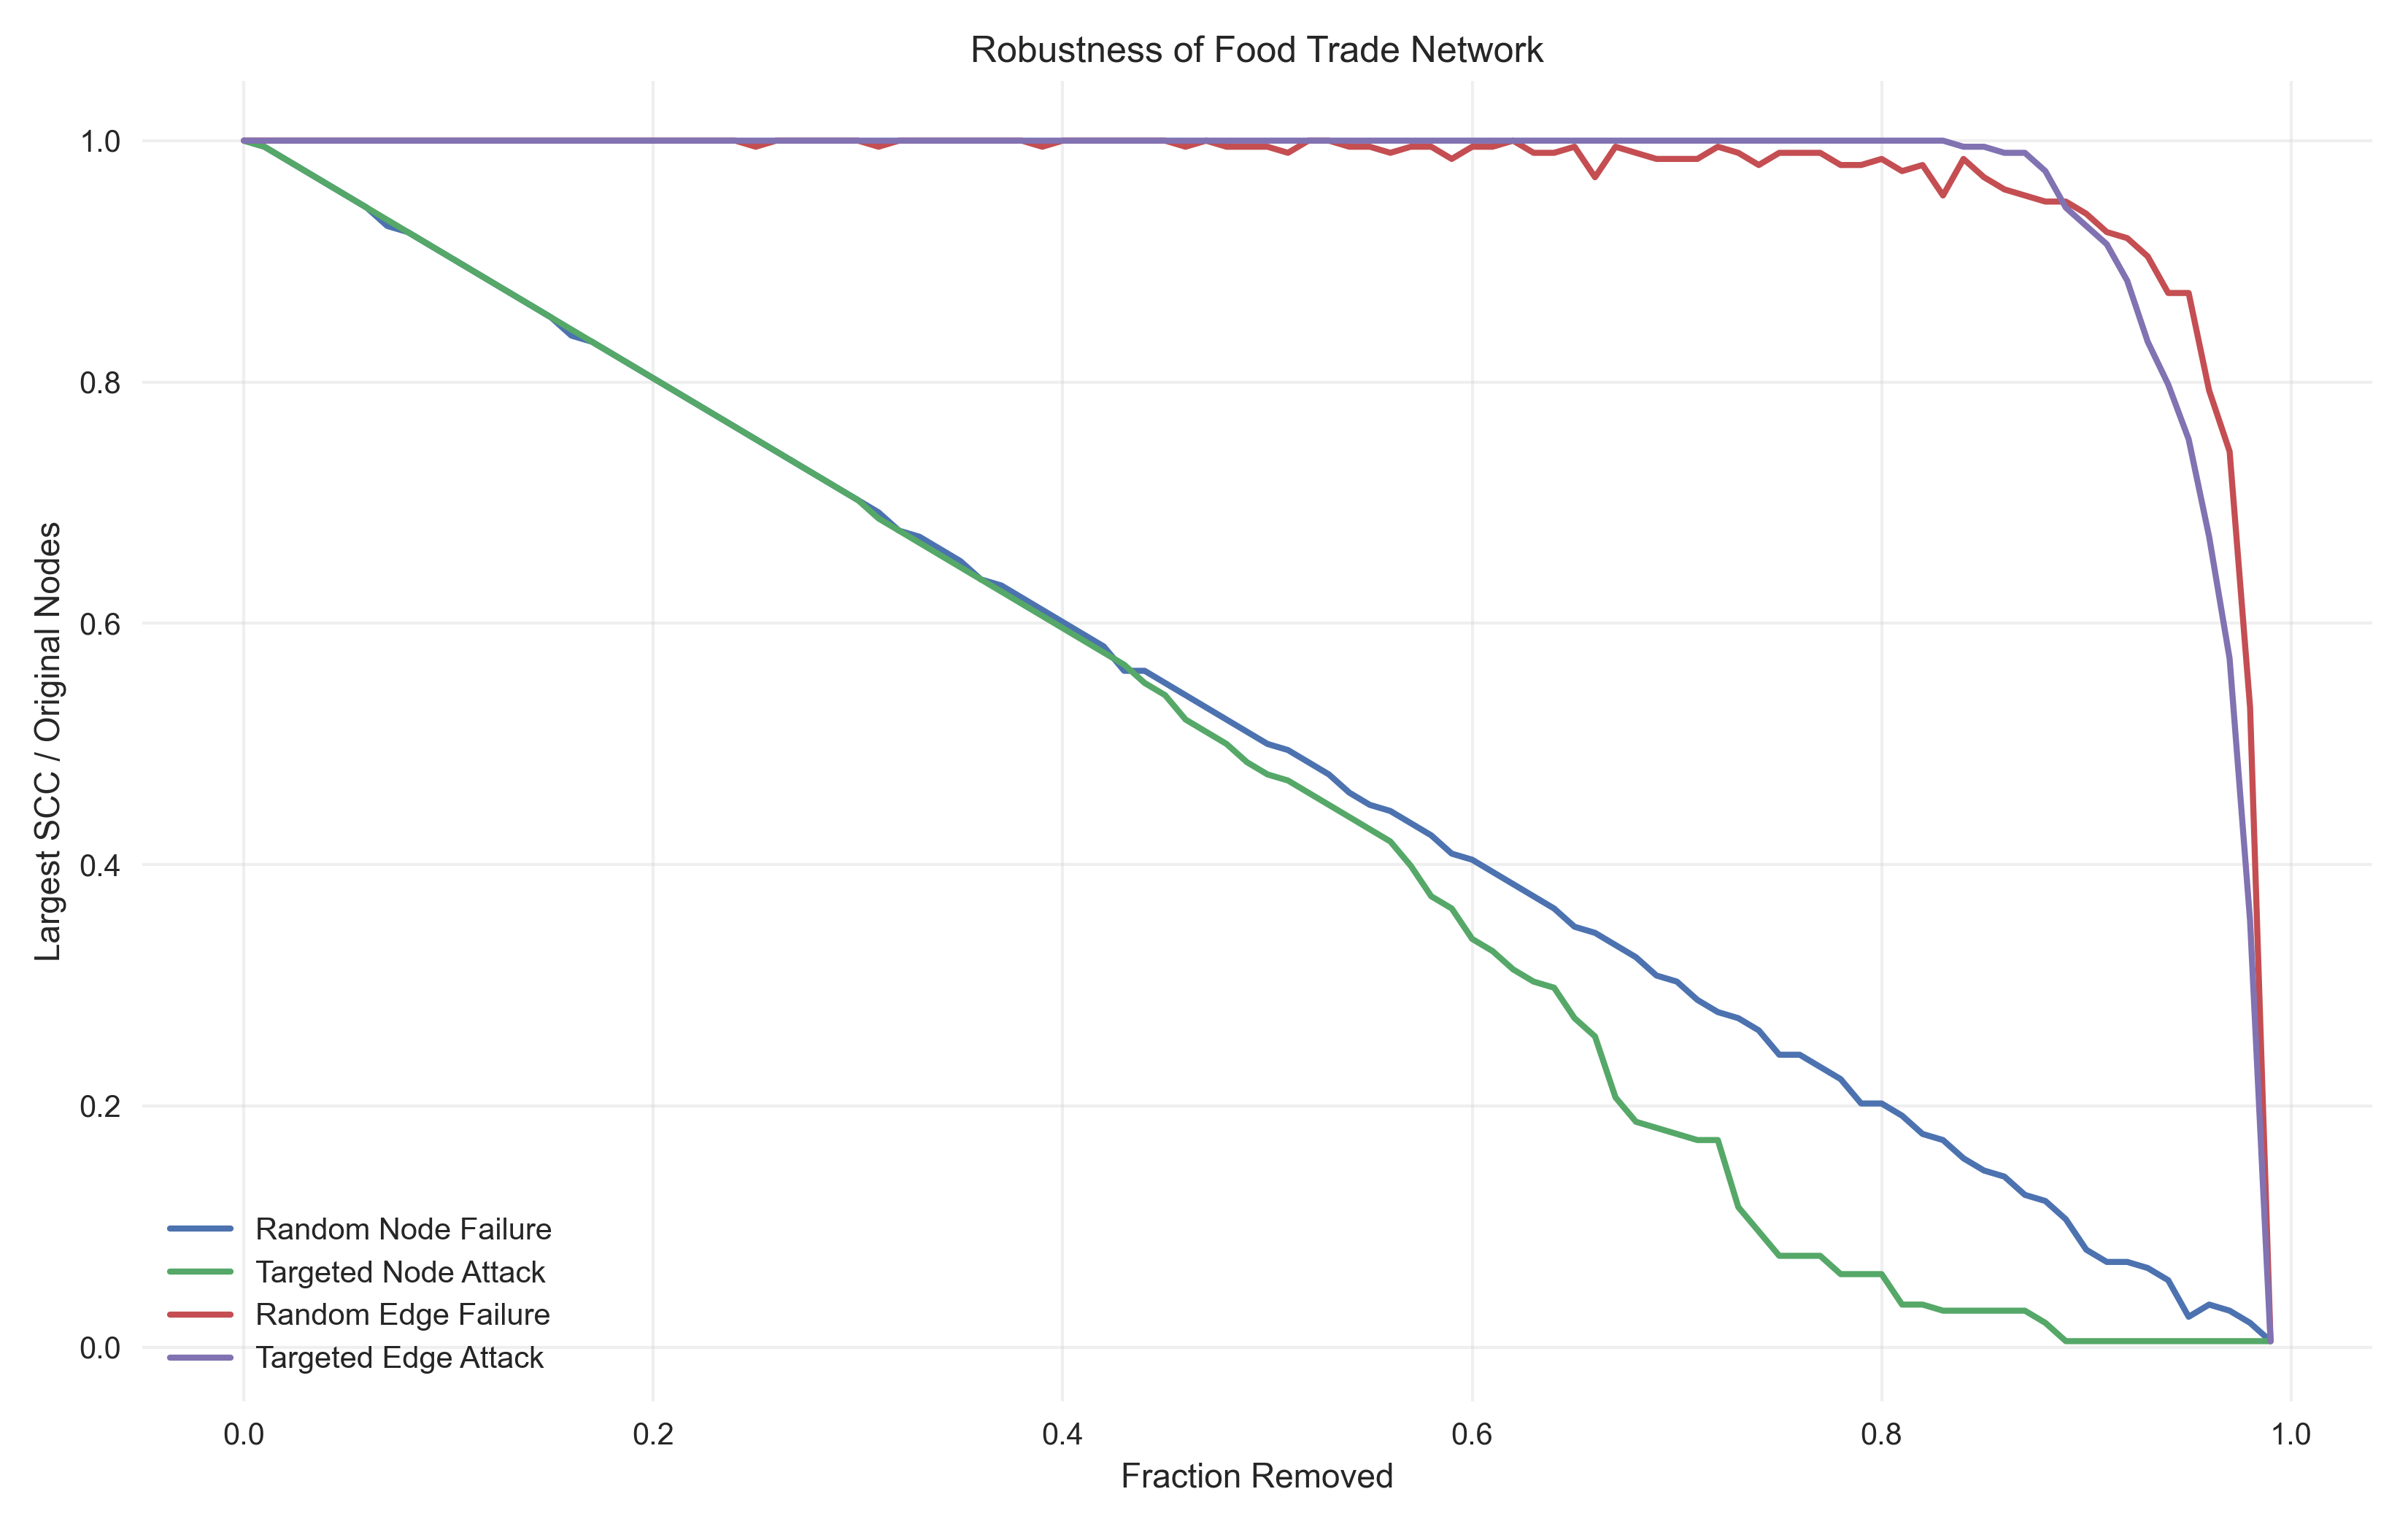
\includegraphics[width=0.98\linewidth]{23_full_robustness.png}
  \caption{Largest strongly connected component under attacks. Random failures degrade gradually; targeted removal triggers rapid collapse after a threshold.}
  \label{fig:robustness-connectivity}
\end{figure}

\subsection{Trade-value collapse}
\begin{figure}[H]
  \centering
  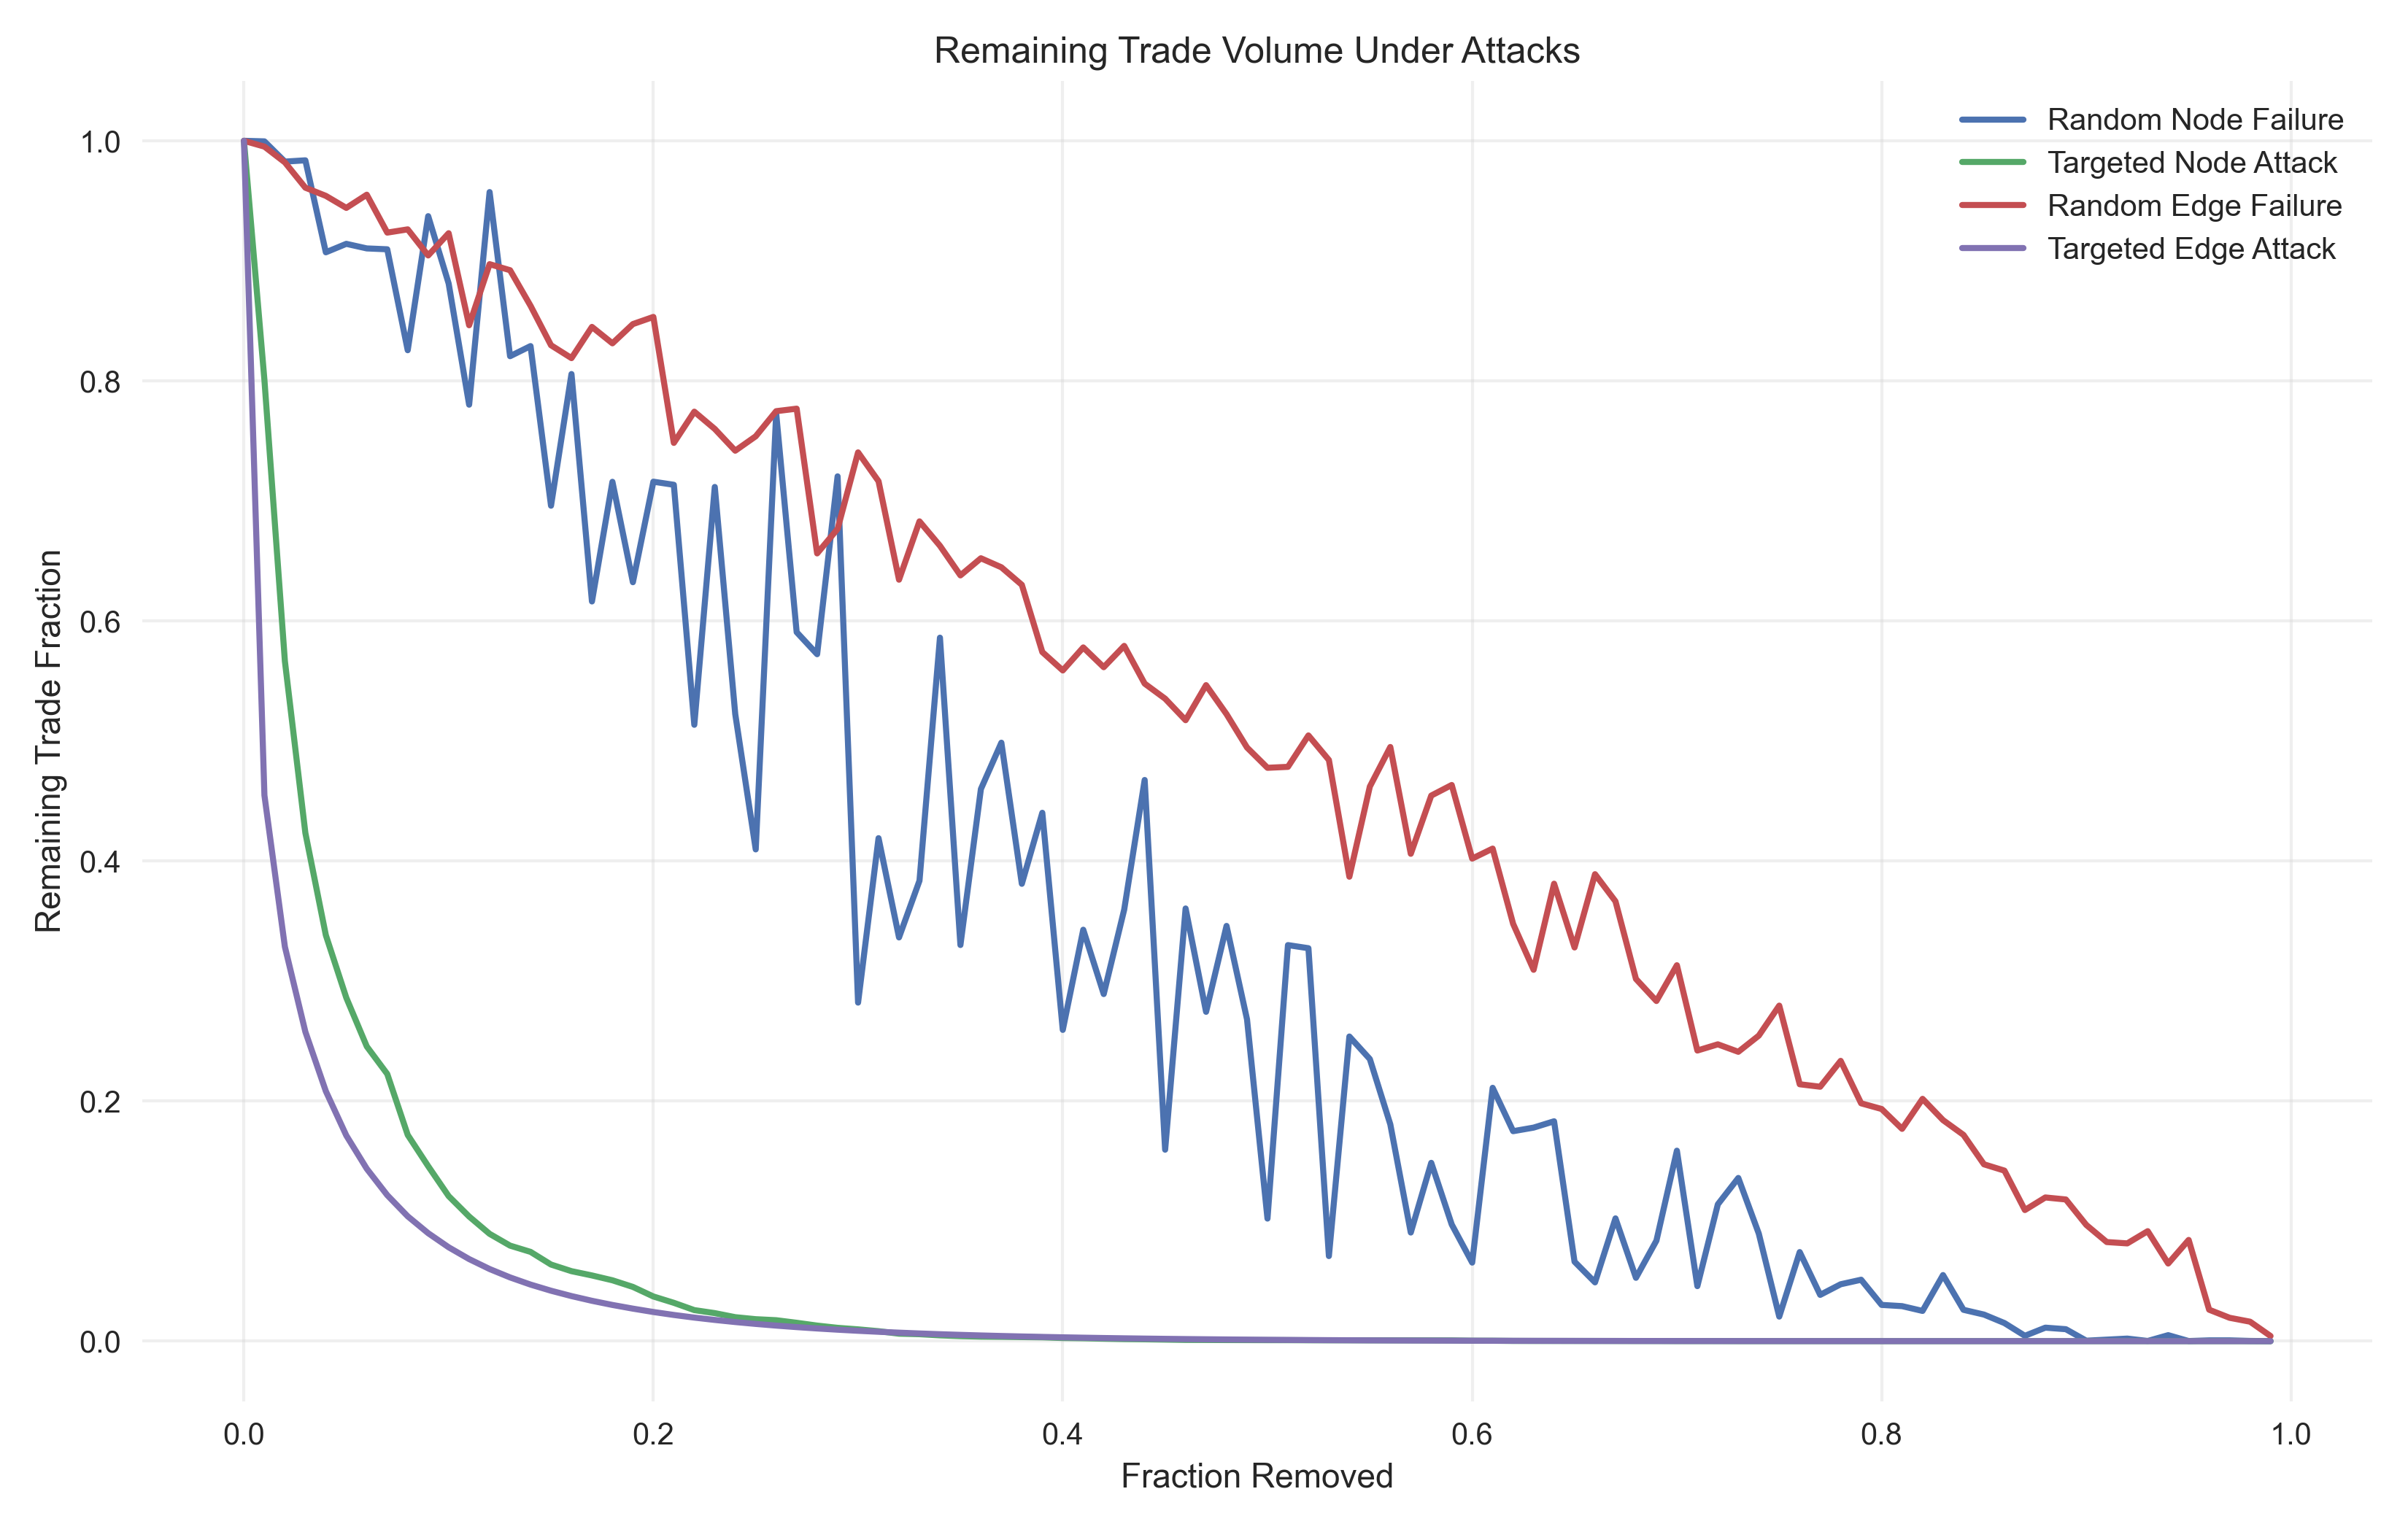
\includegraphics[width=0.98\linewidth]{23b_trade_robustness.png}
  \caption{Remaining trade value under attacks. Targeted strategies eliminate value much faster than random removal.}
  \label{fig:robustness-trade}
\end{figure}

\subsection{Weighted damage curves}
\begin{figure}[H]
  \centering
  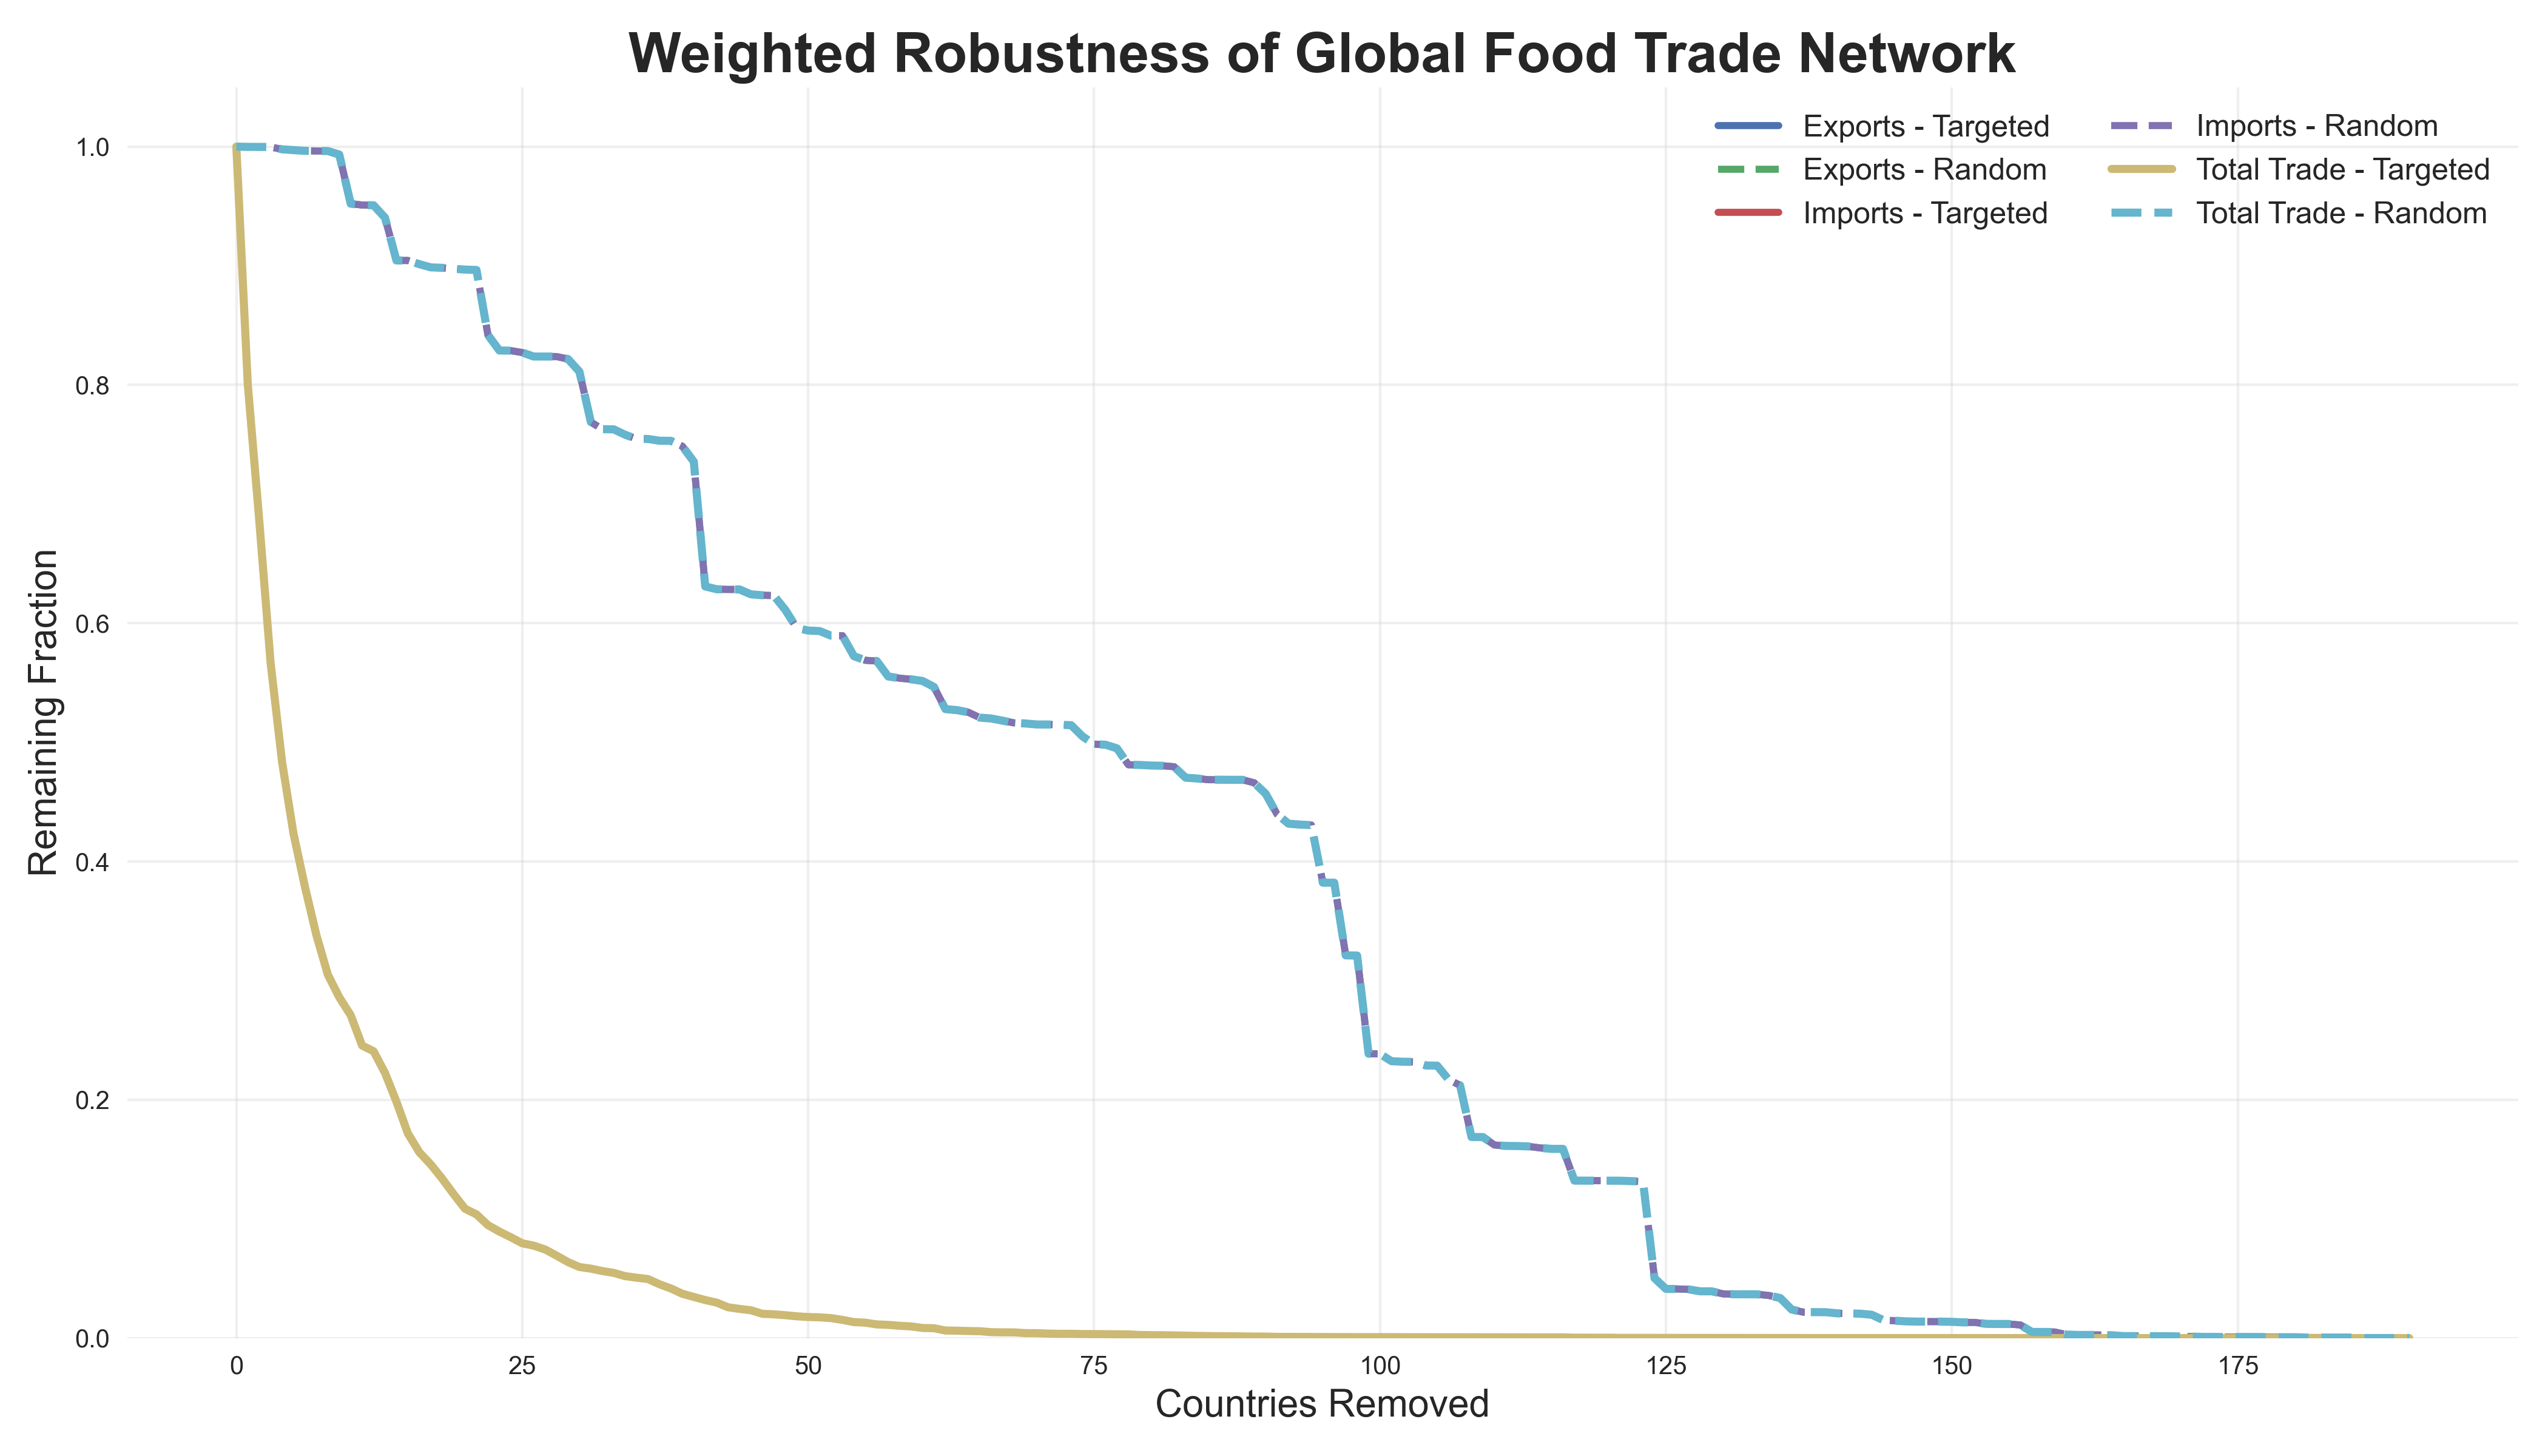
\includegraphics[width=0.98\linewidth]{39_weighted_robustness_combined.png}
  \caption{Weighted robustness summary: exports, imports, and total trade under random vs targeted removal.}
  \label{fig:weighted-robustness}
\end{figure}

\subsection{Exposure and mitigation}
\begin{figure}[H]
  \centering
  \begin{subfigure}[t]{0.49\linewidth}
    \centering
    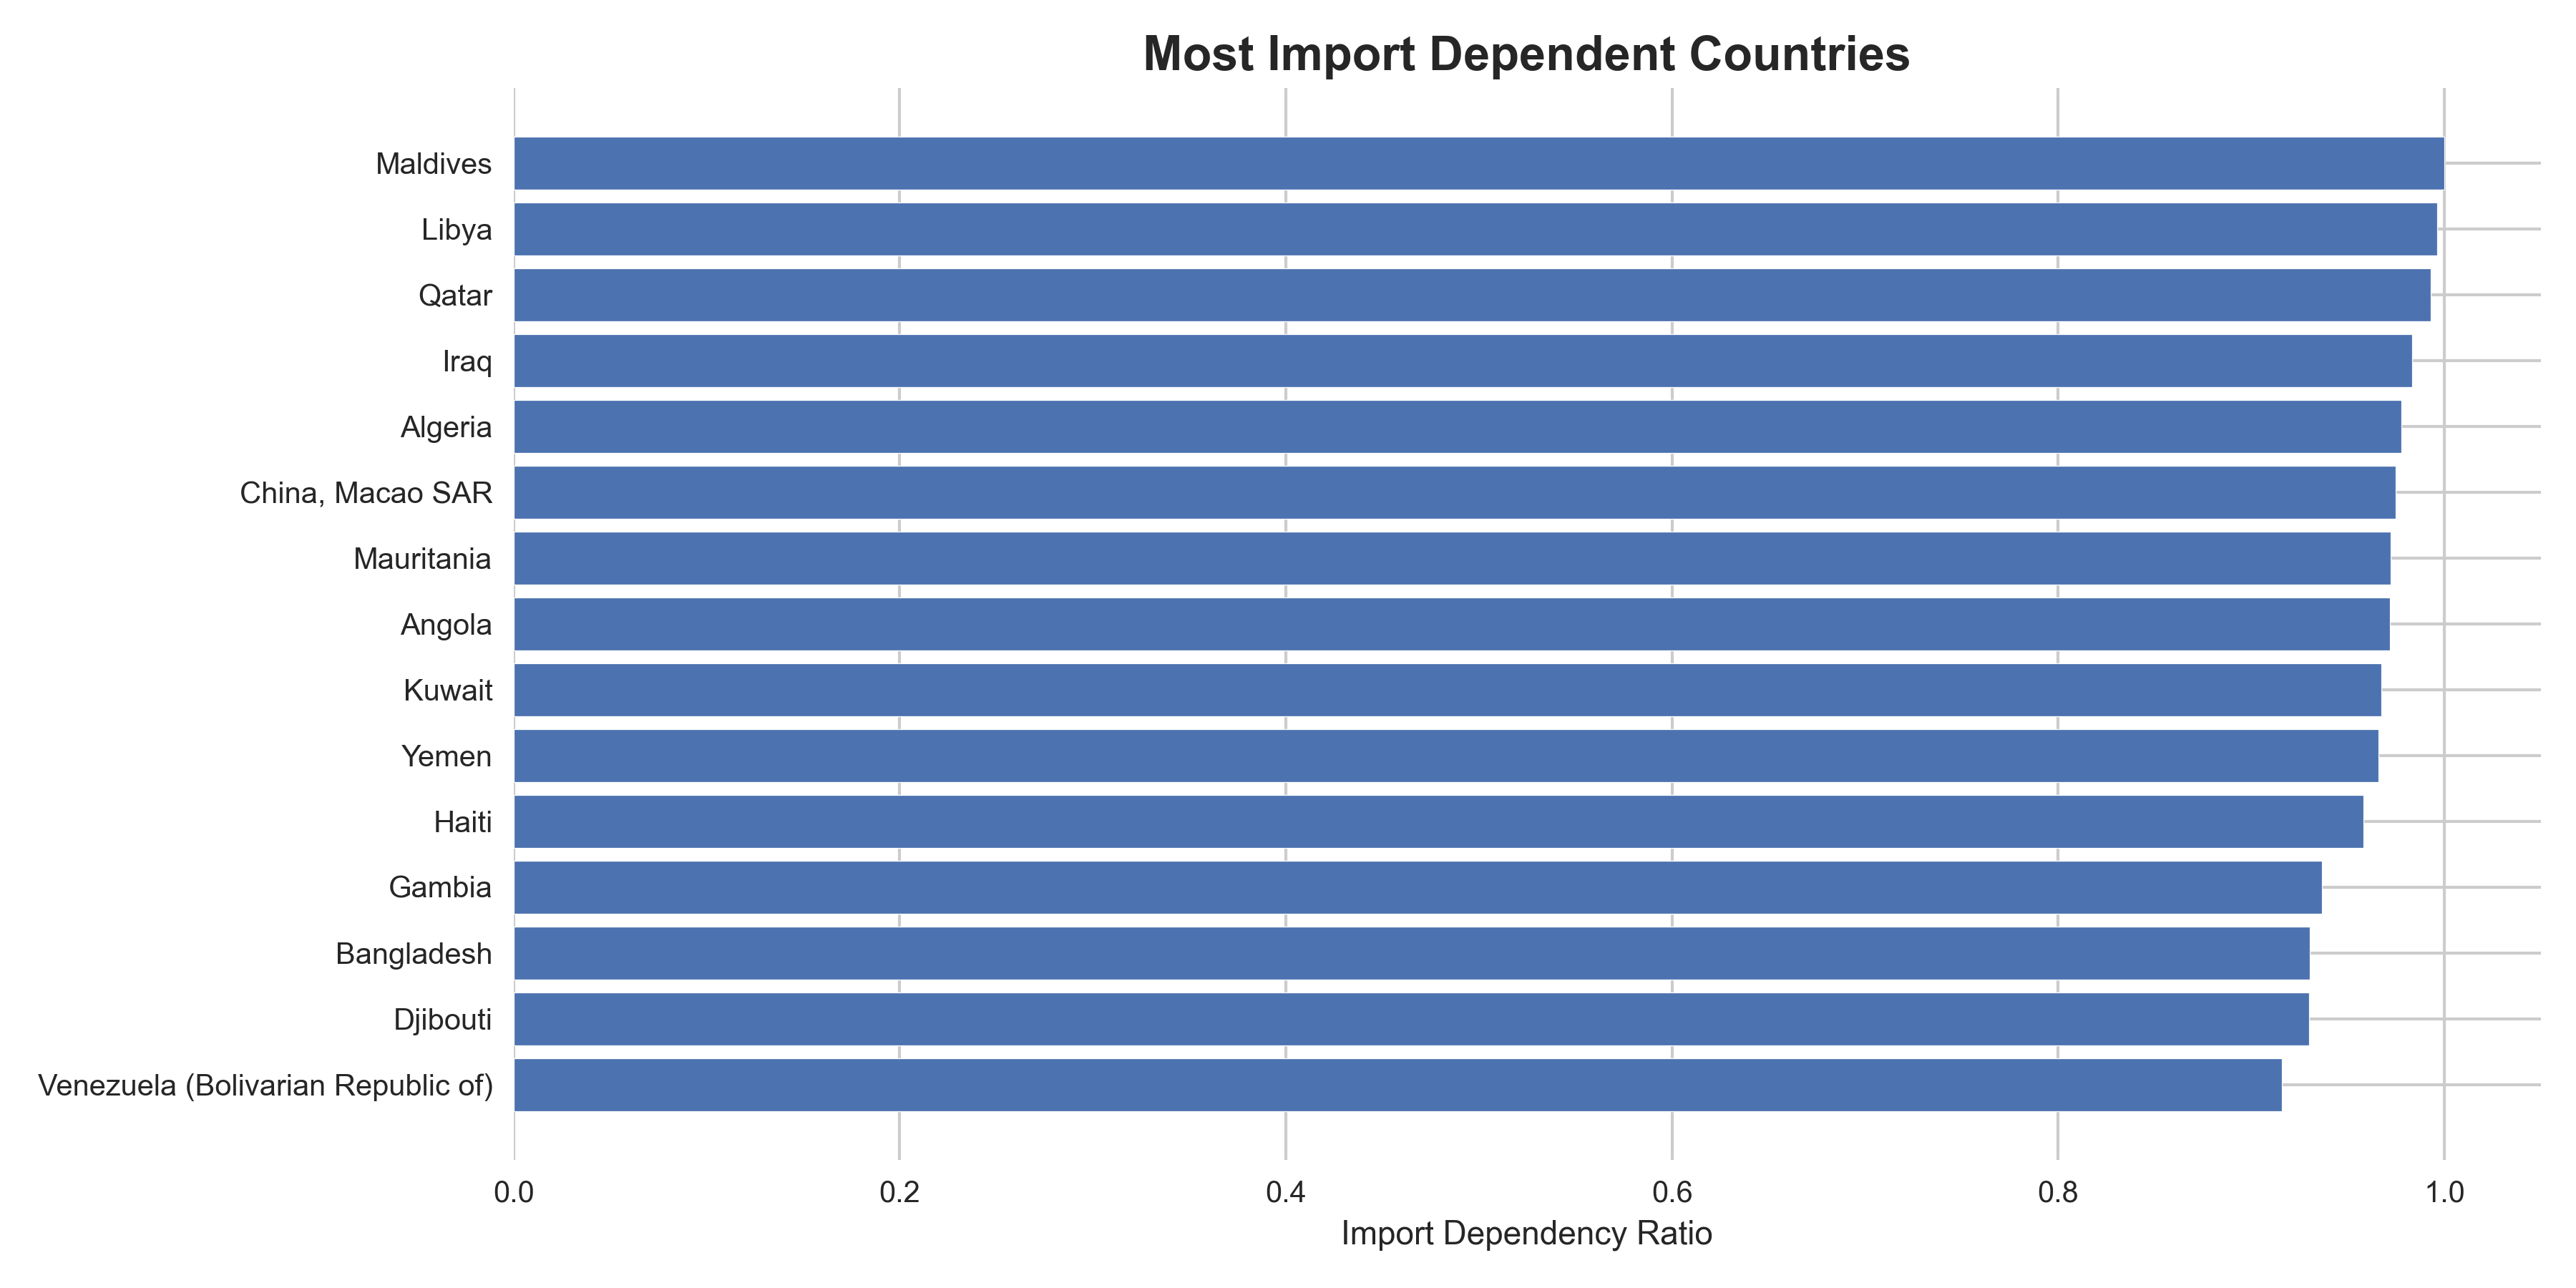
\includegraphics[width=\linewidth]{15_import_dependency.png}
    \caption{Import dependency (exposure to supplier failures).}
  \end{subfigure}
  \hfill
  \begin{subfigure}[t]{0.49\linewidth}
    \centering
    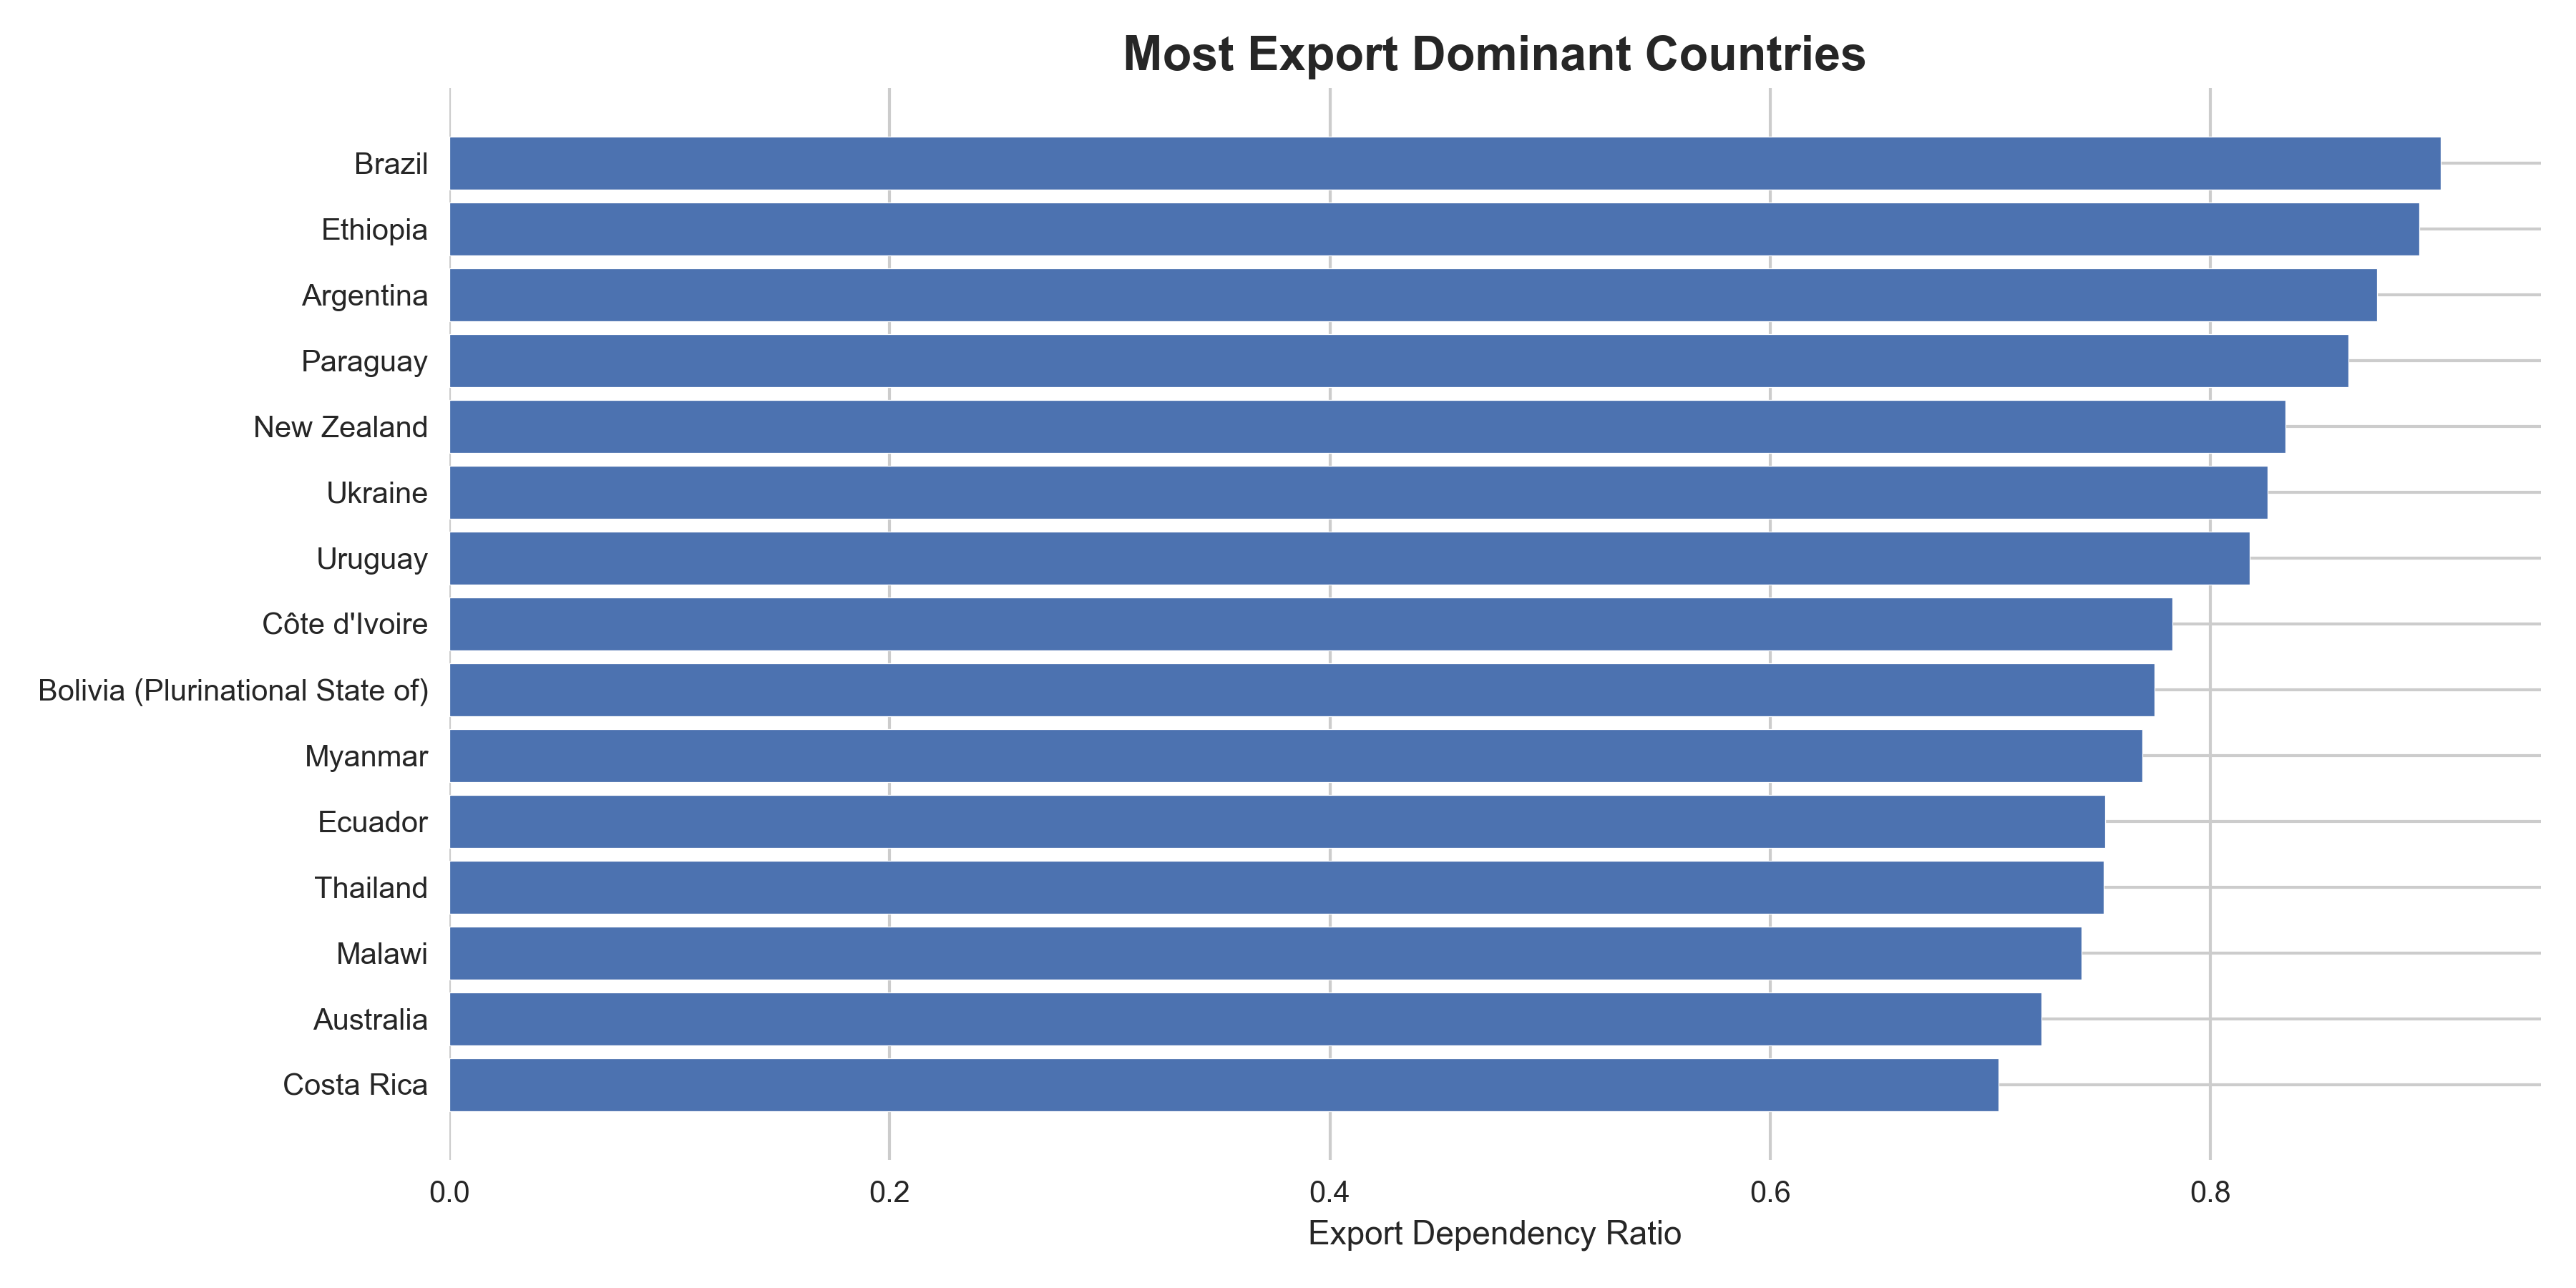
\includegraphics[width=\linewidth]{16_export_dependency.png}
    \caption{Export dependency (exposure to demand/corridor shocks).}
  \end{subfigure}
  \caption{Country dependency profiles highlight vulnerability to disruptions.}
  \label{fig:dependencies}
\end{figure}

\begin{figure}[H]
  \centering
  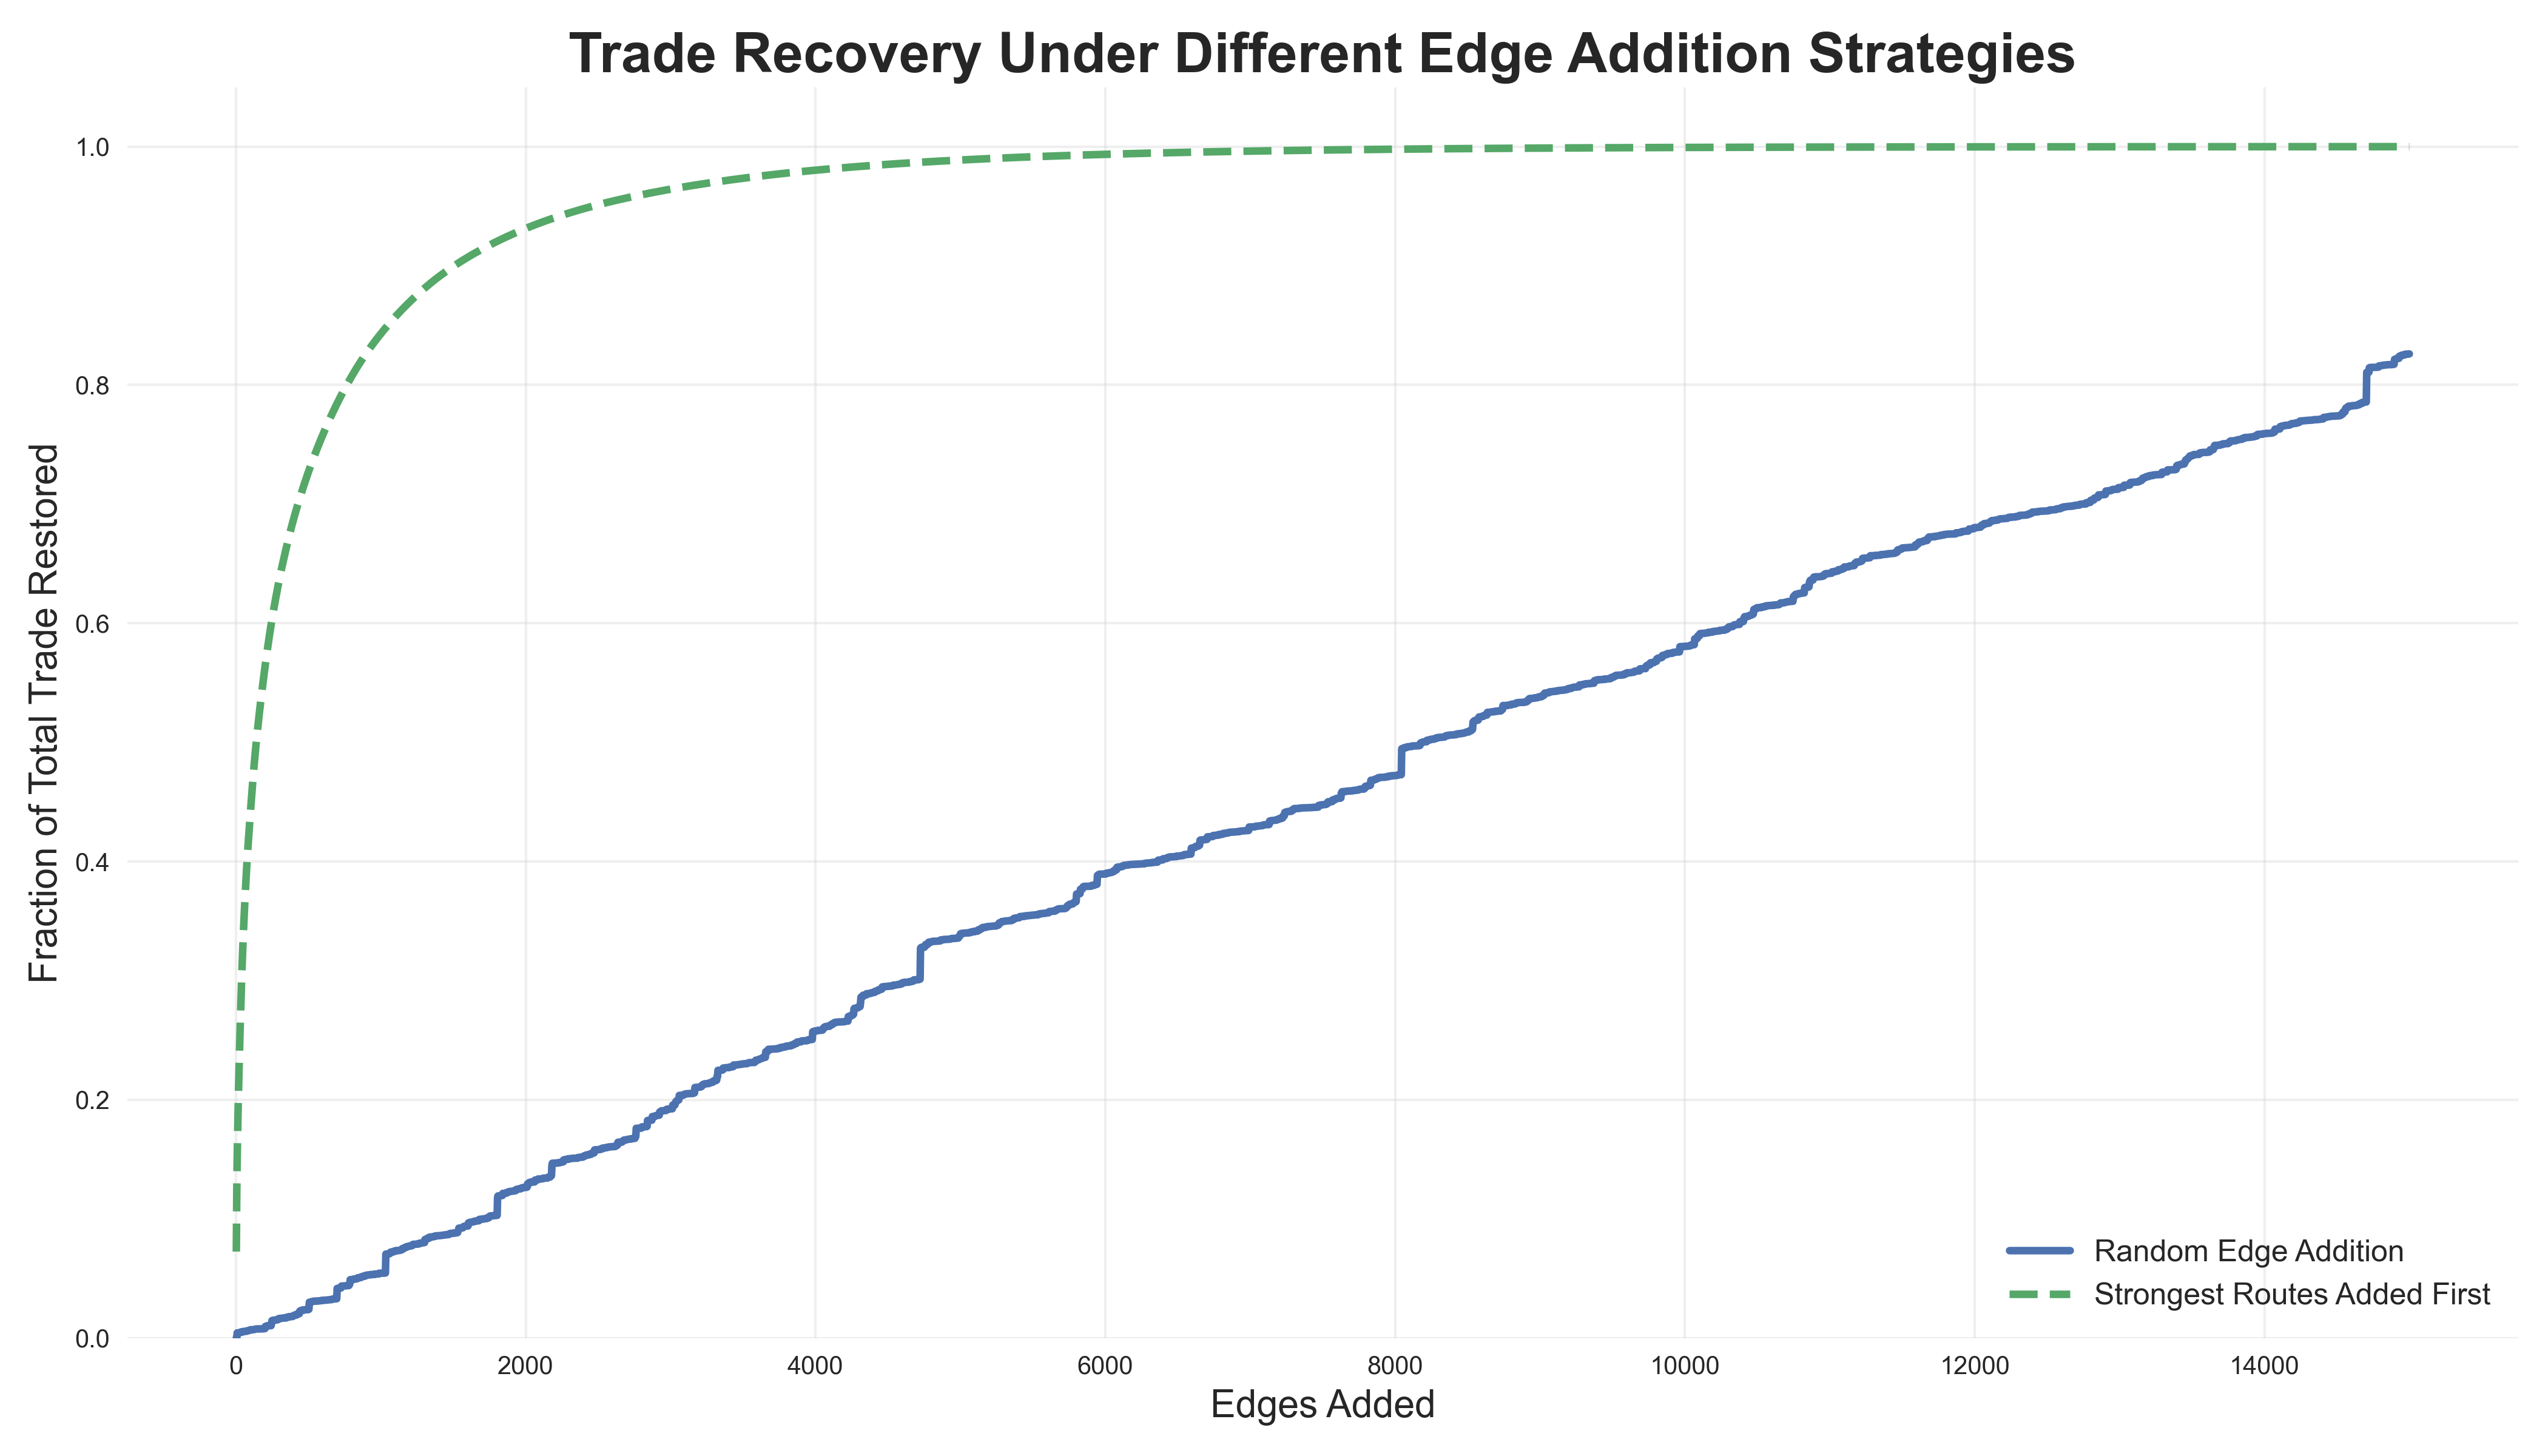
\includegraphics[width=0.98\linewidth]{42_edge_addition_trade_only.png}
  \caption{Mitigation via edge addition: restoring strongest corridors first recovers trade volume faster than random restoration.}
  \label{fig:edge-addition}
\end{figure}

\subsection{Network resilience summary table}
\begin{table}[H]
\centering
\begin{tabularx}{0.98\linewidth}{@{}l r X@{}}
\toprule
\textbf{Metric} & \textbf{Value} & \textbf{Interpretation} \\
\midrule
Nodes & 198 & Countries in the network \\
Edges & 18{,}242 & Directed routes (exporter $\rightarrow$ importer) \\
Density & 0.4677 & Closeness to a fully connected directed graph \\
Reciprocity & 0.7824 & Fraction of mutual links in both directions \\
Communities & 2 & Coarse blocs detected by topology-based modularity \\
Largest SCC & 198 & All countries mutually reachable (strong connectivity) \\
Assortativity & -0.3591 & Disassortative: hubs connect to low-degree countries \\
\bottomrule
\end{tabularx}
\caption{Resilience-related network metrics (values as reported in the dashboard summary).}
\label{tab:resilience-summary}
\end{table}

\paragraph{Fragility findings.}
\begin{itemize}
  \item Robust to random shocks but fragile to targeted disruption.
  \item Removing a small set of critical nodes/corridors can eliminate most trade value quickly.
  \item Practical resilience: diversify suppliers and add redundancy for high-impact corridors.
\end{itemize}

\section{Final Findings \& Network Classification}
\subsection{Network type: heavy-tail with strong concentration}
\begin{figure}[H]
  \centering
  \begin{subfigure}[t]{0.49\linewidth}
    \centering
    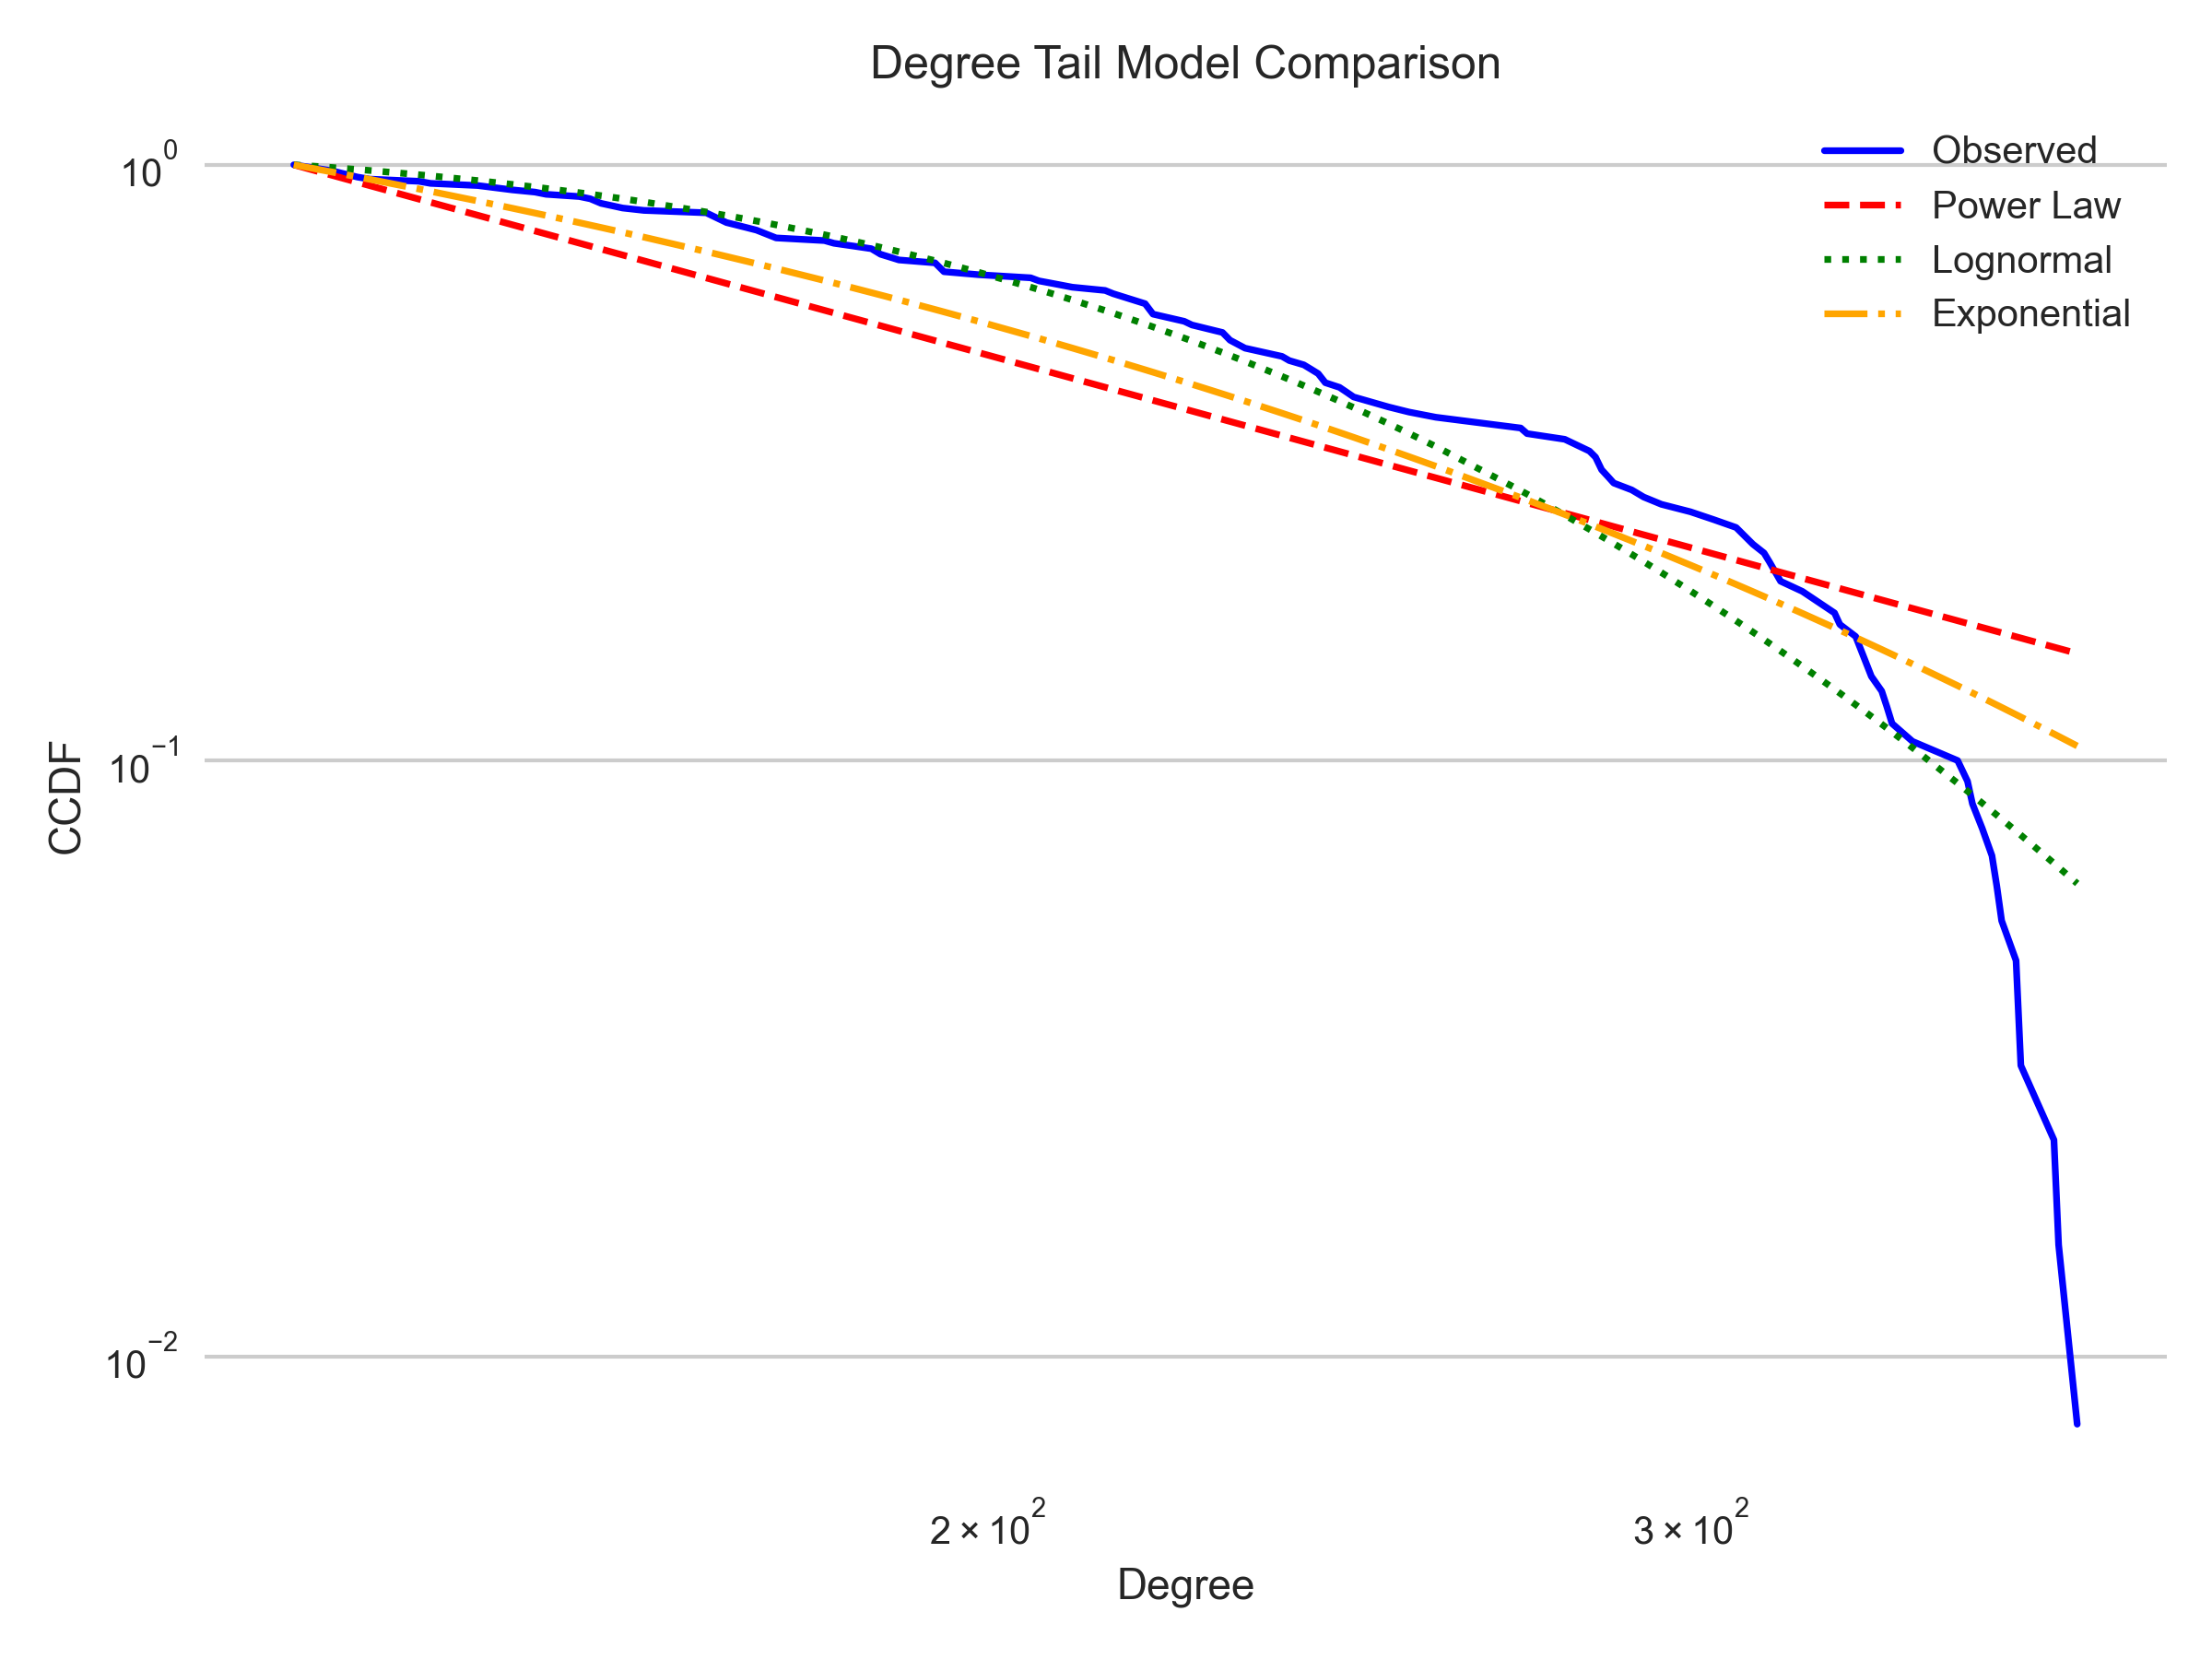
\includegraphics[width=\linewidth]{28_model_ccdf_compare.png}
    \caption{Degree tail model comparison (CCDF).}
  \end{subfigure}
  \hfill
  \begin{subfigure}[t]{0.49\linewidth}
    \centering
    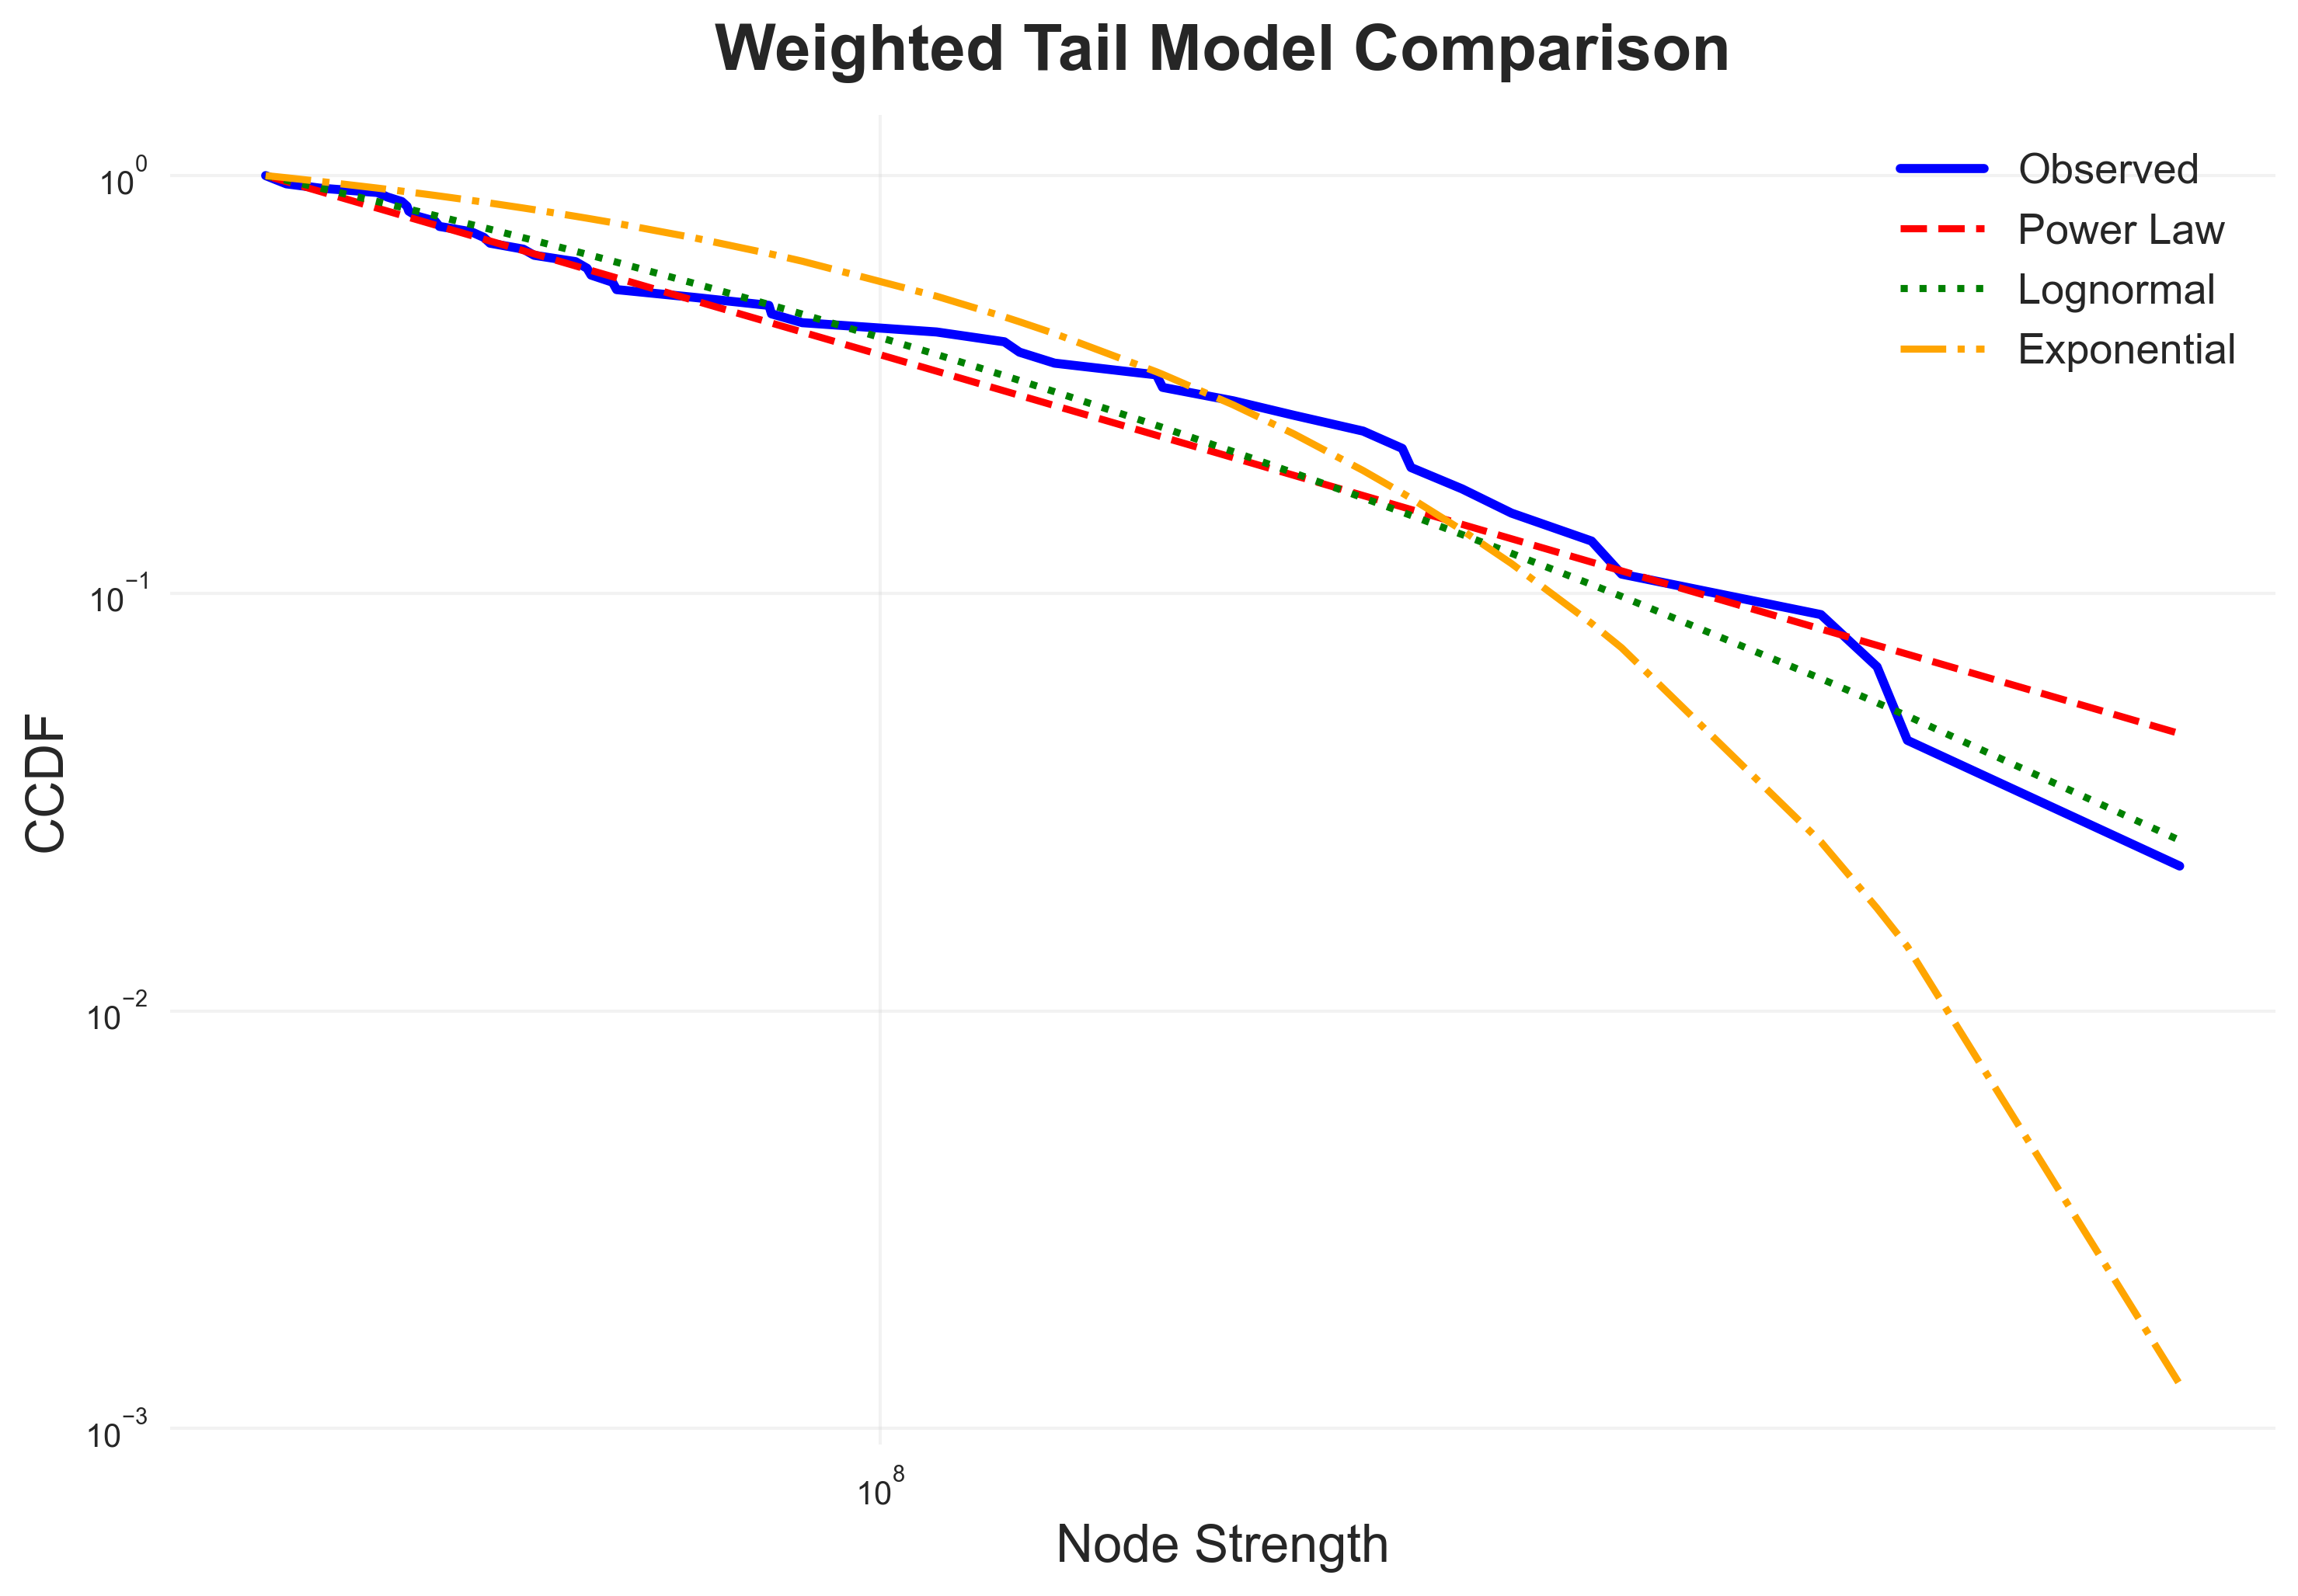
\includegraphics[width=\linewidth]{weighted_tail_model_comparison.png}
    \caption{Weighted strength tail model comparison.}
  \end{subfigure}
  \caption{Model comparisons suggest heavy tails (often lognormal-favored vs pure power law for degree).}
  \label{fig:model-comparisons}
\end{figure}

\begin{figure}[H]
  \centering
  \begin{subfigure}[t]{0.49\linewidth}
    \centering
    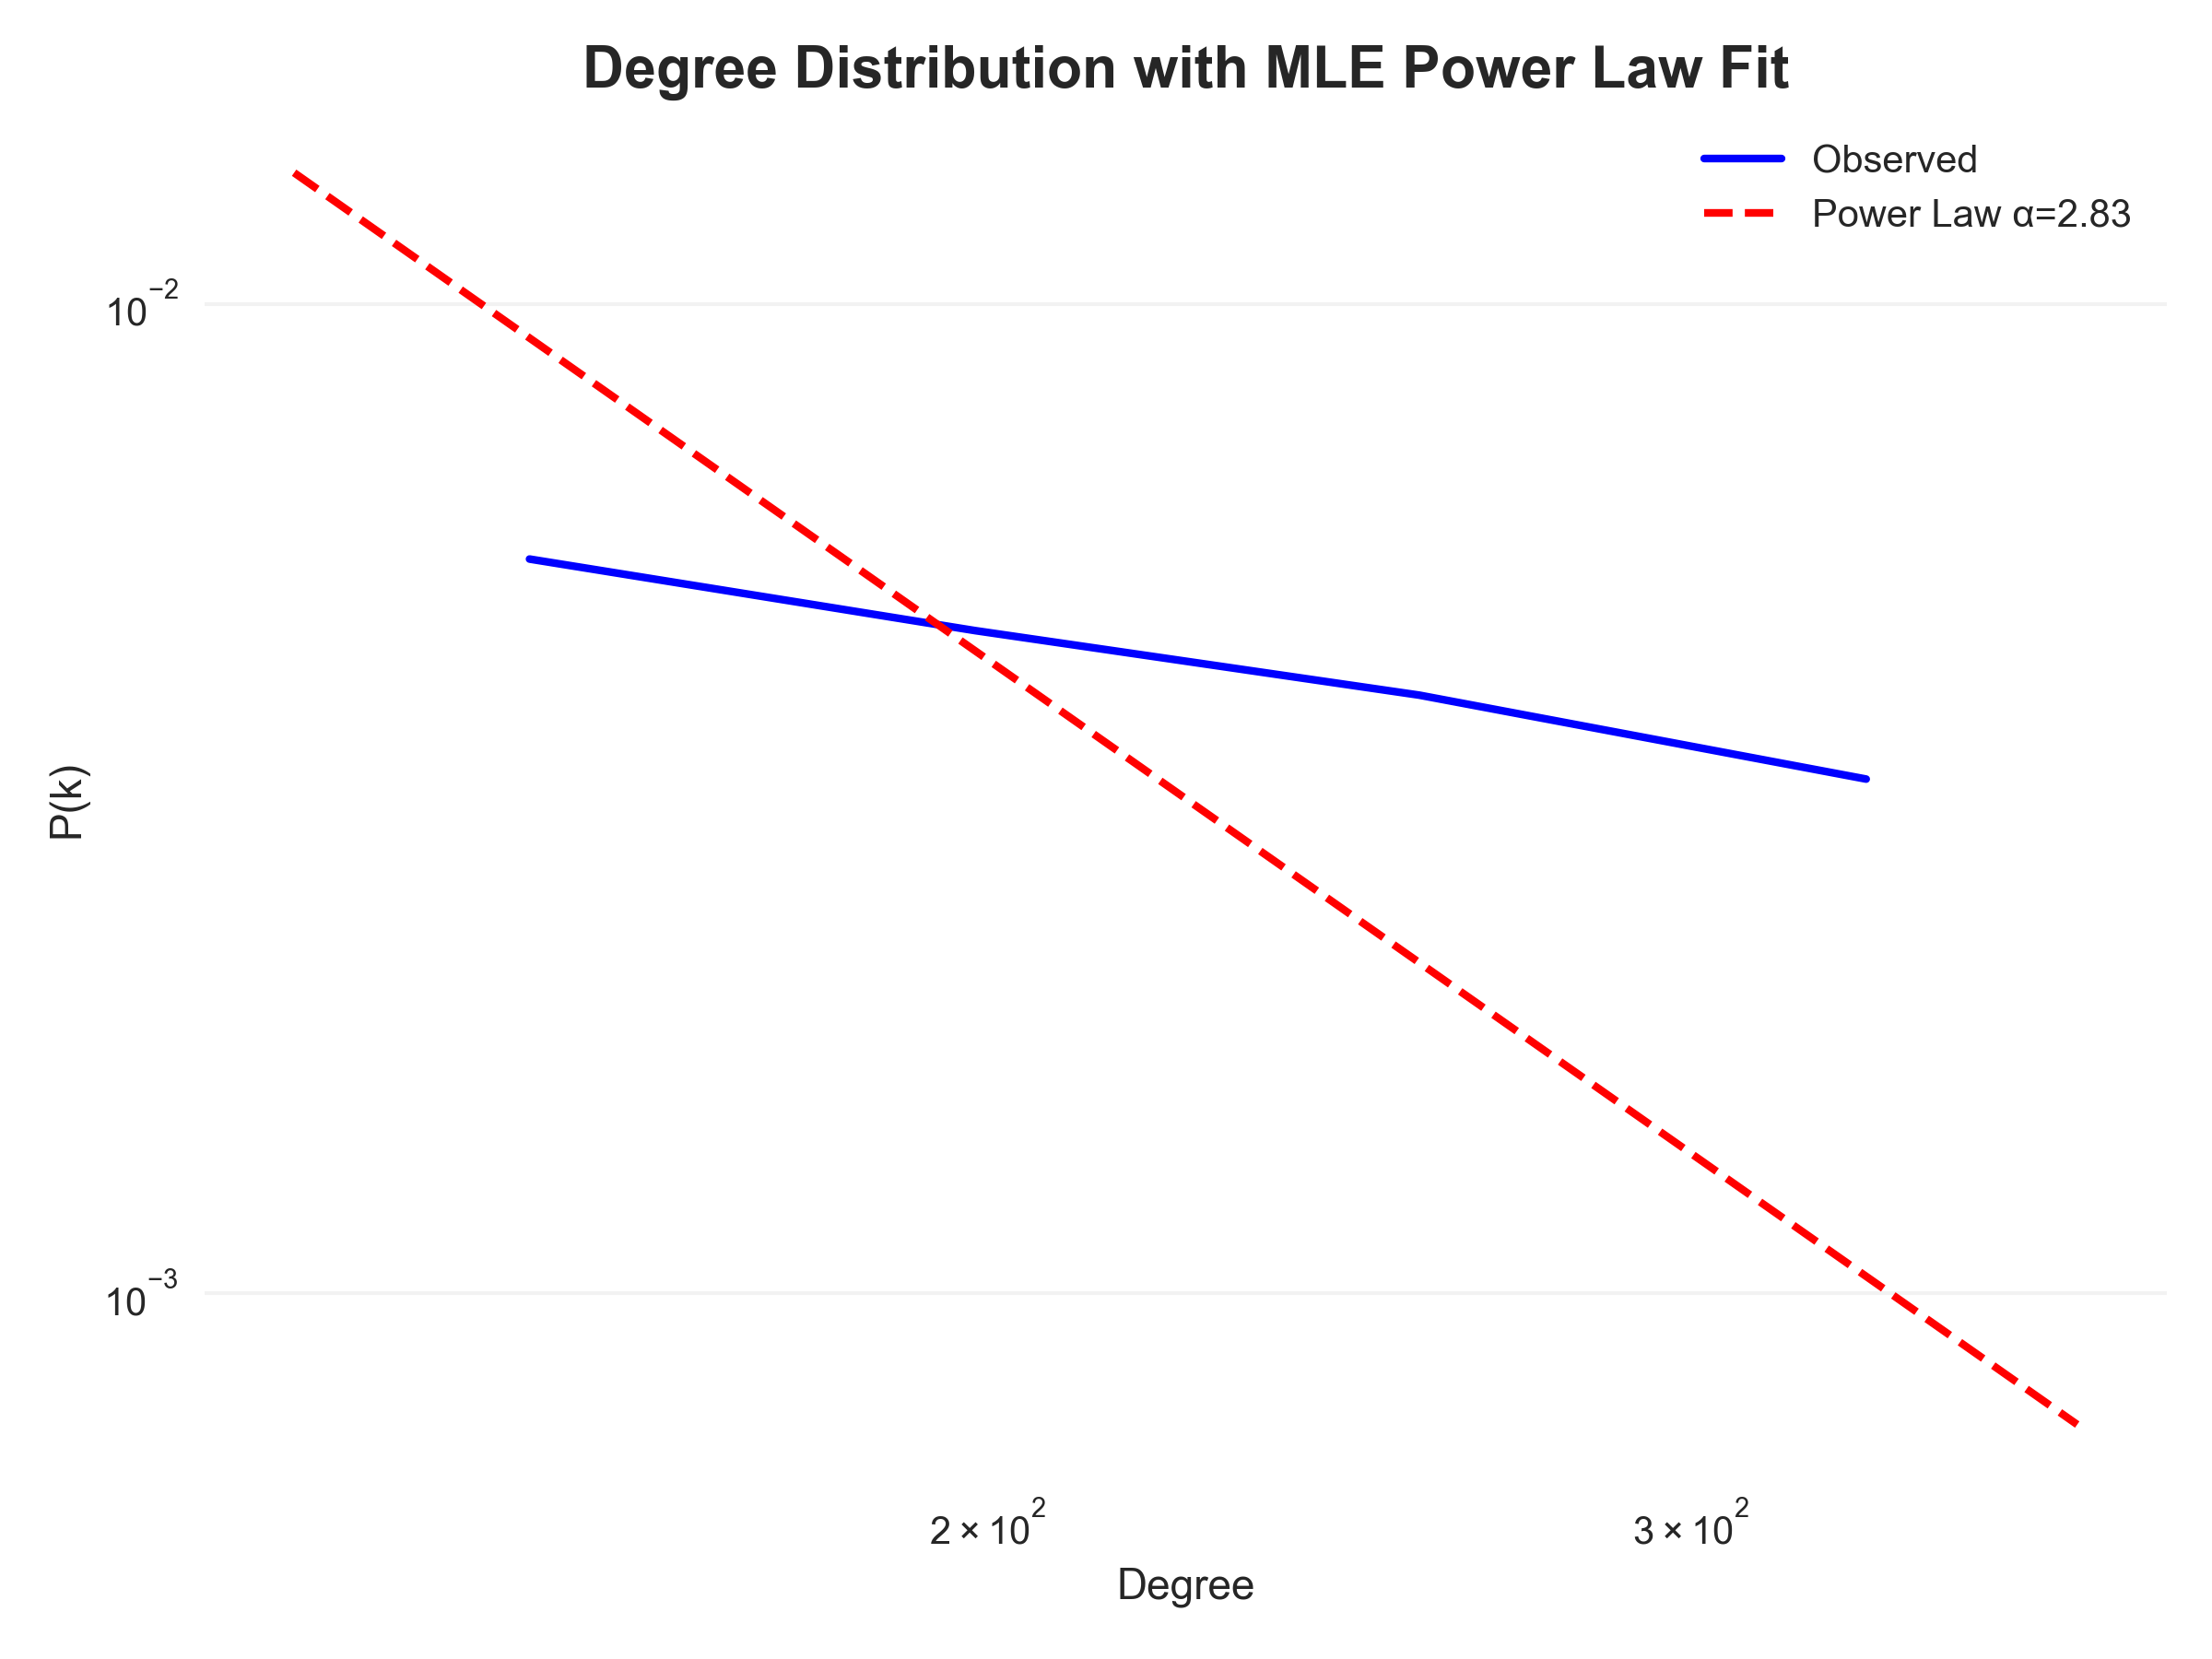
\includegraphics[width=\linewidth]{powerlaw_fit_degree.png}
    \caption{Degree tail fit (reported $\alpha=2.831$, $x_{\min}=134$).}
  \end{subfigure}
  \hfill
  \begin{subfigure}[t]{0.49\linewidth}
    \centering
    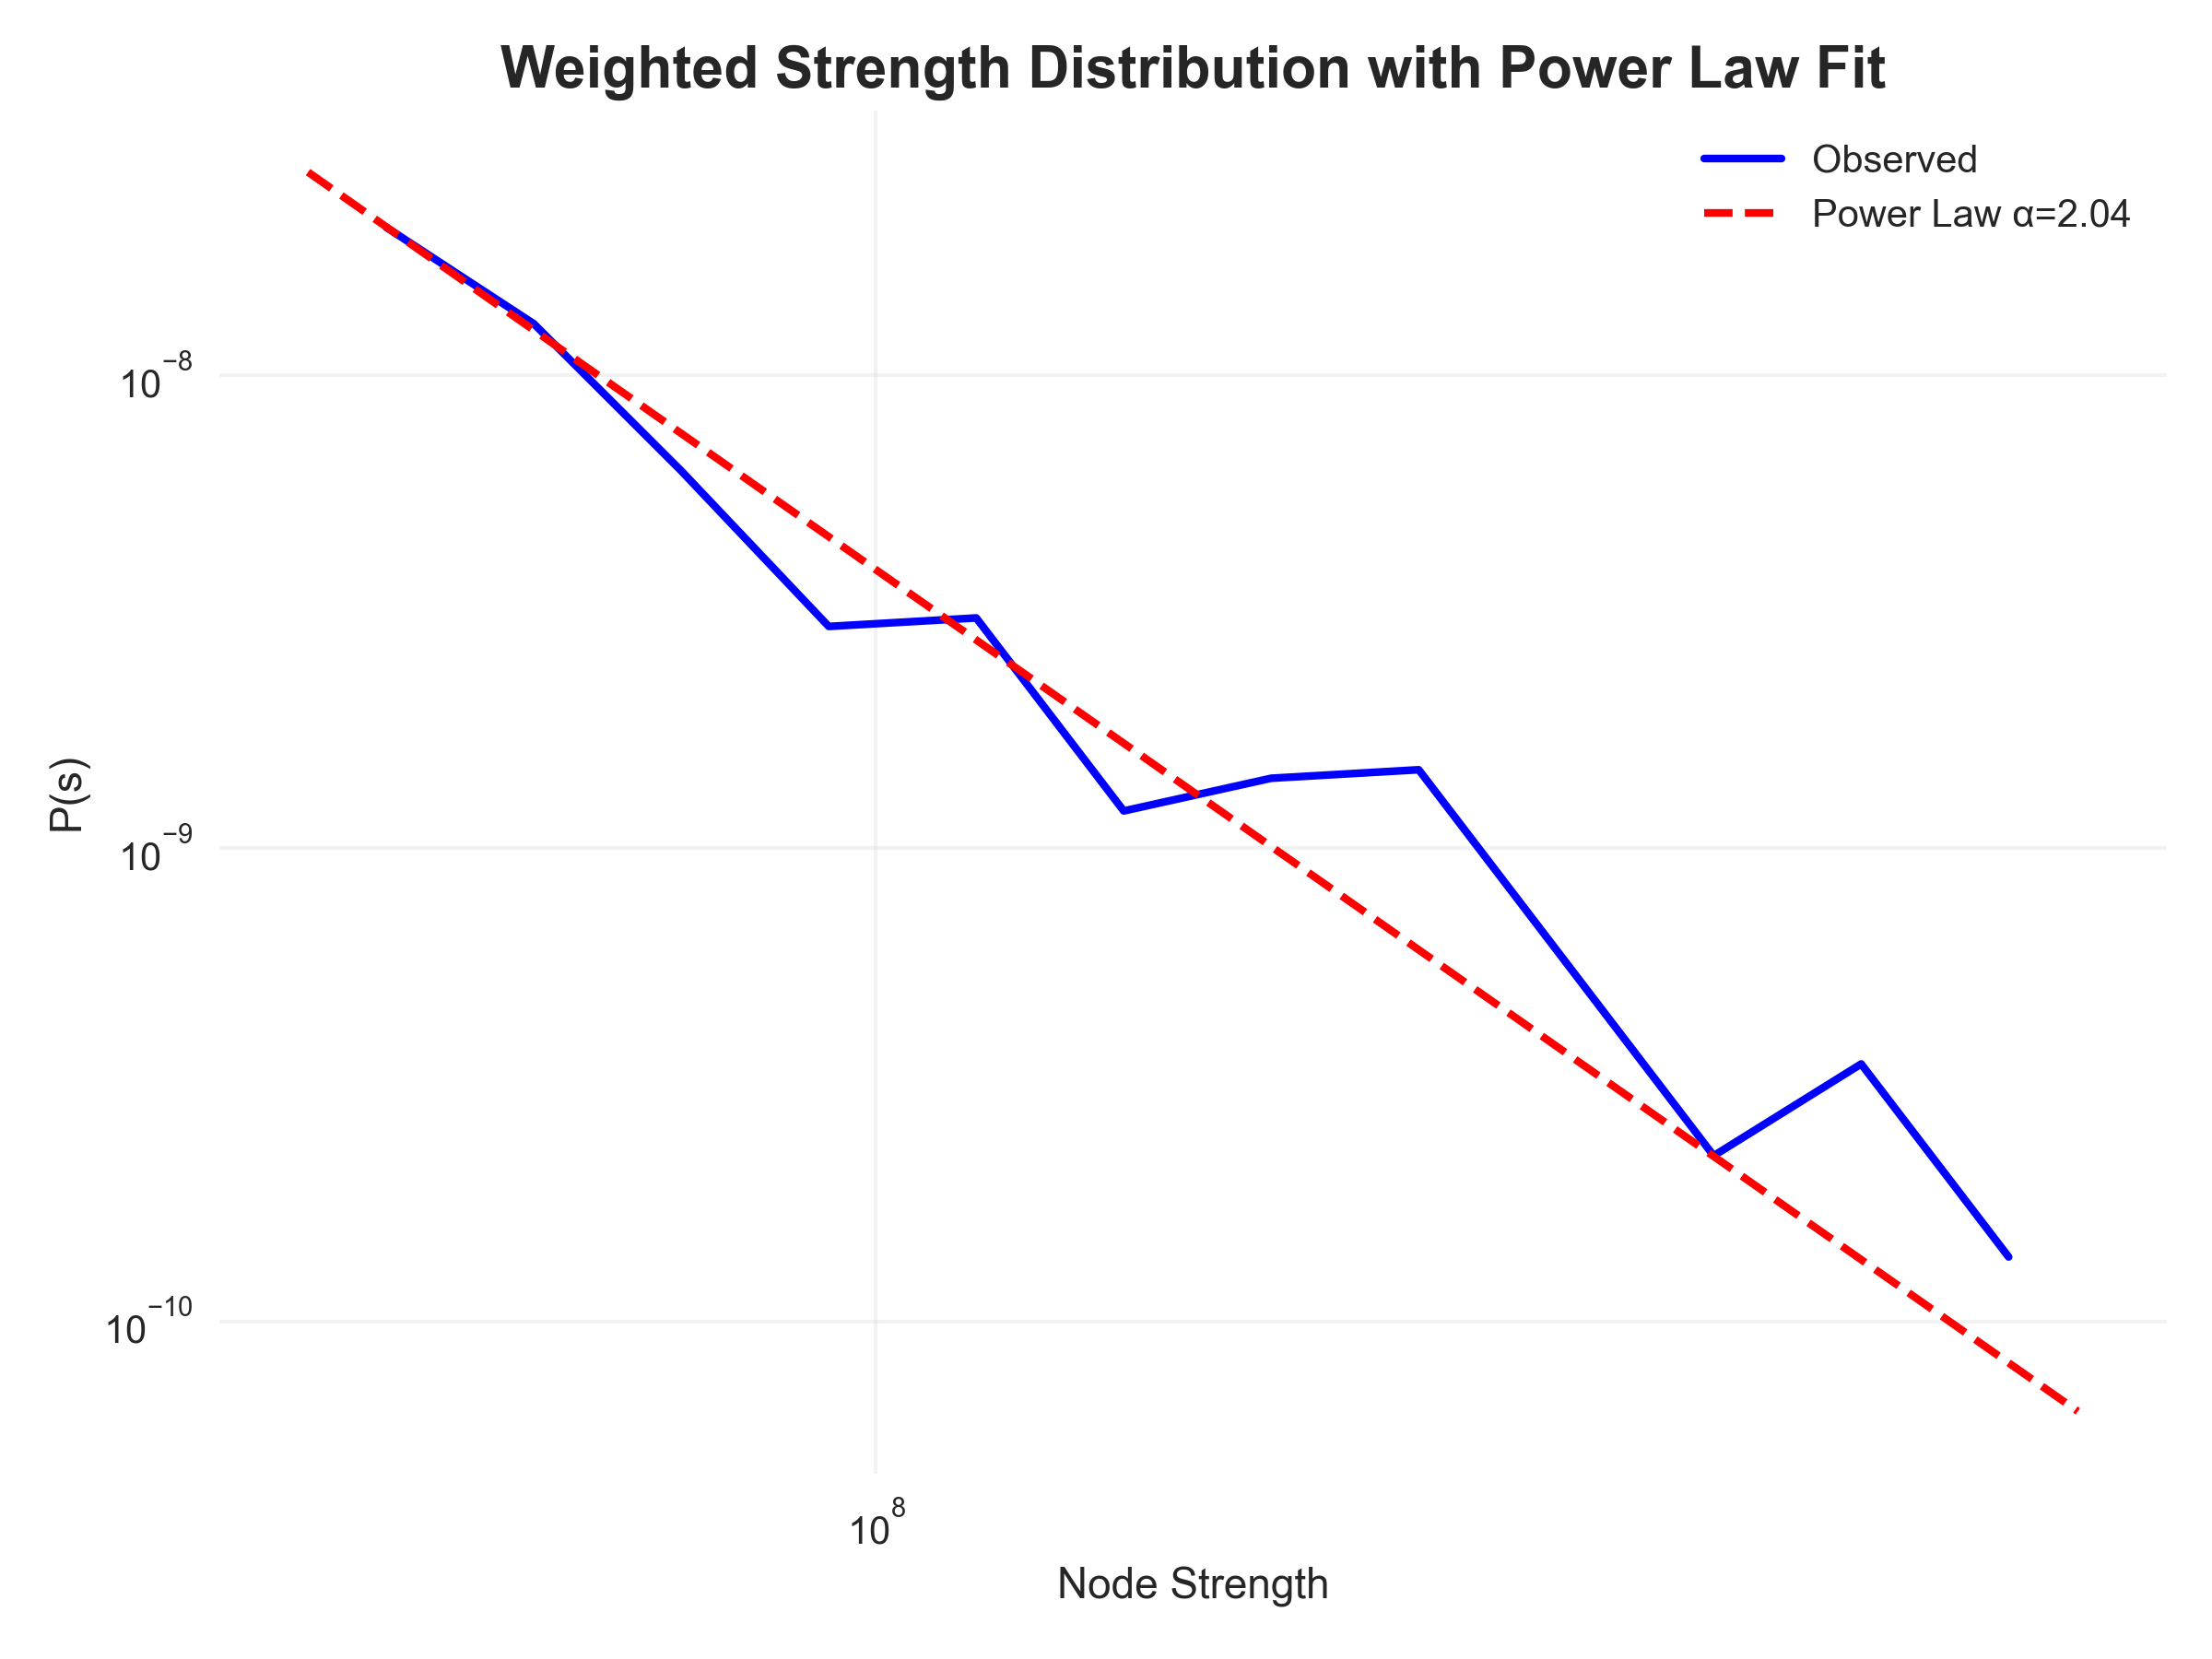
\includegraphics[width=\linewidth]{powerlaw_fit_weighted_strength.png}
    \caption{Strength tail fit (reported $\alpha=2.041$, $x_{\min}\approx 38.7\text{M}$).}
  \end{subfigure}
  \caption{Tail fits for degree and weighted strength (as reported in the dashboard).}
  \label{fig:tail-fits}
\end{figure}

\subsection{Concentration recap (rank plots)}
\begin{figure}[H]
  \centering
  \begin{subfigure}[t]{0.49\linewidth}
    \centering
    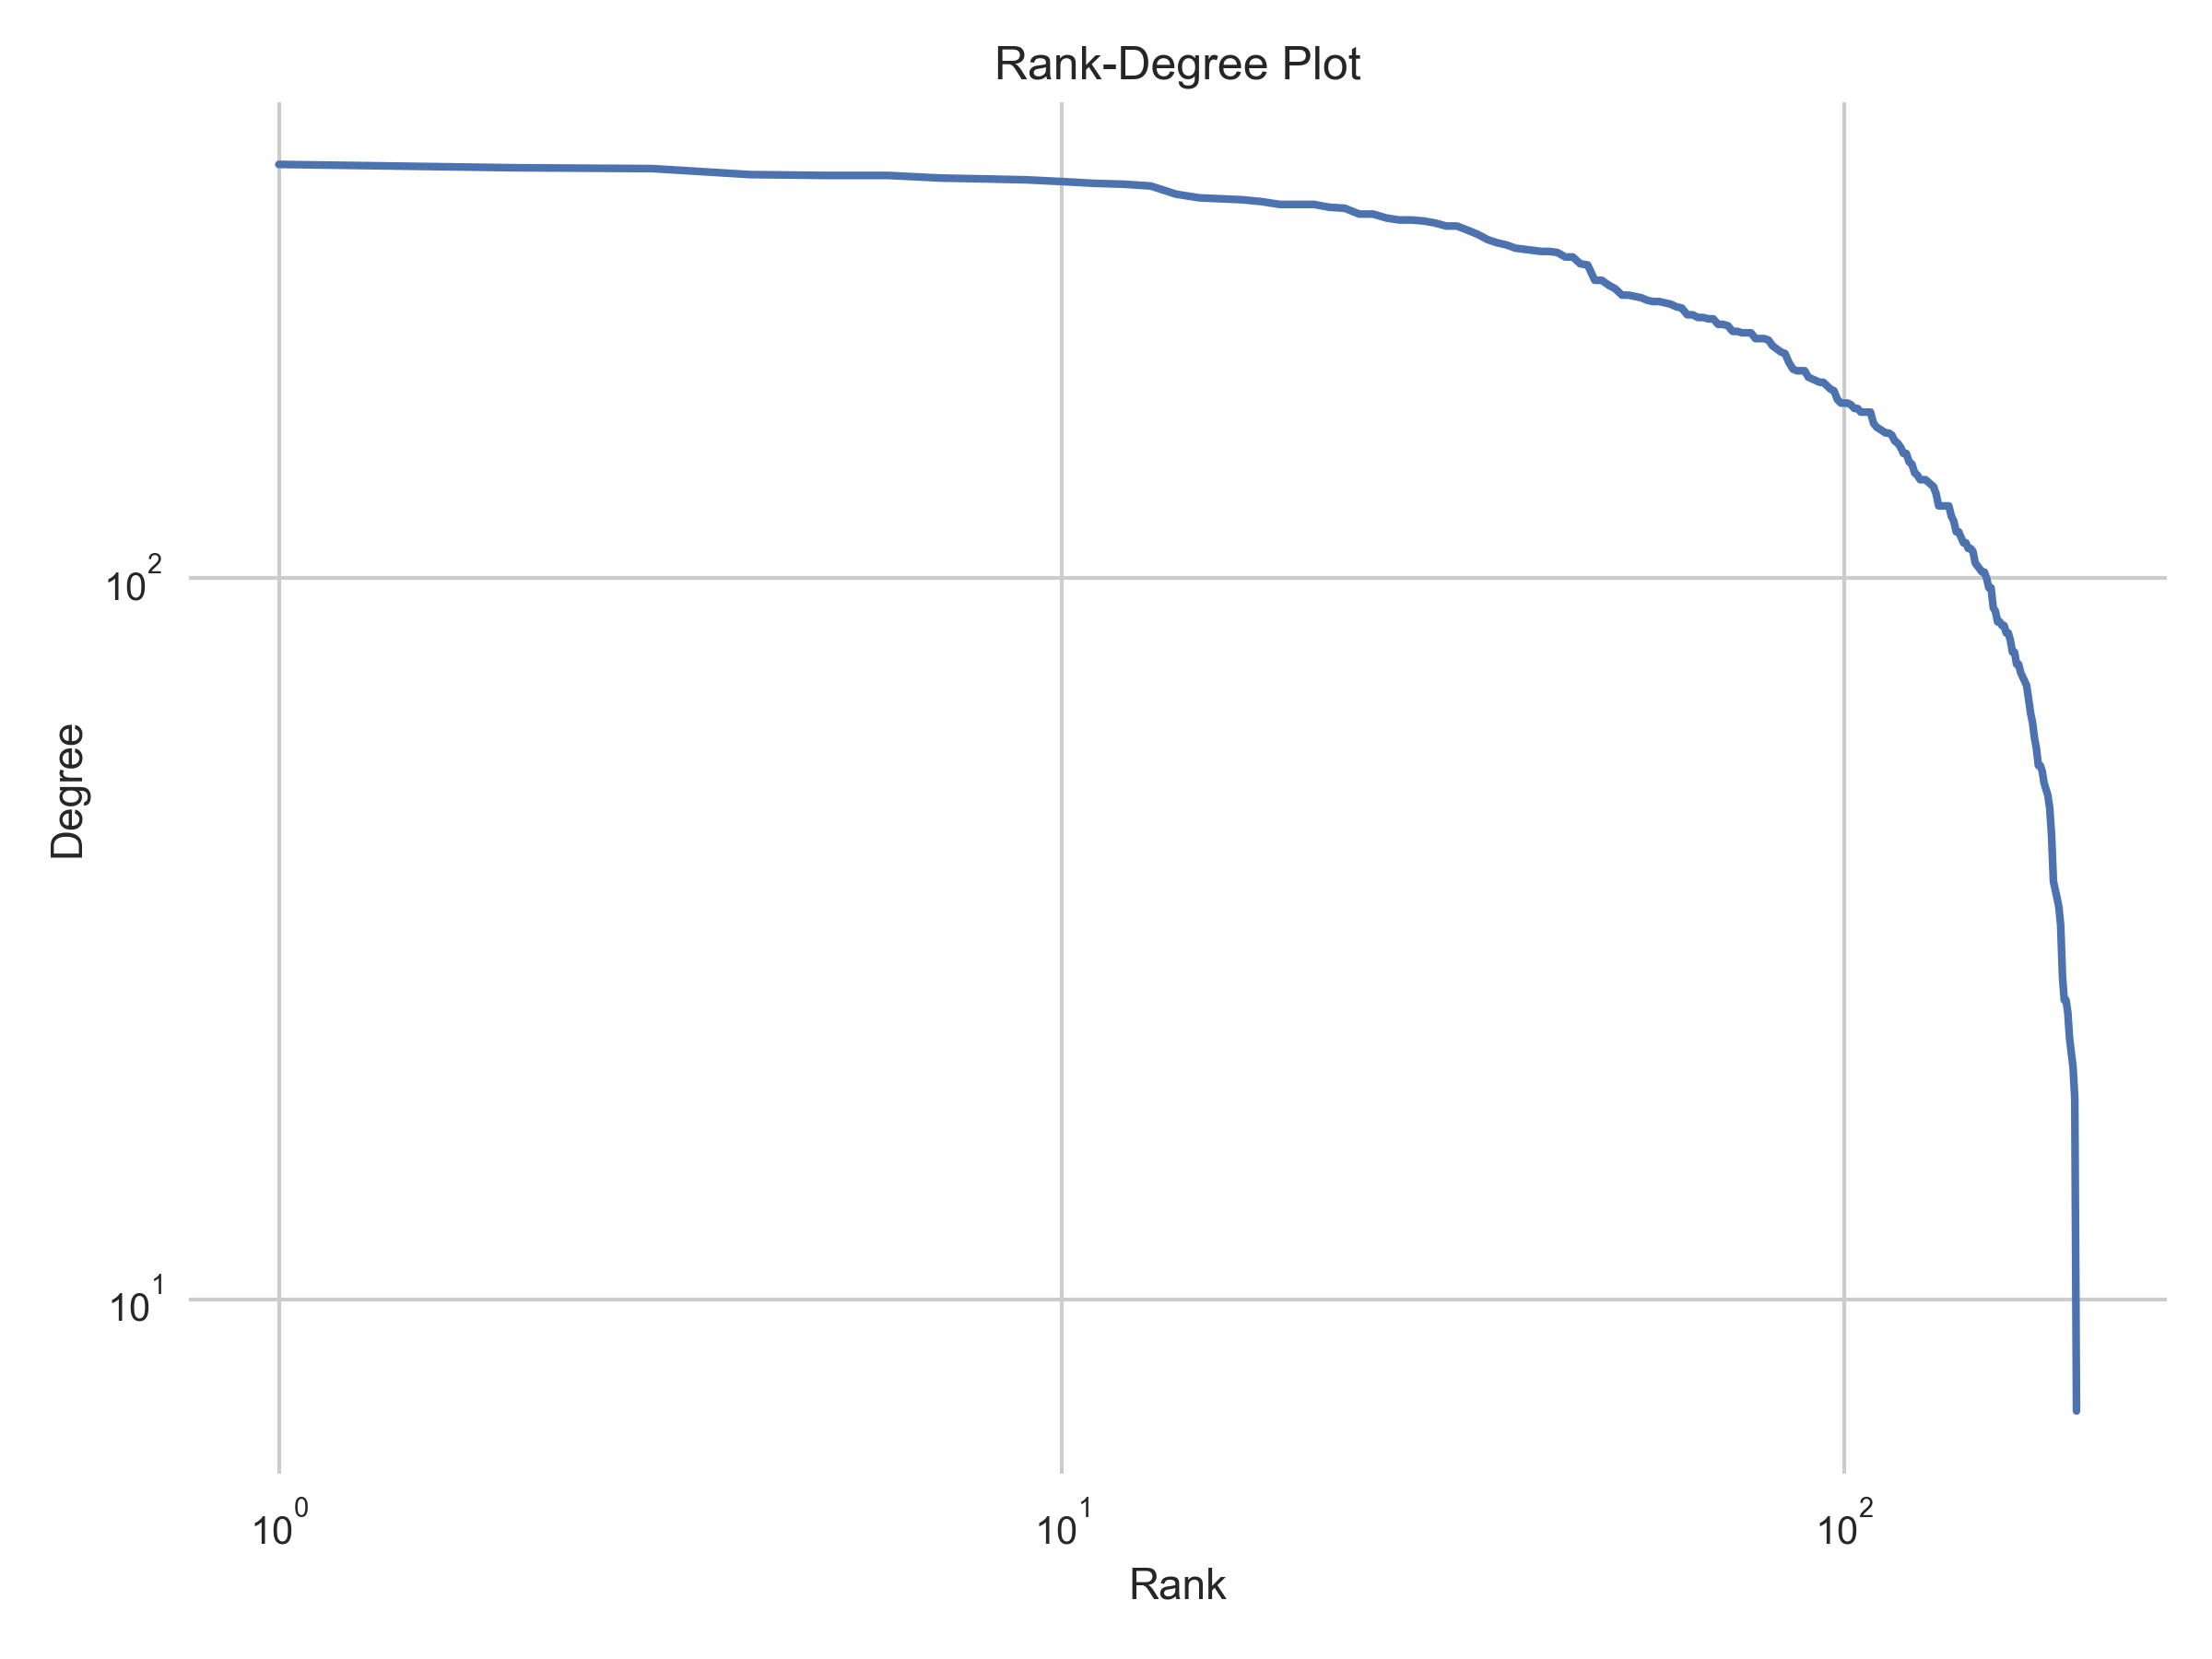
\includegraphics[width=\linewidth]{29_rank_degree_plot.png}
    \caption{Rank vs degree (connectivity concentration).}
  \end{subfigure}
  \hfill
  \begin{subfigure}[t]{0.49\linewidth}
    \centering
    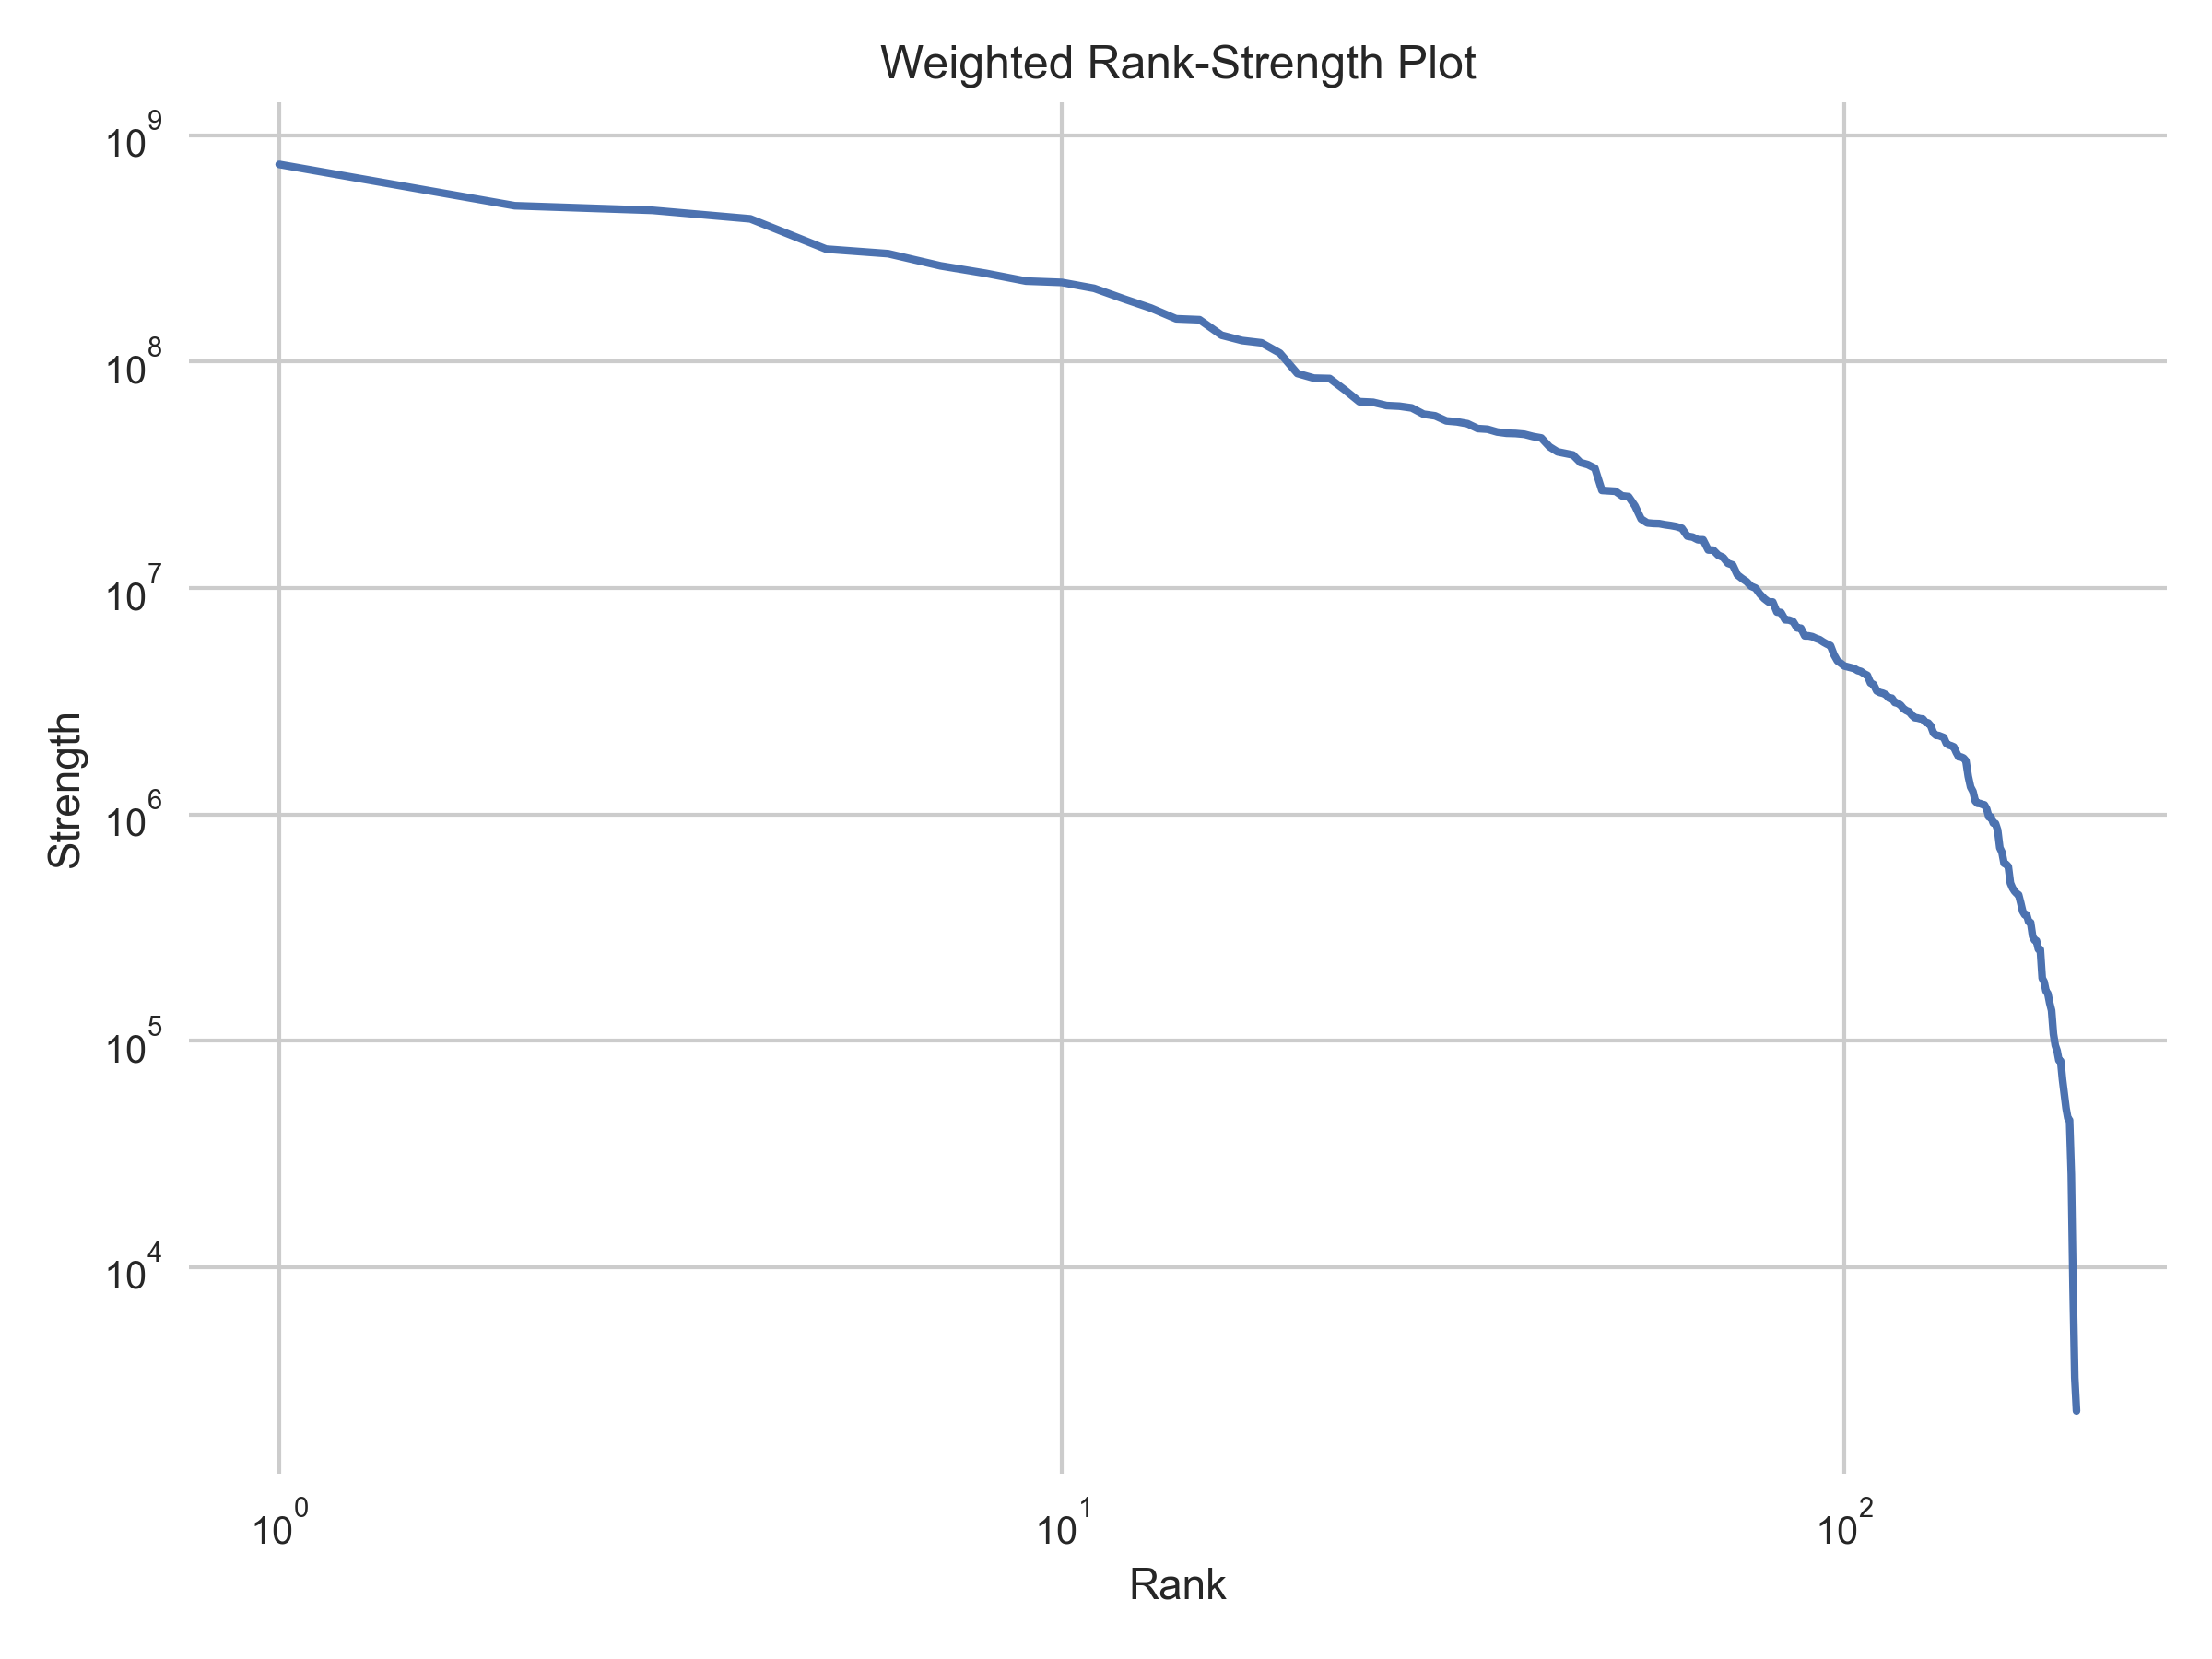
\includegraphics[width=\linewidth]{weighted_strength_rank_plot.png}
    \caption{Rank vs strength (value concentration).}
  \end{subfigure}
  \caption{Few countries dominate connectivity; even fewer dominate trade value.}
  \label{fig:rank-plots}
\end{figure}

\subsection{Quantitative summary table}
\begin{table}[H]
\centering
\begin{tabularx}{0.98\linewidth}{@{}l X@{}}
\toprule
\textbf{Characteristic} & \textbf{Measurement (reported)} \\
\midrule
Degree tail & $\alpha=2.831$, $K_{\min}=134$; PL vs lognormal: $R=-30.745$ \\
Strength tail & $\alpha=2.041$, $K_{\min}\approx 38.7\text{M}$; PL vs lognormal: $R=-0.878$ \\
Total flow & Total trade weight sum $\approx 3{,}734{,}925{,}964$ \\
\bottomrule
\end{tabularx}
\caption{Tail and flow summary metrics (as reported in the dashboard).}
\label{tab:quant-summary}
\end{table}

\subsection{Key findings}
\begin{itemize}
  \item Global food trade is concentrated around a few hub countries.
  \item Some countries act as bridges connecting separate trade blocs.
  \item Structural importance differs from raw trade volume.
  \item A few routes function as critical global trade corridors.
  \item The network survives random shocks better than targeted attacks.
\end{itemize}

\end{document}
